% A LaTeX template for MSc Thesis submissions to
% Politecnico di Milano (PoliMi) - School of Industrial and Information Engineering
%
% S. Bonetti, A. Gruttadauria, G. Mescolini, A. Zingaro
% e-mail: template-tesi-ingind@polimi.it
%
% Last Revision: October 2021
%
% Copyright 2021 Politecnico di Milano, Italy. NC-BY

\documentclass{Configuration_Files/PoliMi3i_thesis}

%------------------------------------------------------------------------------
%	REQUIRED PACKAGES AND  CONFIGURATIONS
%------------------------------------------------------------------------------

% CONFIGURATIONS
\usepackage{parskip} % For paragraph layout
\usepackage{setspace} % For using single or double spacing
\usepackage{emptypage} % To insert empty pages
\usepackage{multicol} % To write in multiple columns (executive summary)
\setlength\columnsep{15pt} % Column separation in executive summary
\setlength\parindent{0pt} % Indentation
\raggedbottom

% PACKAGES FOR TITLES
\usepackage{titlesec}
% \titlespacing{\section}{left spacing}{before spacing}{after spacing}
\titlespacing{\section}{0pt}{3.3ex}{2ex}
\titlespacing{\subsection}{0pt}{3.3ex}{1.65ex}
\titlespacing{\subsubsection}{0pt}{3.3ex}{1ex}
\usepackage{color}

% PACKAGES FOR LANGUAGE AND FONT
\usepackage[english]{babel} % The document is in English
\usepackage[utf8]{inputenc} % UTF8 encoding
\usepackage[T1]{fontenc} % Font encoding
\usepackage[11pt]{moresize} % Big fonts

% PACKAGES FOR IMAGES
\usepackage{graphicx}
\usepackage{transparent} % Enables transparent images
\usepackage{eso-pic} % For the background picture on the title page
\usepackage{subfig} % Numbered and caption subfigures using \subfloat.
\usepackage{tikz} % A package for high-quality hand-made figures.
\usetikzlibrary{}
\graphicspath{{./Images/}} % Directory of the images
\usepackage{caption} % Coloured captions
\usepackage{xcolor} % Coloured captions
\usepackage{amsthm,thmtools,xcolor} % Coloured "Theorem"
\usepackage{float}

% STANDARD MATH PACKAGES
\usepackage{amsmath}
\usepackage{amsthm}
\usepackage{amssymb}
\usepackage{amsfonts}
\usepackage{bm}
\usepackage[overload]{empheq} % For braced-style systems of equations.
\usepackage{fix-cm} % To override original LaTeX restrictions on sizes

% PACKAGES FOR TABLES
\usepackage{tabularx}
\usepackage{longtable} % Tables that can span several pages
\usepackage{colortbl}

% PACKAGES FOR ALGORITHMS (PSEUDO-CODE)
\usepackage{algorithm}
\usepackage{algorithmic}


% PACKAGES FOR REFERENCES & BIBLIOGRAPHY
\usepackage[colorlinks=true,linkcolor=black,anchorcolor=black,citecolor=black,filecolor=black,menucolor=black,runcolor=black,urlcolor=black]{hyperref} % Adds clickable links at references
\usepackage{cleveref}
\usepackage[square, numbers, sort&compress]{natbib} % Square brackets, citing references with numbers, citations sorted by appearance in the text and compressed
\bibliographystyle{abbrvnat} % You may use a different style adapted to your field

% OTHER PACKAGES
\usepackage{pdfpages} % To include a pdf file
\usepackage{afterpage}
\usepackage{lipsum} % DUMMY PACKAGE
\usepackage{fancyhdr} % For the headers
\usepackage{listings}


% Input of configuration file. Do not change config.tex file unless you really know what you are doing.
% Define blue color typical of polimi
\definecolor{bluepoli}{cmyk}{0.4,0.1,0,0.4}

% Custom theorem environments
\declaretheoremstyle[
  headfont=\color{bluepoli}\normalfont\bfseries,
  bodyfont=\color{black}\normalfont\itshape,
]{colored}

% Set-up caption colors
\captionsetup[figure]{labelfont={color=bluepoli}} % Set colour of the captions
\captionsetup[table]{labelfont={color=bluepoli}} % Set colour of the captions
\captionsetup[algorithm]{labelfont={color=bluepoli}} % Set colour of the captions

\theoremstyle{colored}
\newtheorem{theorem}{Theorem}[chapter]
\newtheorem{proposition}{Proposition}[chapter]

% Enhances the features of the standard "table" and "tabular" environments.
\newcommand\T{\rule{0pt}{2.6ex}}
\newcommand\B{\rule[-1.2ex]{0pt}{0pt}}

% Pseudo-code algorithm descriptions.
\newcounter{algsubstate}
\renewcommand{\thealgsubstate}{\alph{algsubstate}}
\newenvironment{algsubstates}
  {\setcounter{algsubstate}{0}%
   \renewcommand{\STATE}{%
     \stepcounter{algsubstate}%
     \Statex {\small\thealgsubstate:}\space}}
  {}

% New font size
\newcommand\numfontsize{\@setfontsize\Huge{200}{60}}

% Title format: chapter
\titleformat{\chapter}[hang]{
\fontsize{50}{20}\selectfont\bfseries\filright}{\textcolor{bluepoli} \thechapter\hsp\hspace{2mm}\textcolor{bluepoli}{|   }\hsp}{0pt}{\huge\bfseries \textcolor{bluepoli}
}

% Title format: section
\titleformat{\section}
{\color{bluepoli}\normalfont\Large\bfseries}
{\color{bluepoli}\thesection.}{1em}{}

% Title format: subsection
\titleformat{\subsection}
{\color{bluepoli}\normalfont\large\bfseries}
{\color{bluepoli}\thesubsection.}{1em}{}

% Title format: subsubsection
\titleformat{\subsubsection}
{\color{bluepoli}\normalfont\large\bfseries}
{\color{bluepoli}\thesubsubsection.}{1em}{}

% Shortening for setting no horizontal-spacing
\newcommand{\hsp}{\hspace{0pt}}

\makeatletter
% Renewcommand: cleardoublepage including the background pic
\renewcommand*\cleardoublepage{%
  \clearpage\if@twoside\ifodd\c@page\else
  \null
  \AddToShipoutPicture*{\BackgroundPic}
  \thispagestyle{empty}%
  \newpage
  \if@twocolumn\hbox{}\newpage\fi\fi\fi}
\makeatother

%For correctly numbering algorithms
\numberwithin{algorithm}{chapter}

%----------------------------------------------------------------------------
%	NEW COMMANDS DEFINED
%----------------------------------------------------------------------------

% EXAMPLES OF NEW COMMANDS
\newcommand{\bea}{\begin{eqnarray}} % Shortcut for equation arrays
\newcommand{\eea}{\end{eqnarray}}
\newcommand{\e}[1]{\times 10^{#1}}  % Powers of 10 notation

%----------------------------------------------------------------------------
%	ADD YOUR PACKAGES (be careful of package interaction)
%----------------------------------------------------------------------------

%----------------------------------------------------------------------------
%	ADD YOUR DEFINITIONS AND COMMANDS (be careful of existing commands)
%----------------------------------------------------------------------------

%----------------------------------------------------------------------------
%	BEGIN OF YOUR DOCUMENT
%----------------------------------------------------------------------------

\begin{document}

\fancypagestyle{plain}{%
\fancyhf{} % Clear all header and footer fields
\fancyhead[RO,RE]{\thepage} %RO=right odd, RE=right even
\renewcommand{\headrulewidth}{0pt}
\renewcommand{\footrulewidth}{0pt}}

%----------------------------------------------------------------------------
%	TITLE PAGE
%----------------------------------------------------------------------------

\pagestyle{empty} % No page numbers
\frontmatter % Use roman page numbering style (i, ii, iii, iv...) for the preamble pages

\puttitle{
        title=Software Engineering 2\\Design Document,
        name1=Filippo Balzarini - 10719101, % Author Name and Surname
        name2=Christian Biffi - 10787158,
        name3=Michele Cavicchioli - 10706553,
        academicyear=2023-2024,
        date=22 December 2023,
        version = Version 1.0,
        copyright=Copyright © 2023 Filippo Balzarini Christian Biffi Michele Cavicchioli – All rights reserved,
        download page=https://github.com/filomba01/BalzariniBiffiCavicchioli,
    }

%\puttitle{
%    Deliverable=RASD,
%	title=Requirement Analysis and Verification Document, % Title of the thesis
%	Authors=Filippo Balzarini Christian Biffi Michele Cavicchioli, % Author Name and Surname
%	Version=1.0,
	%advisor= Prof. Name Surname, % Supervisor name
	%coadvisor={Name Surname, Name Surname}, % Co-Supervisor name, remove this line if there is none
    %cycle={cicle phd},
    %tutor=Prof. Name Surname,
    %phdcycle = {Year 2023 - XXXV Cycle}
 %   Date=31-January-2016,
 %   Copyright=Copyright © 2023 Filippo Balzarini Christian Biffi Michele Cavicchioli – All rights reserved,
 %   Download page=https://github.com/filomba01/BalzariniBiffiCavicchioli,
    %chair={piroddi}
%} % These info will be put into your Title page


%----------------------------------------------------------------------------
%	PREAMBLE PAGES: ABSTRACT (inglese e italiano), EXECUTIVE SUMMARY
%----------------------------------------------------------------------------
\startpreamble
\setcounter{page}{1} % Set page counter to 1




%----------------------------------------------------------------------------
%	LIST OF CONTENTS/FIGURES/TABLES/SYMBOLS
%----------------------------------------------------------------------------

% TABLE OF CONTENTS
\thispagestyle{empty}
\tableofcontents % Table of contents
\thispagestyle{empty}
\cleardoublepage

%-------------------------------------------------------------------------
%	THESIS MAIN TEXT
%-------------------------------------------------------------------------
% In the main text of your thesis you can write the chapters in two different ways:
%
%(1) As presented in this template you can write:
%    \chapter{Title of the chapter}
%    *body of the chapter*
%
%(2) You can write your chapter in a separated .tex file and then include it in the main file with the following command:
%    \chapter{Title of the chapter}
%    \input{chapter_file.tex}
%
% Especially for long thesis, we recommend you the second option.

\addtocontents{toc}{\vspace{2em}} % Add a gap in the Contents, for aesthetics
\mainmatter % Begin numeric (1,2,3...) page numbering

%-------------------------------------------------------------------------
%	Introduction
%-------------------------------------------------------------------------
\chapter{Introduction}
\label{ch:introduction}%
\renewcommand{\arraystretch}{1.5} % Adjust the multiplier as needed

\section{Purpose}
\label{s:Purpose}%

The CodeKata is a learning method that takes inspiration from the Kata techniques and is based on continuous practice which became very popular in those years.

CodeKataBattle delineates an innovative platform geared towards enhancing students' software development skills through collaborative learning using CodeKata’s fundamentals. Facilitated by educators, CKB provides a dynamic environment where students engage in code kata battles, refining their programming proficiency and embracing best practices such as the test-driven development approach.

Similar to recent initiatives addressing global challenges, CKB empowers educators to orchestrate challenges within competition, stimulating healthy competition and cultivating an environment for skill enhancement. The platform enables educators to define battle parameters, set deadlines, and configure scoring criteria, fostering a tailored and effective learning experience.

At its core, a code kata battle presents students with programming challenges within specific language frameworks, coupled with exhaustive test cases. Teams collaboratively tackle these exercises, adhering to a test-first methodology and submitting solutions to the platform upon battle completion.

CKB's automated evaluation system ensures an impartial assessment of student submissions. Automated scrutiny covers mandatory factors, including functional aspects, timeliness, and source code quality, offering an unbiased representation of team performance. Educators can further enhance evaluations with optional manual assessments, providing nuanced insights into student work.

\pagebreak

\subsection{Goals}
\label{ss:goals}%
The platform will be used by two types of users: Educators (ED) and Students (ST). The ED will be able to create competitions and battles within competitions. The ST will be able to create teams and join battles as a team or individually. The platform will communicate with Github to pull the latest code submission and provides automated evaluation of the code submitted. The platform will also show a ranking of the competition and battles.

Below there is the table of goals that the platform will achieve:
\begin{longtable}{|l|l|}
  \hline
  \textbf{\#} & \textbf{Goal}      \\
  \hline
  G1 & Enable ED to manage competitions \\
  \hline
  G2 & Enable ED to manage code battles within competitions \\
  \hline
  G3 & Enable ST to participate in a competition \\
  \hline
  G4 & Enable ST to be part of a team within a battle \\
  \hline
  G5 & Send Notifications to STs   \\
  \hline
  G6 & Automatically create GitHub repositories for every battle in a competition    \\
  \hline
  G7 & Synchronize the submission of each candidate with their GitHub repository   \\
  \hline
  G8 & CKB provides an evaluation of the code submitted    \\
  \hline
  G9 & Allow users to view rankings in both battles and competitions   \\
  \hline
  G10 & Allow to assign badges to the students    \\
  \hline
  \caption{List of goals}
  \label{tab:goals}
\end{longtable}

\pagebreak
\section{Scope}
\label{s:Scope}%

\subsection{World phenomena}
\label{ss:world_phenomena}%

\begin{table}[H]
  \begin{tabular}{|l|l|}

    \hline
    \textbf{ID} & \textbf{Definitions}      \\
    \hline
    WP1 & ED wants to create a competitions \\
    \hline
    WP2 & ED wants to create a battle \\
    \hline
    WP3 & ST wants to participate in a competition \\
    \hline
    WP4 & ST wants to participate in a battle     \\
    \hline
    WP5 & ST set up GitHub actions    \\
    \hline
    
  \end{tabular}
  \caption{List of the world phenomena}
  \label{tab:worldPhenomena}
\end{table}

\subsection{Shared phenomena}
\label{ss:shared_phenomena}%

\begin{longtable}{|l|l|}

  \hline
  \textbf{ID} & \textbf{Definitions}      \\
  \hline
  SP1 & ST creates an account on the platform \\
  \hline
  SP2 & ED creates an account in the platform \\
  \hline
  SP3 & ST logs in to the platform \\
  \hline
  SP4 & ED logs in to the platform  \\
  \hline
  SP5 & ST registers for the competitions before the deadline   \\
  \hline
  SP6 & ED creates a badge with certain rules   \\
  \hline
  SP7 & ED manually evaluates the code submitted by students   \\
  \hline
  SP8 & ED creates a competition   \\
  \hline
  SP9 & ED creates a battle within a competition   \\
  \hline
  SP10 & ED closes a competition   \\
  \hline
  SP11 & ST pushes new commit(s) into their GitHub repository before the deadline   \\
  \hline
  SP12 & ST invites other STs to participate in a battle as a team   \\
  \hline
  SP13 & ST subscribes as a single/team for an incoming battle before the deadline   \\
  \hline
  SP14 & CKB sends a notification that a competition is available to ST   \\
  \hline
  SP15 & CKB sends a notification that a battle is created inside a competition to ST   \\
  \hline
  SP16 & CKB sends a notification that a competition has ended to ST   \\
  \hline
  SP17 & CKB sends a notification that a battle has ended to ST   \\
  \hline
  SP18 & CKB sends links to the GitHub repository to all the ST subscribed   \\
  \hline
  SP19 & CKB updates scores for each ST   \\
  \hline
  SP20 & CKB gives badge to ST   \\
  \hline
  SP21 & CKB updates the ranking of the competition   \\
  \hline
  SP22 & CKB updates the ranking of the battle   \\
  \hline
  
  \caption{List of the shared phenomena}
  \label{tab:sharedPhenomena}
\end{longtable}


\section{Definitions, Acronyms, Abbreviations}
\label{s:Definitions_Acronyms_Abbreviations}%

\subsection{Definitions}
\label{ss:Definitions}

\begin{table}[H]
  \begin{tabular}{|l|l|}

    \hline
    User & Anyone interacting with the system, it can be both a Student or an Educator    \\
    \hline
    Manage & Create, supervise and edit a certain element of the application. \\
    \hline
  \end{tabular}
  \caption{List of definitions}
  \label{tab:definitions}
\end{table}

\subsection{Acronyms}
\label{ss:Acronyms}

\begin{table}[H]
  \begin{tabular}{|l|l|}

    \hline
    ST & Student \\
    \hline
    ED & Educator \\
    \hline
    CKB & CodaKataBattle \\
    \hline
    RASD & Requirements Analysis and Specification Document     \\
    \hline
    SAT & Static Analyzer Tool    \\
    \hline
    T & Team    \\
    \hline
  \end{tabular}
  \caption{List of Acronyms}
  \label{tab:acronyms}
\end{table}

\subsection{Abbreviations}
\label{ss:Abbreviations}


\begin{table}[H]
  \begin{tabular}{|l|l|}

    \hline
    WPX & World Phenomena X    \\
    \hline
    SPX & Shared Phenomena X    \\
    \hline
    GX & Goal Number X    \\
    \hline
    DX & Domain Assumption X    \\
    \hline
    UCX & Use Case X    \\
    \hline

  \end{tabular}
  \caption{List of abbreviations}
  \label{tab:abbreviations}
\end{table}



\section{Revision history}
\label{s:Revision_history}%


\section{Reference Documents}
\label{s:Reference_documents}%

\begin{itemize}
  \item The specification document of the project: \textit{Assignment RDD AY 2023-2024}
\end{itemize}

\section{Document Structure}
\label{s:Document_Structure}%

The document is divided in five main section described as below.

The first section is the introduction, that introduce the goals of the project, purpose and the analysis of world and shared phenomena. It also contains the definitions, acronyms and abbreviations used in the document. 

The second section is the overall description, that contains the general factors that affect the product. Here there is also the analysis of the scenarios and functions of the platform and the domain assumptions.

Then as third section there is the specific requirements section, that contains the functional and non-functional requirements of the platform. Morover, there is a more detailed analysis of the use cases and the mapping between goals and requirements. Then there is a description of the interfaces necessary for the platform to implement all the functionalities.

The fourth section is the formal analysis using Alloy. Here there is the description of the model and the world generated by the Alloy Analyzer. This section is very important to prove the correctness of the model described in the previous sections.

The last section is the effort spent by each member of the group to write this document.


%-------------------------------------------------------------------------
%	Architectural Design
%-------------------------------------------------------------------------
\chapter{Architectural design}
\label{ch:architectural_design}%
% The \label{...}% enables to remove the small indentation that is generated, always leave the % symbol.
\section{Overview: High-level components and their interaction}
\label{s:overview}%

\section{Component view}
\label{s:component-view}%
\subsection*{Client}
\begin{itemize}
  \item \textbf{WebAppUI}: represents the web application, which is reachable by any browser and usable only after a user has been authenticated using the \textbf{\textit{AuthInterface}}. It allows both STs and EDs to perform a certain set of actions based on the type of user by using the \textbf{\textit{DashboardInterface}}
\end{itemize}
\subsection*{Server}
\begin{itemize}
  \item \textbf{AuthenticationService}: provides the set of procedures required to handle the authentication of a user into the system (i.e., login, registration)
  \item \textbf{DashboardManager}: used as an intermediary between the \textit{WebAppUI} and the other components of the server to provide the web application only the functionality strictly necessary for it to work properly.
  \item \textbf{CompetitionManager}: handler of all functionalities regarding competitions (for both STs and EDs) excluding badges, which management has been delegated to the \textit{BadgeMonitor} component
  \item \textbf{Battle Manager}: same as the \textit{CompetitionManager} but transposed to handle battles. Delegates the team creation/deletion to the \textit{TeamManager}
  \item \textbf{TeamManager}: used to manage the teams used by the STs to participate to battles, it also includes the invite handling
  \item \textbf{BadgeManager}: its purpose is to deal with badges, create/remove a badge with its related rule, and perform checks to verify if a ST enrolled in a competition satisfies any badge rule defined in such competition
  \item \textbf{NotificationService}: its main goal is to implement procedures to send various types of notifications to the application's users; to send such notifications (mails) it uses the \textbf{\textit{MailAPI}} provided by the \textit{MailServer}
  \item \textbf{DataManager}: mediator between the model components and the \textit{DBMS}; it uses the procedures provided by the \textbf{\textit{DBMS\_API}} to implement a set of functions, which have the sole purpose of manipulating the database or retrieving information from it
  \item \textbf{EvaluatorController}: it is called through the \textbf{\textit{EvaluationAPI}} by \textit{GitHub Actions} on each commit performed by a team. Its purpose is to control the evaluation process by calling the \textit{StaticAnalyzer} and the \textit{CodeEvaluator} to perform the proper checks on the last committed code. Moreover, it uses the functions provided by the \textbf{\textit{EvaluatorInterface}}, \textbf{\textit{AnalyzerInterface}}, \textbf{\textit{ScoreInterface}} to change the configuration of the code evaluator and the static analyzer, with the last interface it sets the score functions used by the \textit{PointManager}
  \item \textbf{CodeEvaluator}: used to execute the source code of a team's repository with the set of test cases provided by the EDs of the current battle. It exposes the \textbf{\textit{EvaluatorInterface}} to be used to configure the evaluator for instance in terms of test cases or maximum execution time
  \item \textbf{StaticAnalyzer}: provides the \textbf{\textit{AnalyzerInterface}} to configure the static analyzer, which will be used to analyze some input code. Such analysis will return some results, which can be sent to the \textit{PointManager} through the proper interface still provided by the PointManager (this holds also for the \textit{CodeEvaluator})
  \item \textbf{PointManager}: as the name suggests, it manages the points assignment. In particular it provides two interfaces that are used by the \textit{StaticAnalyzer} and the \textit{CodeEvaluator} to send the results of their analysis. Such results are put in a score function designed by the EDs to compute the partial score of a single analysis; once the \textit{PointManager} computes the score of both the evaluations (static analysis and code evaluation) it updates the final score of the team in the database

\end{itemize}

\begin{figure}[H]
    \label{fig:component-view}
    \centering
    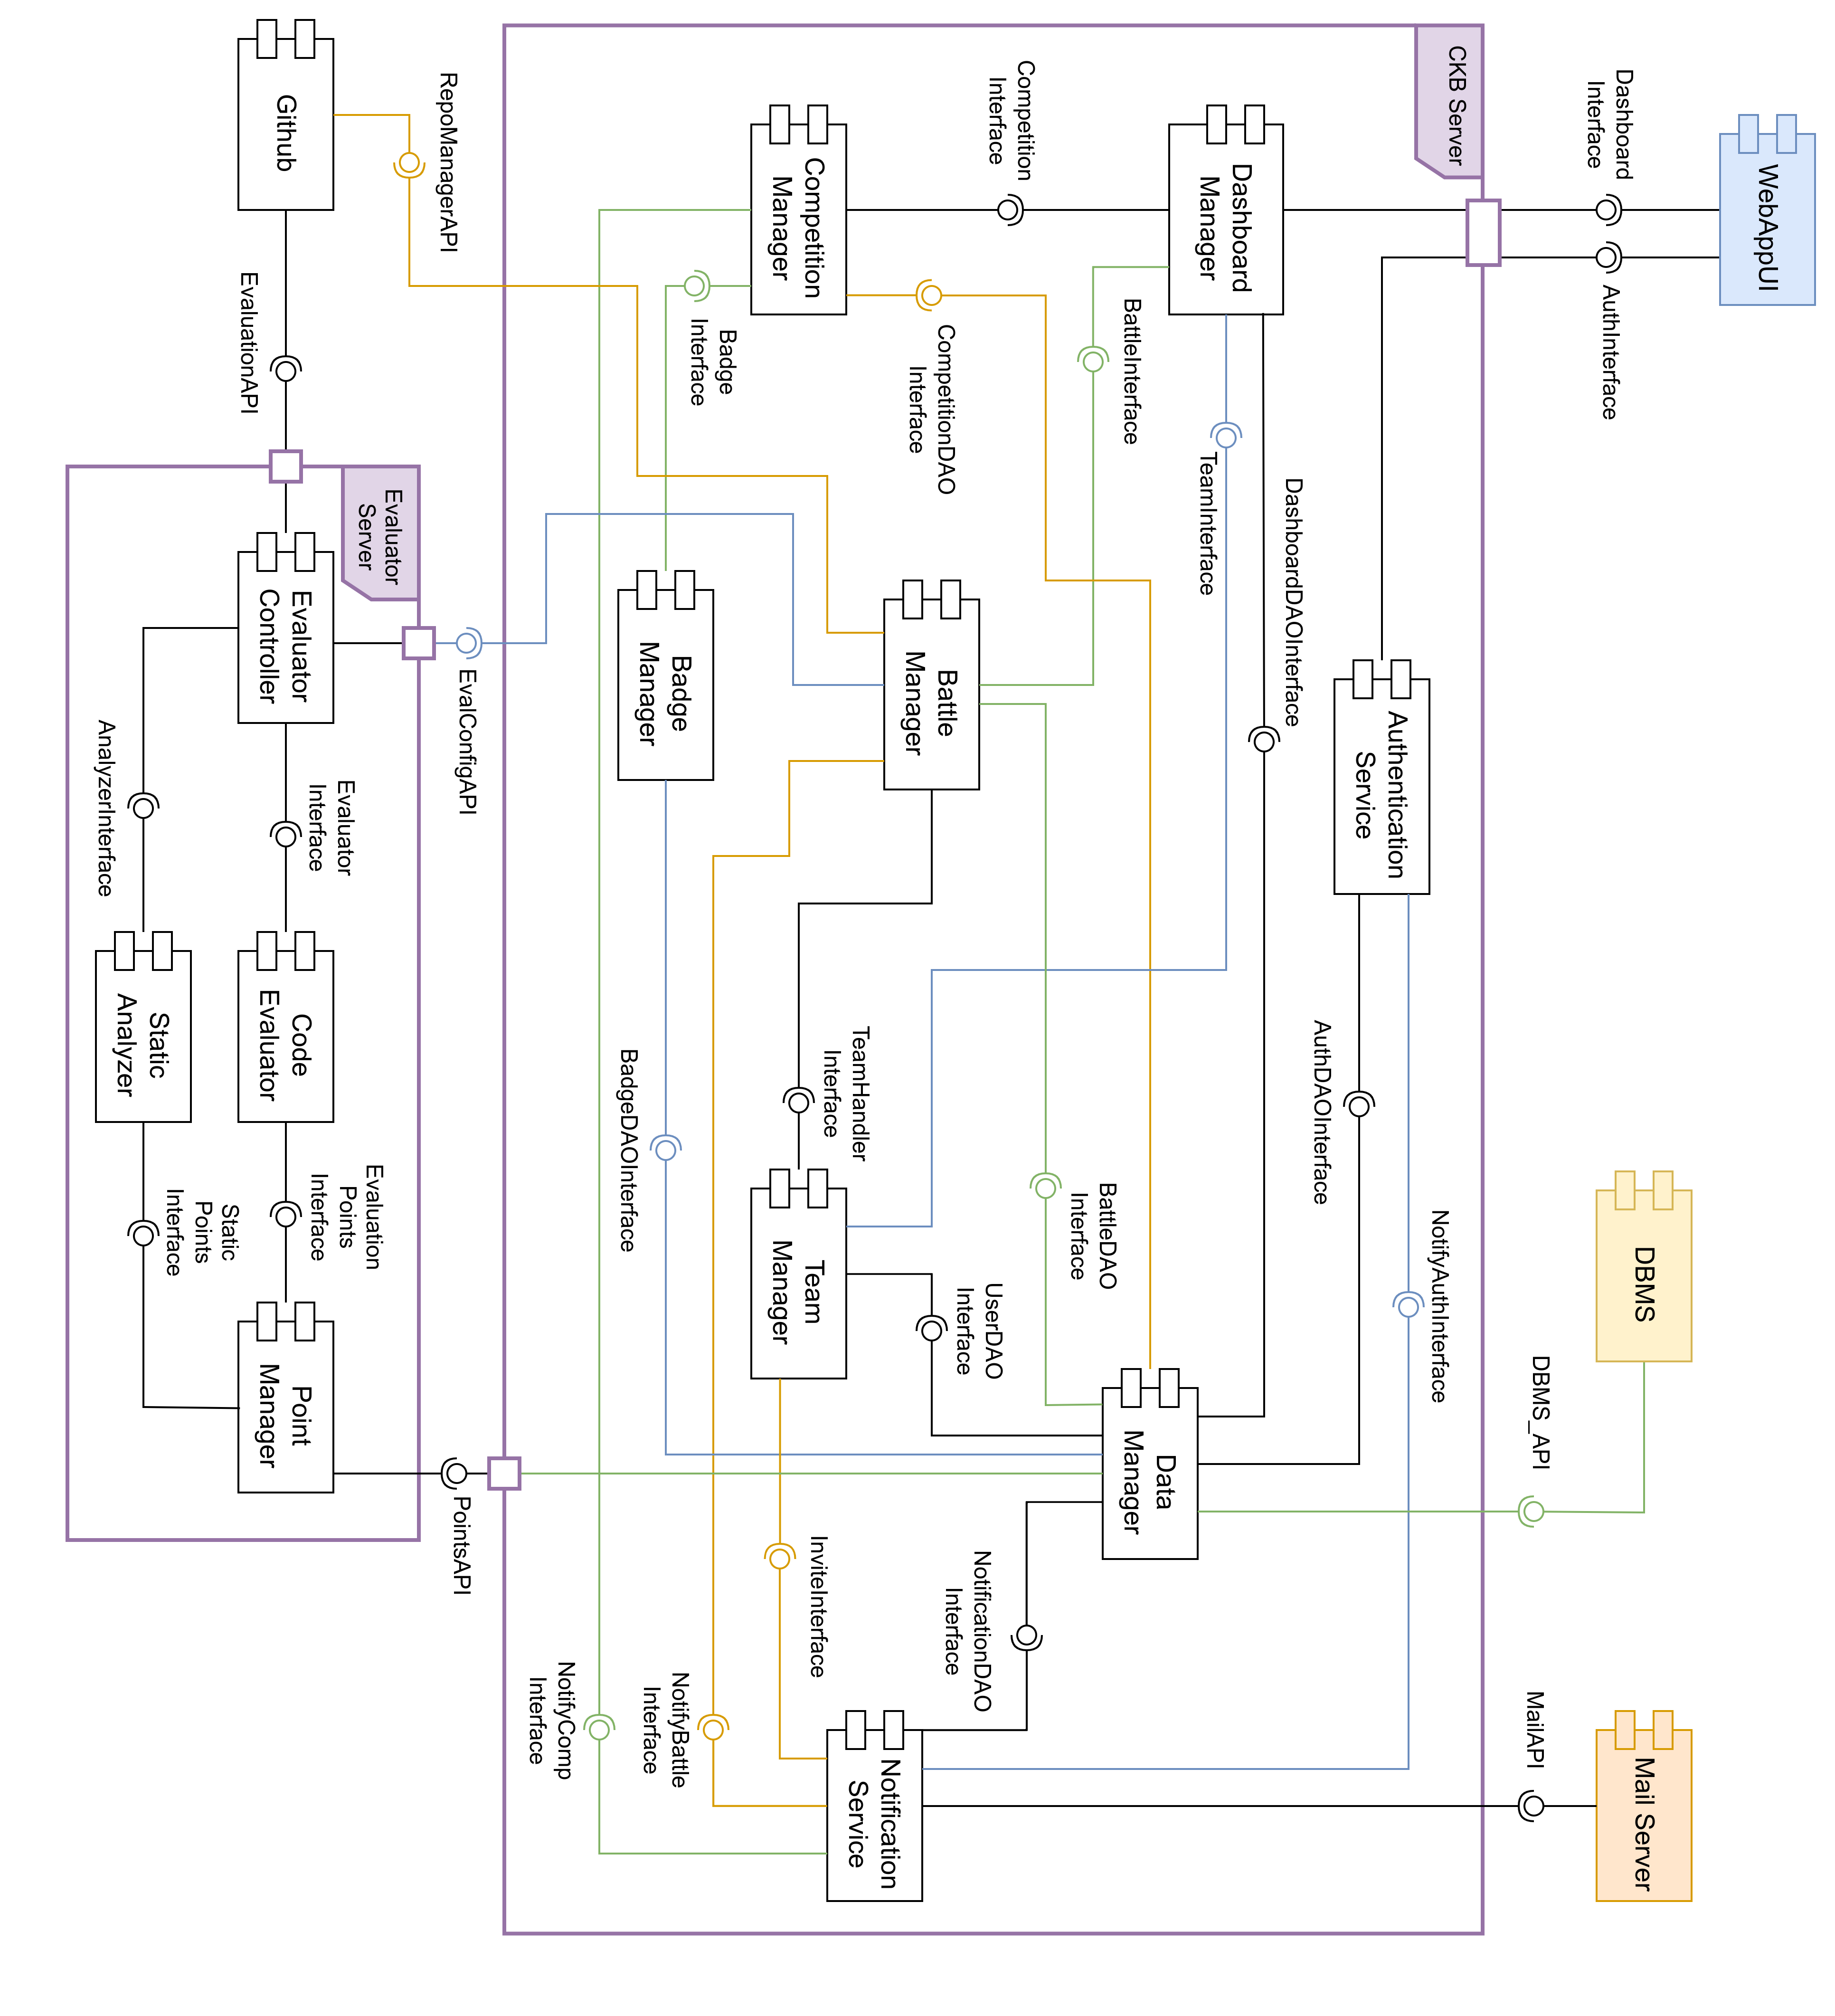
\includegraphics[width=\textwidth, keepaspectratio]{ArchitecturalDesign/componentView.png}
    \caption{Deployment view}
\end{figure}
\newpage

\section{Deployment view}
\label{s:deployment-view}%

The following diagram shows the deployment view of the system. It illustrates the distribution of the components of the system on the different nodes and how they communicate bewteen them. The system is composed by four tiers: the client tier, the application tier, the data tier and the evaluation tier. The client tier is composed by the web browser, which is used by the users to access the application. The application tier is composed by the application servers, which are used to handle the requests from the users and to communicate with the database and with the evaluation servers. The data tier is composed by the database, which is used to store the data of the application. The evaluation tier is composed by the evaluation servers, which include both the static analyzer and the code evaluator.

\begin{figure}[H]
    \label{fig:deployment-view}
    \centering
    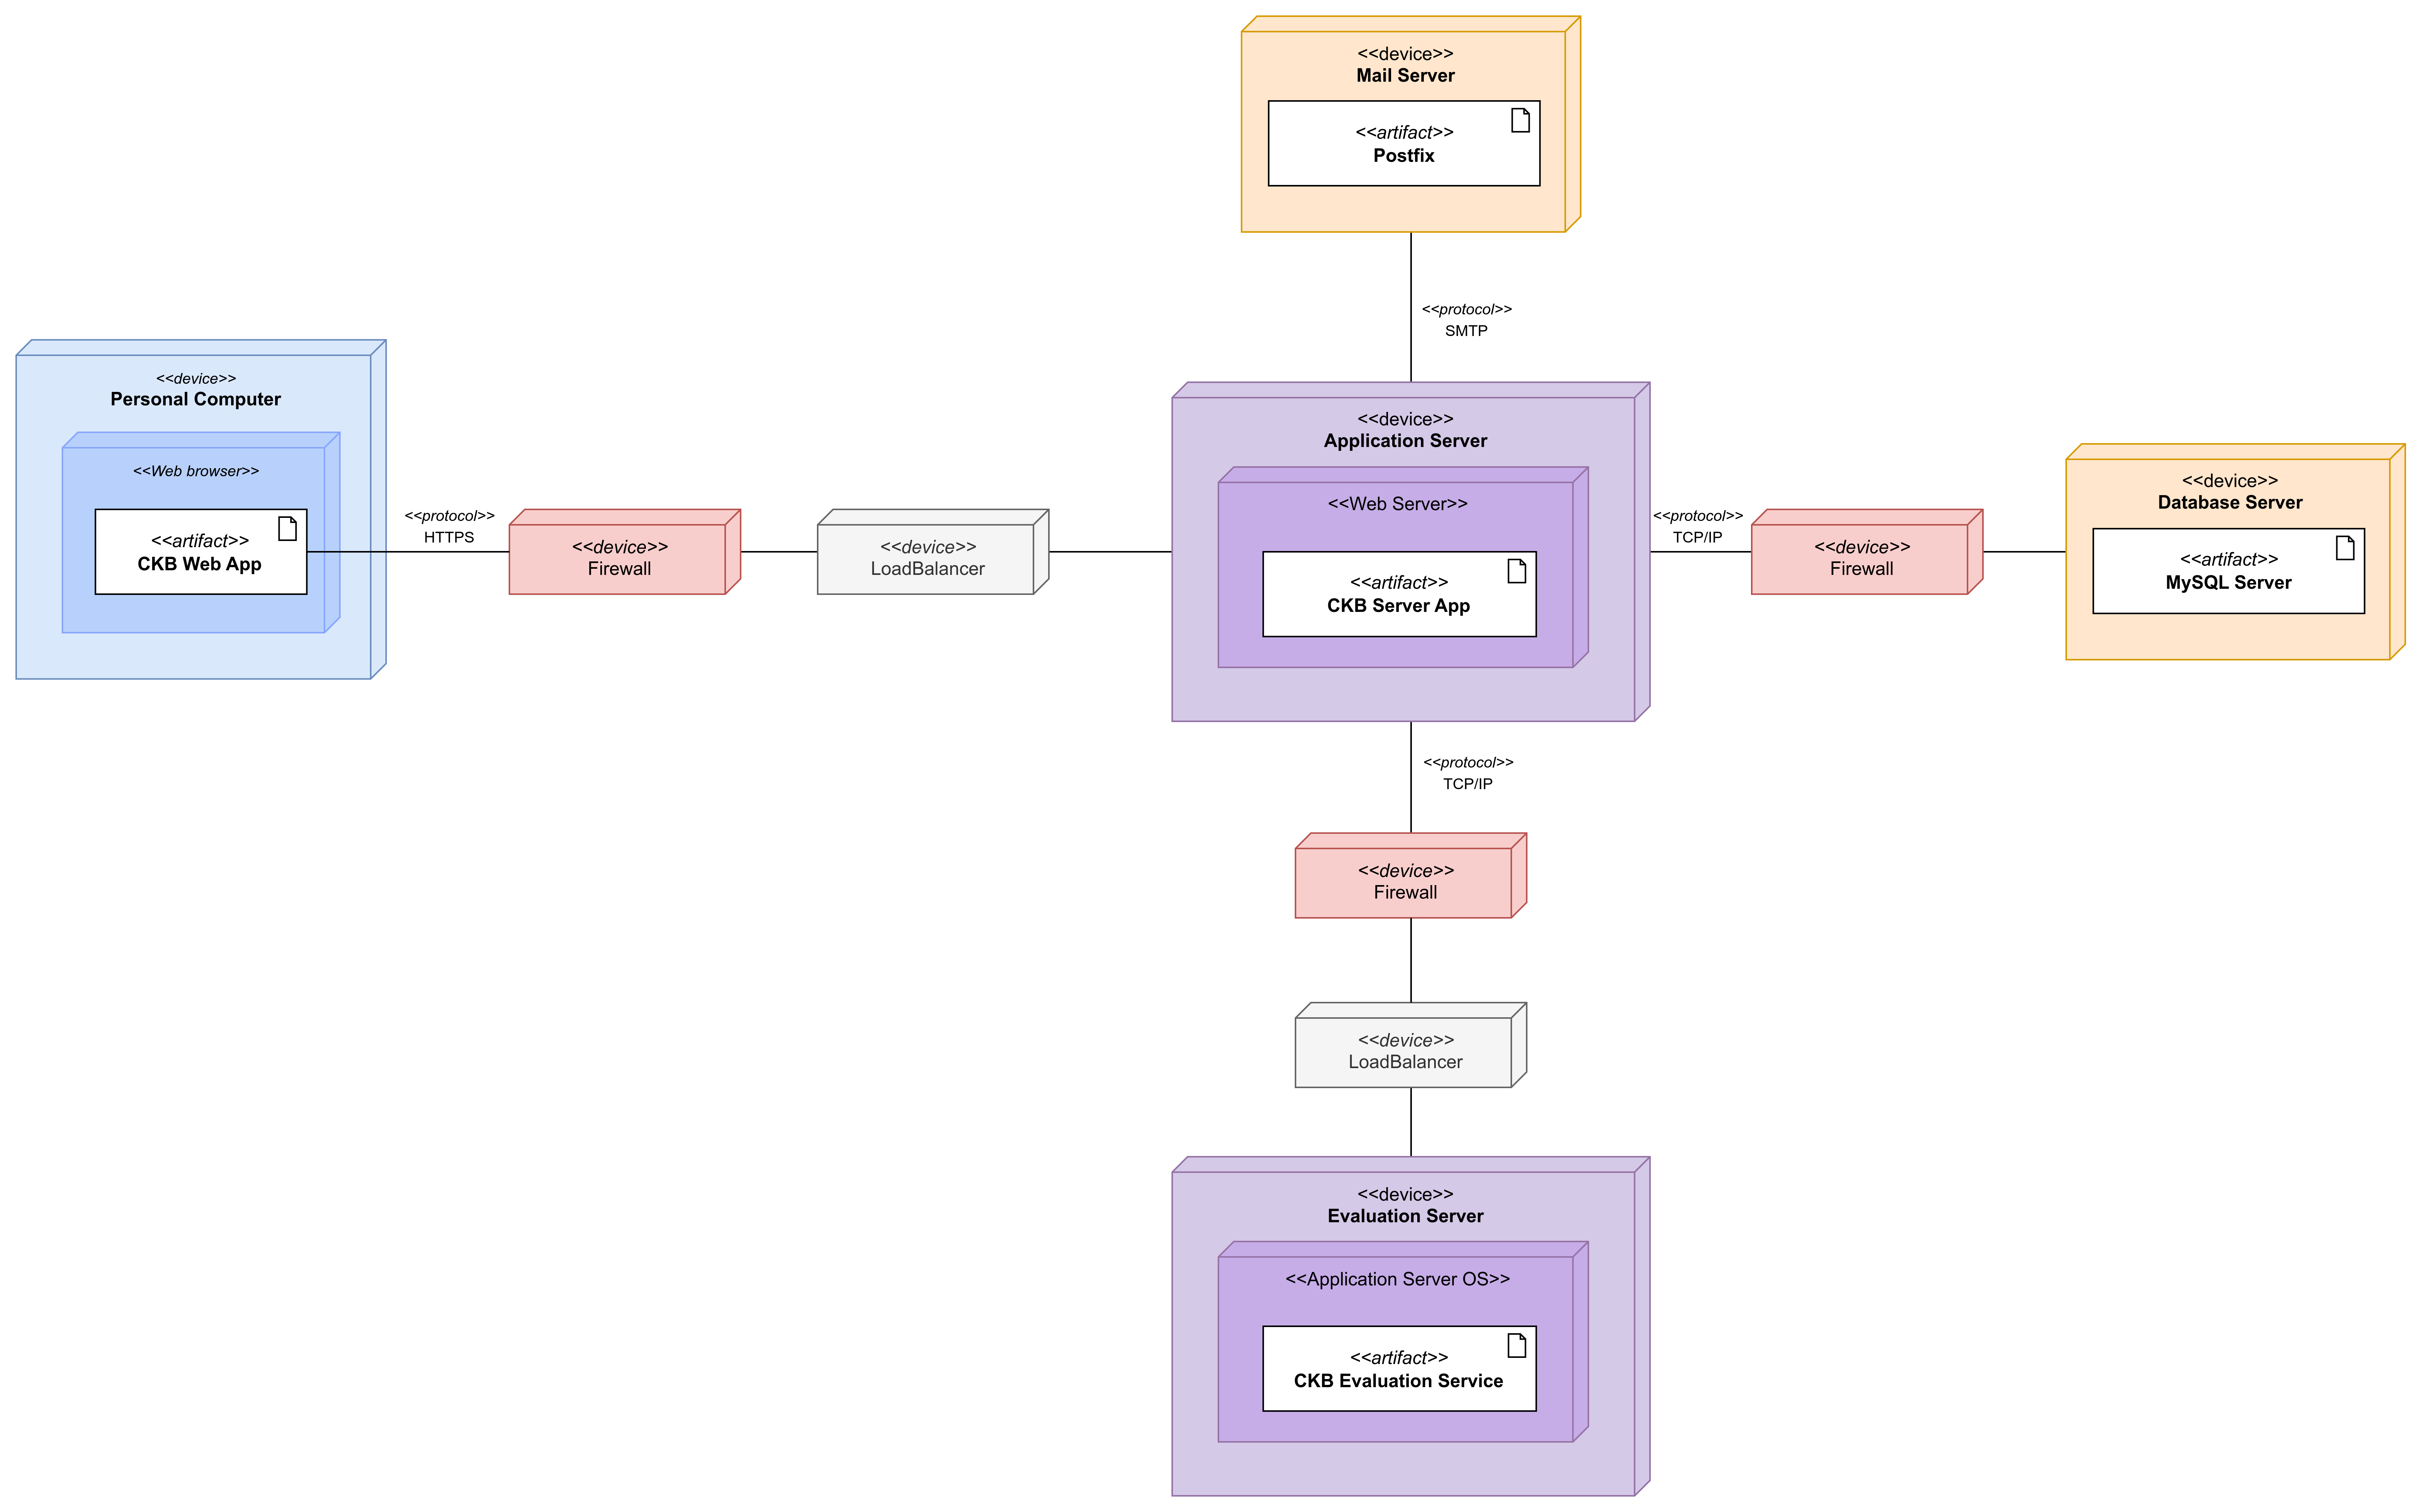
\includegraphics[width=\textwidth]{ArchitecturalDesign/deploymentView.png}
    \caption{Deployment view}
\end{figure}


\subsection{Load Balancing}
Since the CKB will be potentially have a lot of concurrent users, we decided to use a load balancer to distribute the load among multiple servers. This allows us to have a more scalable application, because we can add more servers to the system to handle the increasing load.

A load balacing is also applied for the Evaluation Servers to handle the queue of the new commits to evaluate.

\subsection{Firewall}
To protect the application from external attacks, we decided to use multiple firewall to filter the traffic. In particular, we have a firewall between the client and the load balancer, a firewall between the application servers and the load balancer before the Evaluation Server and a firewall between the application servers and the database. This allows us to have a more secure application, because the firewall will filter the traffic before it reaches the different components of the system.


\section{Runtime view}
\label{s:runtime-view}%
This section contains the sequence diagrams of the most important operations of the system. The diagrams include the component that we have already described in the previous section and the external components that are involved in the operations.

\subsubsection*{User Registration}
\label{ss:registration_diagram}%
When a user wants to register to the system, he/she has to fill in the registration form and submit it. The difference between a ST and an ED is in the information passed with \textit{UserInfo} object, where the ED has to insert also the information about the institution he/she works for.

The whole process is mainly handled by the \textit{Authentication Service} component, that interact with the \textit{Data Manager} component to validate the information and insert the new user into the DBMS.

The system will check if the information inserted are valid and if the user is not already registered. This check is done internally from CKB and if the information are valid and the user is not already registered, the system will insert it into the DBMS and sends an email to the user with a link to confirm the registration, using the \textit{Notification Manager} component. The user will click on the link and the \textit{Authentication Service} will confirm the registration.

If the information inserted are not valid, the user is already registered or the confirmation link is expired, the system will send an error message to the user.

\begin{figure}[H]
  \centering
  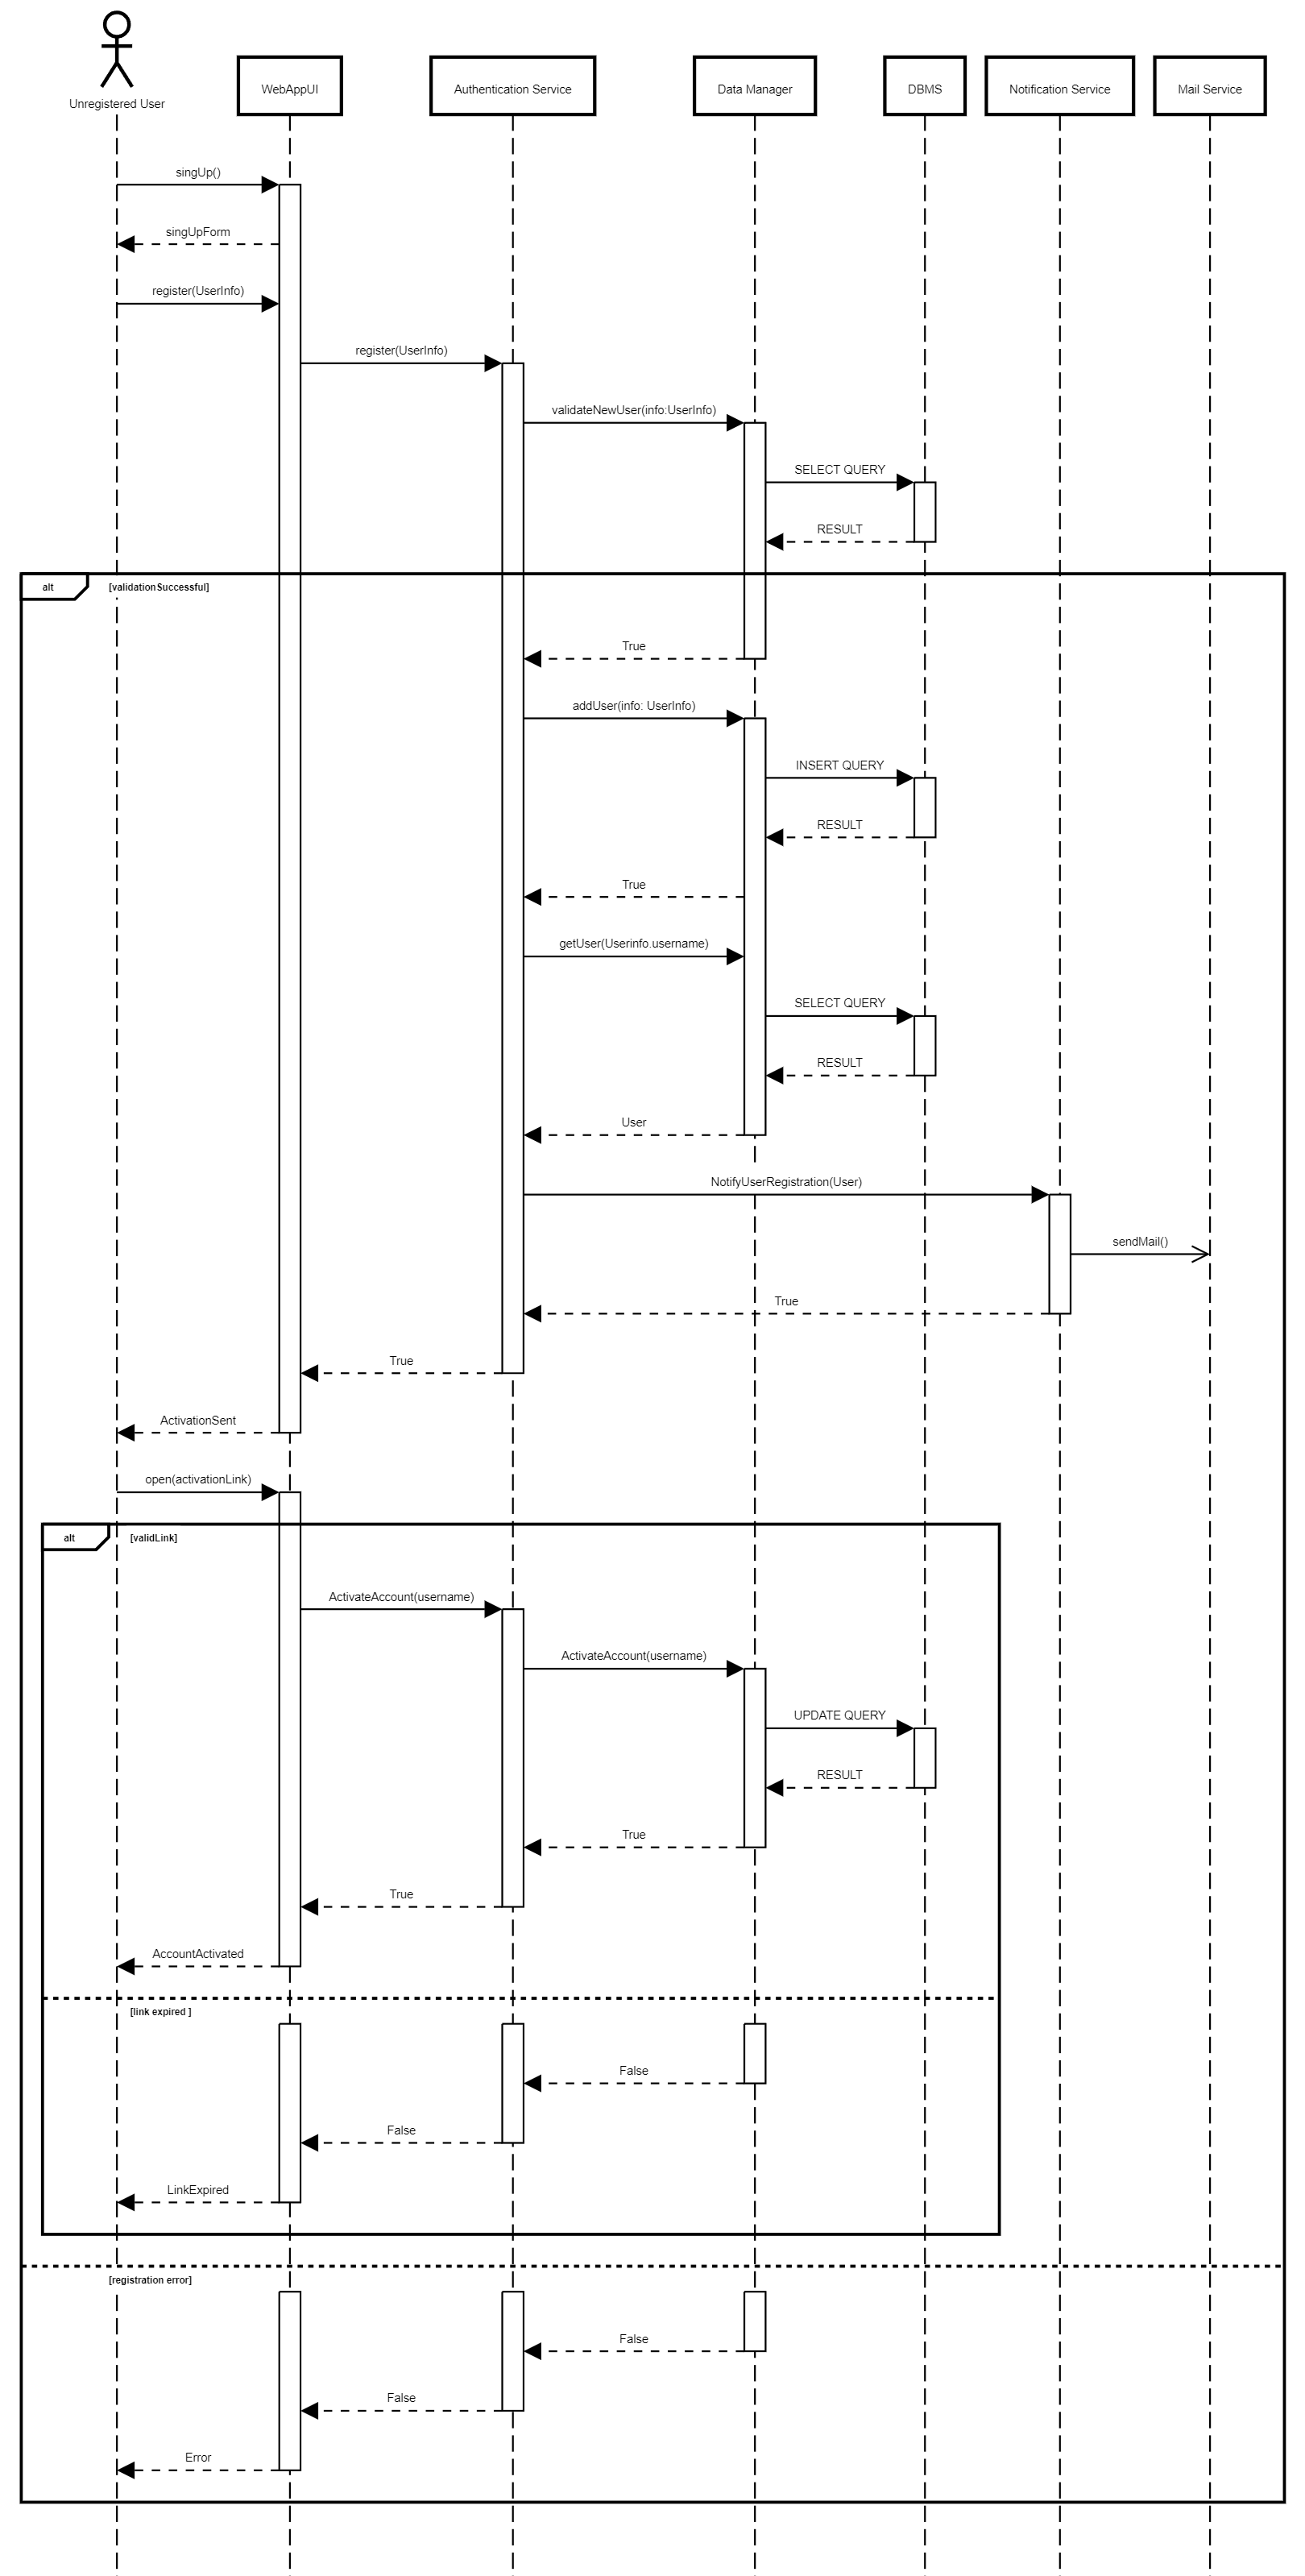
\includegraphics[width=\textwidth,height=\textheight, keepaspectratio]{SequenceDiagrams/01-UserRegistration.png}
  \caption{Registration sequence diagram}
  \label{fig:registratio_diagramn}
\end{figure}

\subsubsection*{User Login}
\label{ss:login_diagram}%
When a user wants to login to the system, he/she has to fill in the login form and submit it. This process is equal for both the ST and the ED. As the User Registration, the whole process is handled by the \textit{Authentication Service} component, that interact with the \textit{Data Manager} component to validate the information. Once the user is logged in, the \textit{Authentication Service} will generate a token for the user, send it to the client and the user can finally access the dashboard.

If the login information are not valid, the system will show an error message to the user.

\begin{figure}[H]
  \centering
  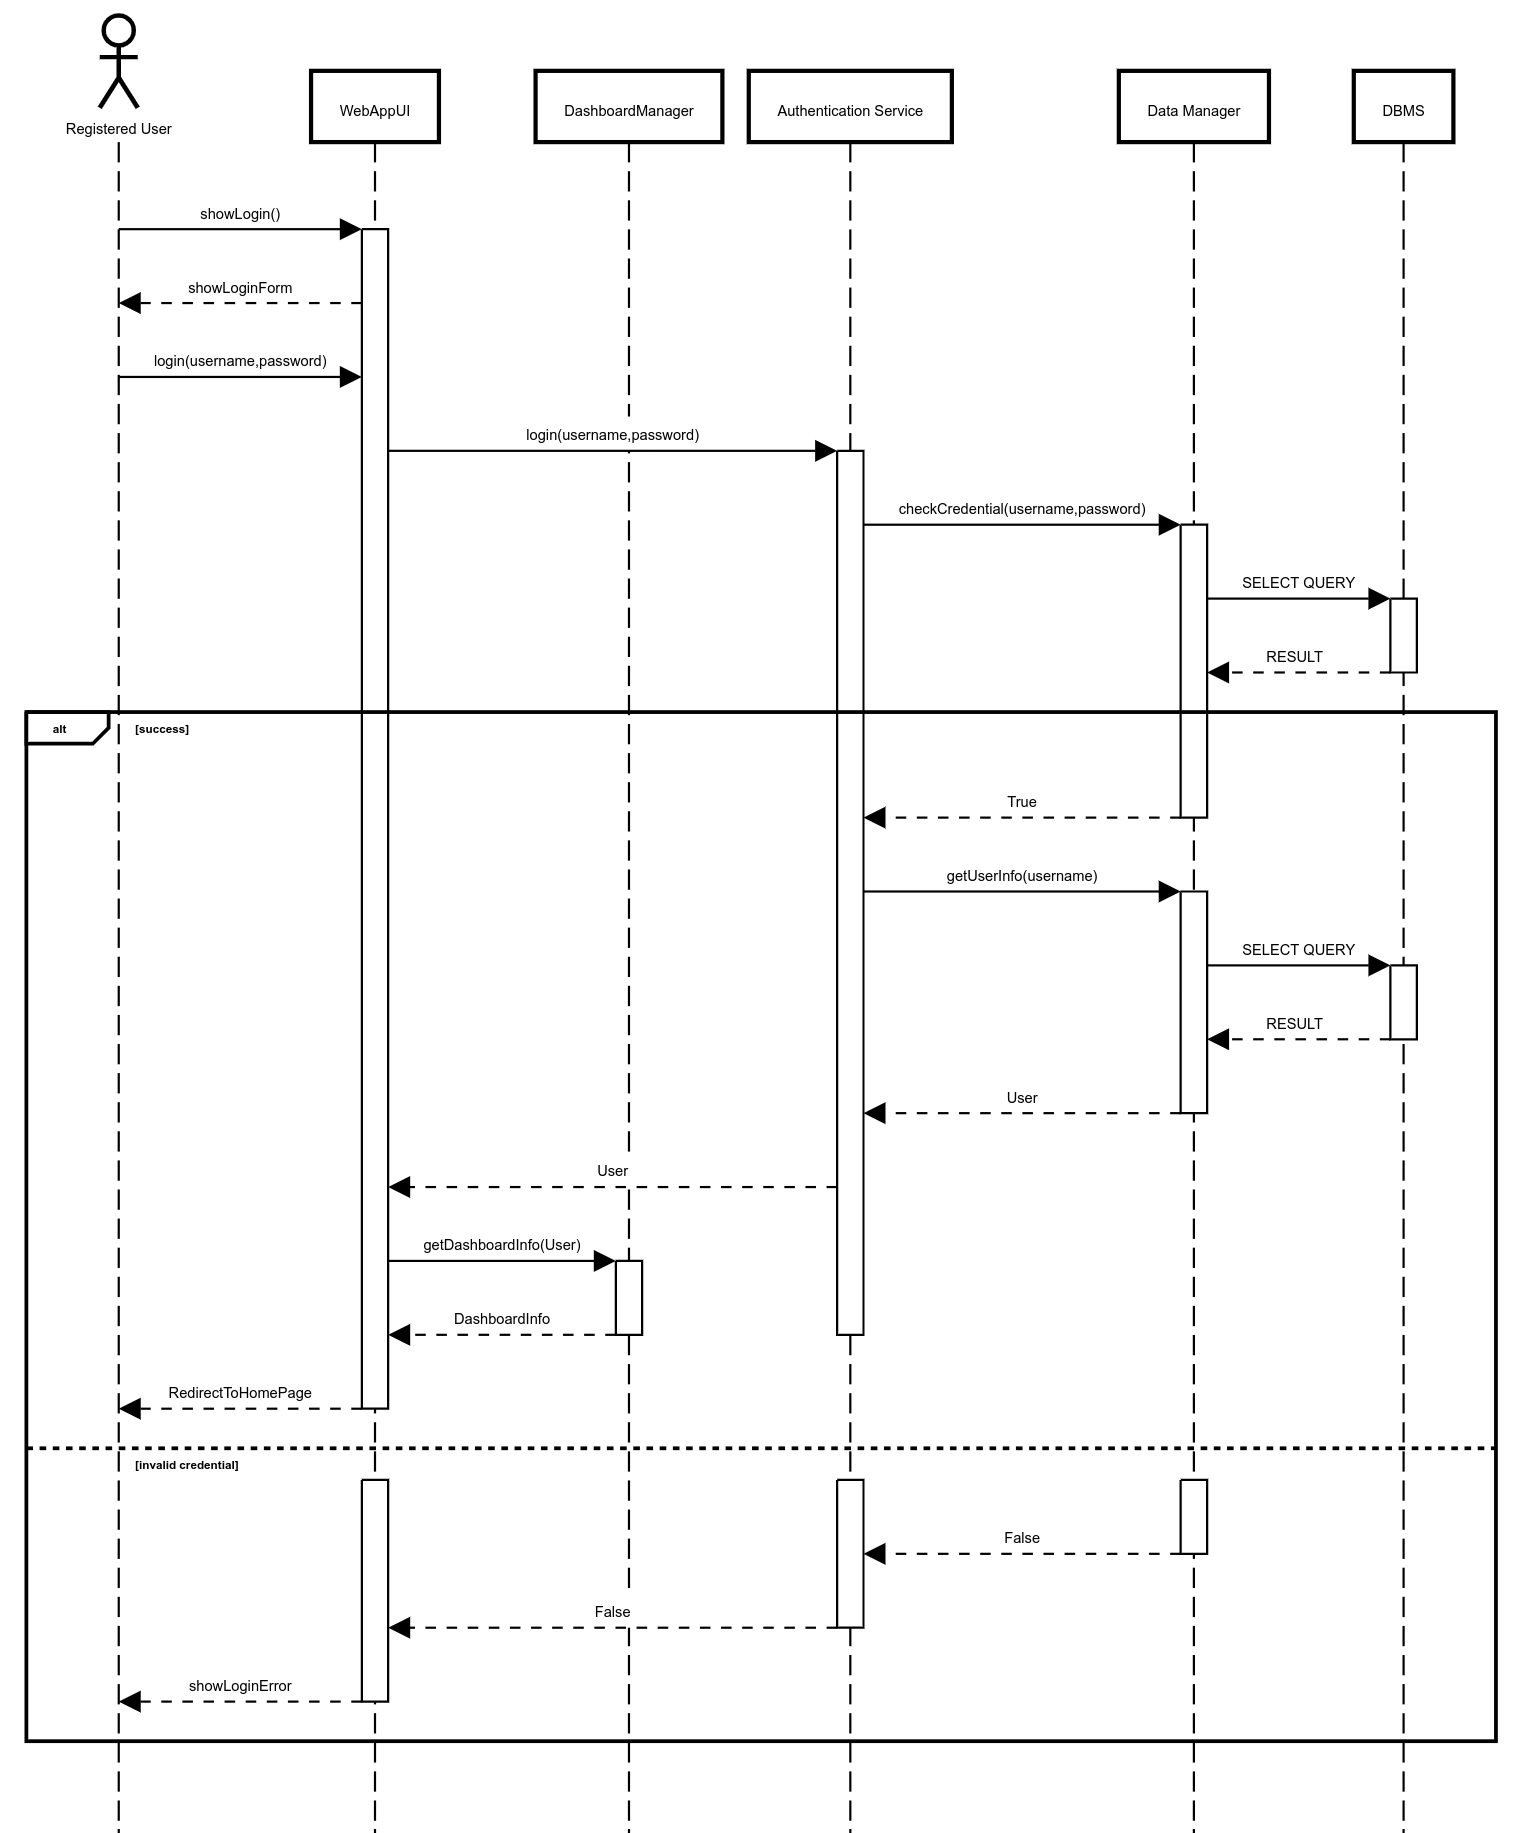
\includegraphics[width=\textwidth,height=0.7\textheight, keepaspectratio]{SequenceDiagrams/02-UserLogin.png}
  \caption{Login sequence diagram}
  \label{fig:login_diagramn}
\end{figure}

\subsubsection*{ED Creates Competition}
\label{ss:create_competition_diagram}
Here is shown how a competition is created by an ED. The ED has to fill in the form with the information about the competition and submit it. The \textit{Competition Manager} component will check if the name is available and if so the competition will be created and inserted into the DBMS using the \textit{Data Manager} component, otherwise a new name will be requested. The system will then returns the competition and will be shown the competition page.

\begin{figure}[H]
  \centering
  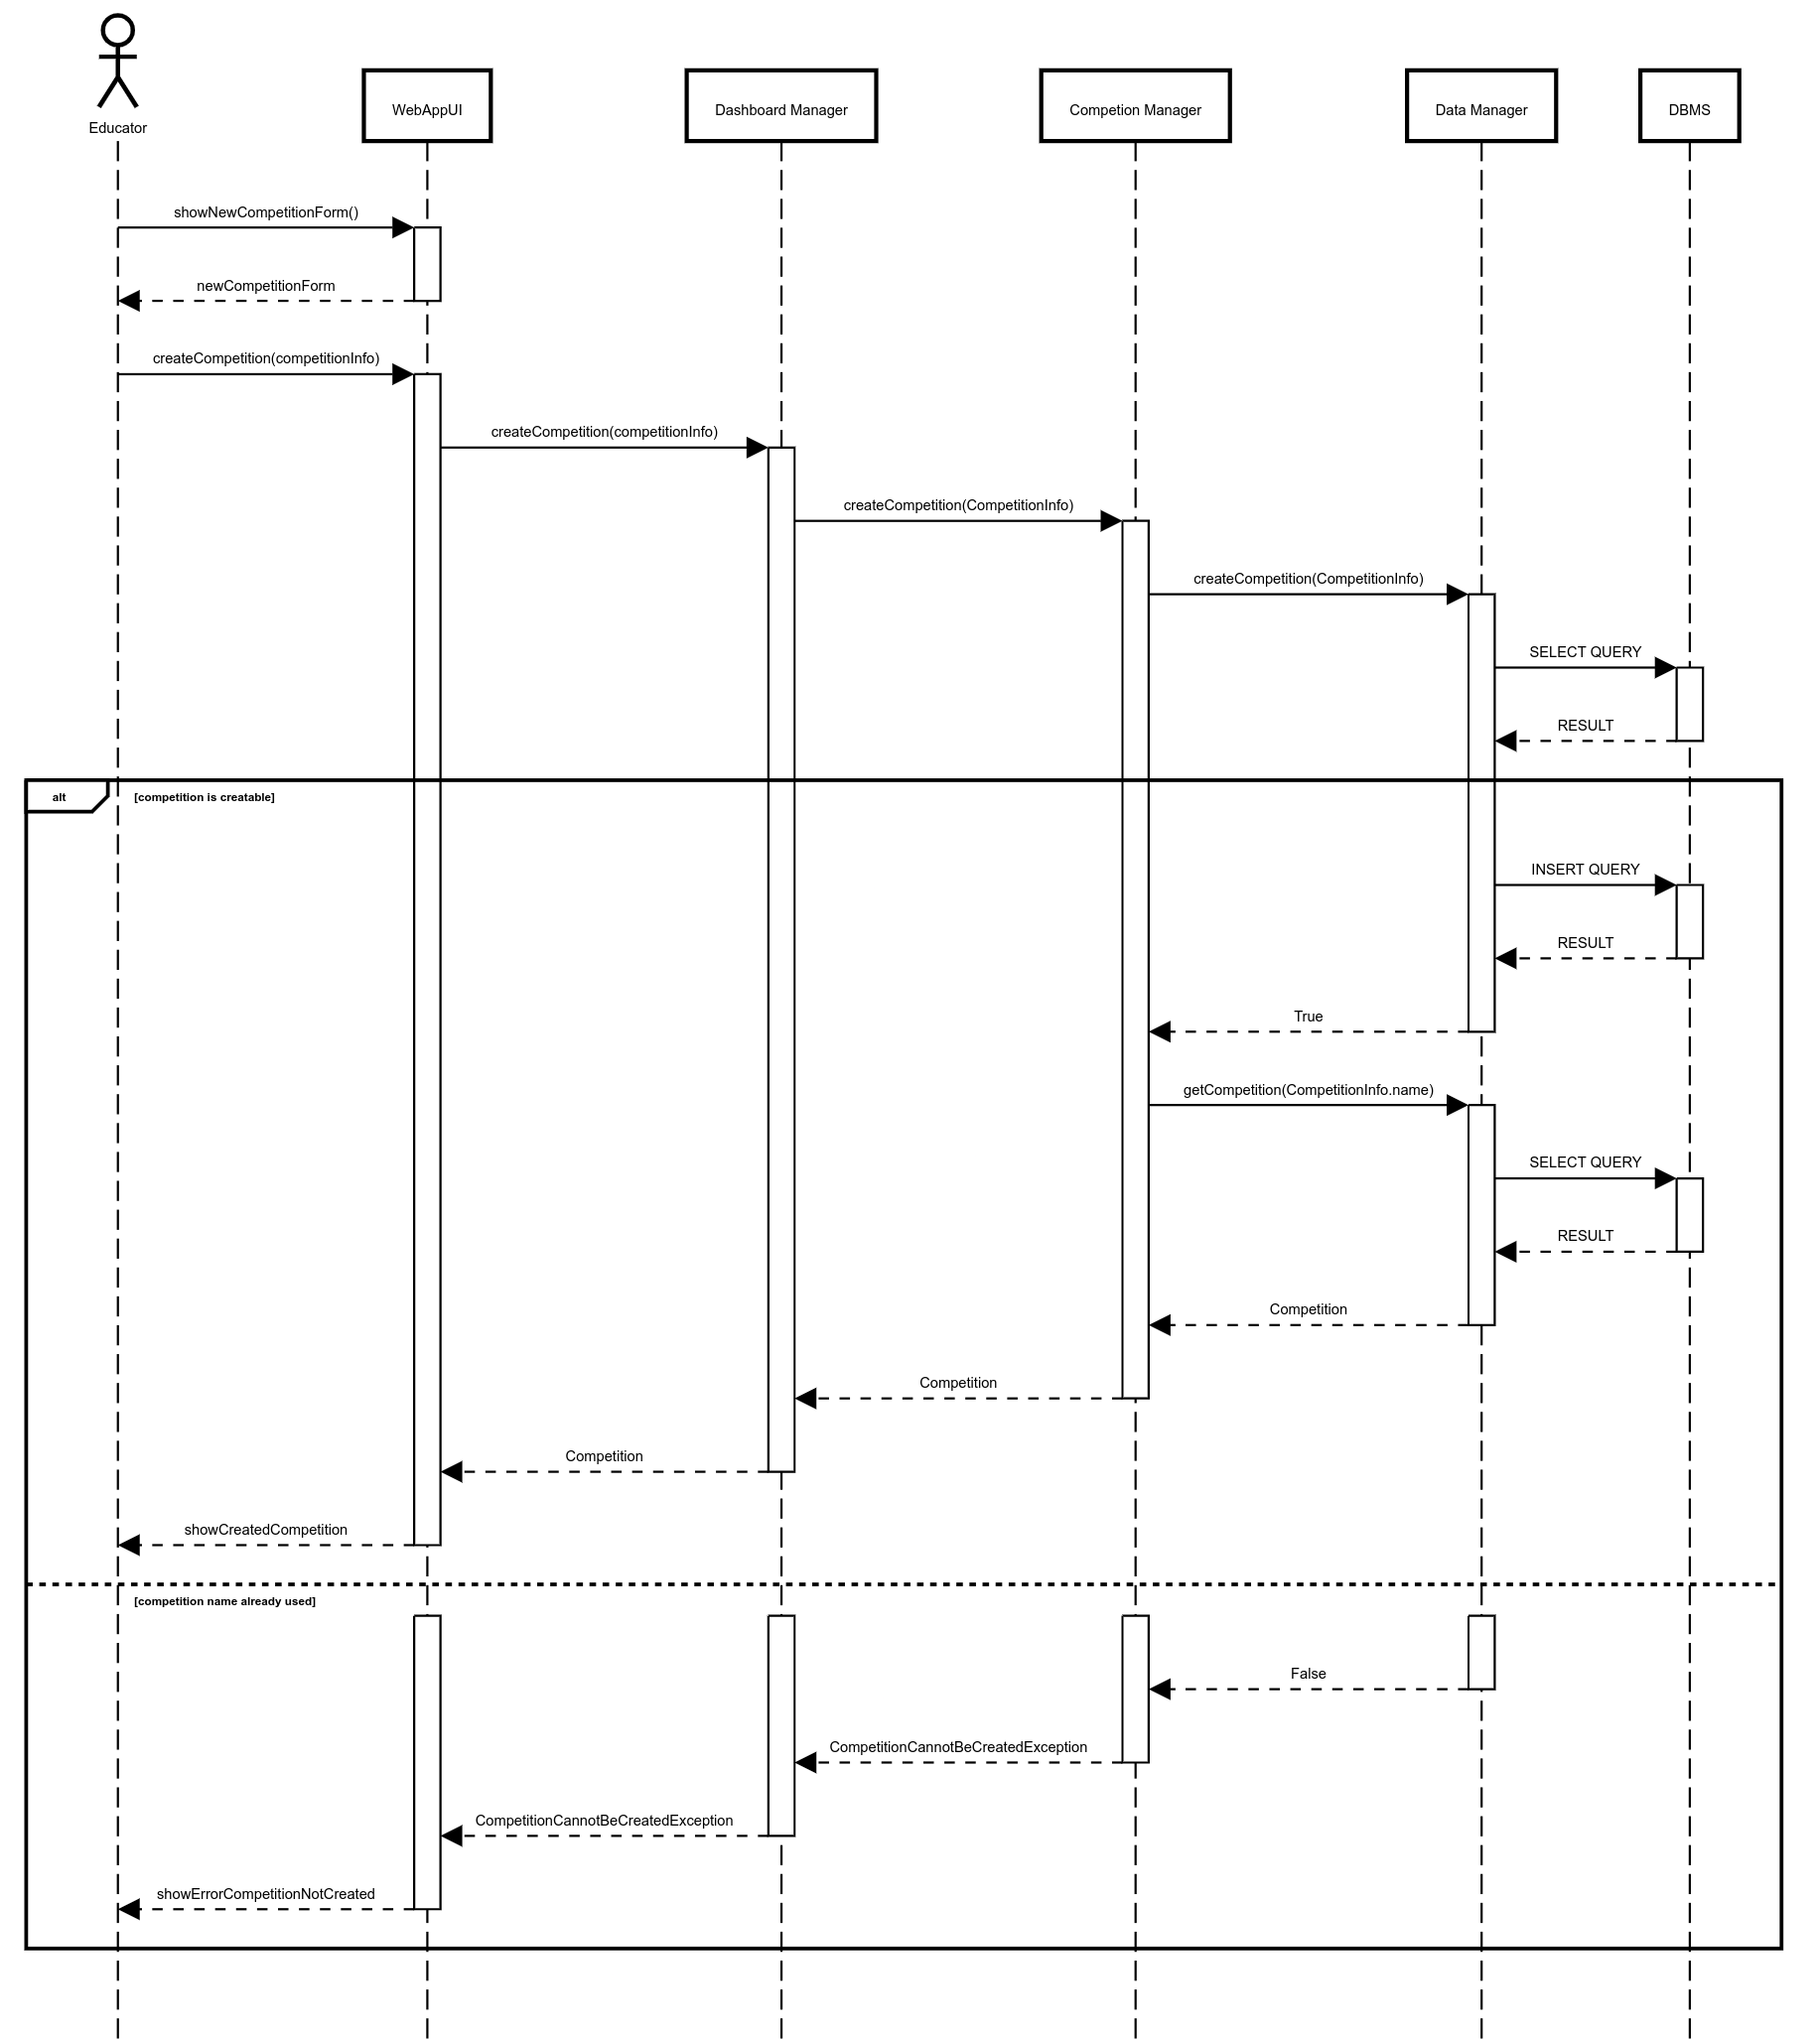
\includegraphics[width=\textwidth,height=0.74\textheight, keepaspectratio]{SequenceDiagrams/04-EducatorCreatesCompetition.png}
  \caption{Create competition sequence diagram}
  \label{fig:create_competition_diagramn}
\end{figure}

\subsubsection*{ST Joins Competition}
\label{ss:join_competition_diagram}
The ST firstly visualize all the available competitions in the platform, then he/she can choose one of them and join it. The \textit{Competition Manager} component will handle both the search of the available competitions and the insertion into the DBMS using the \textit{Data Manager} component. The system will then show a success message to the user.

\begin{figure}[H]
  \centering
  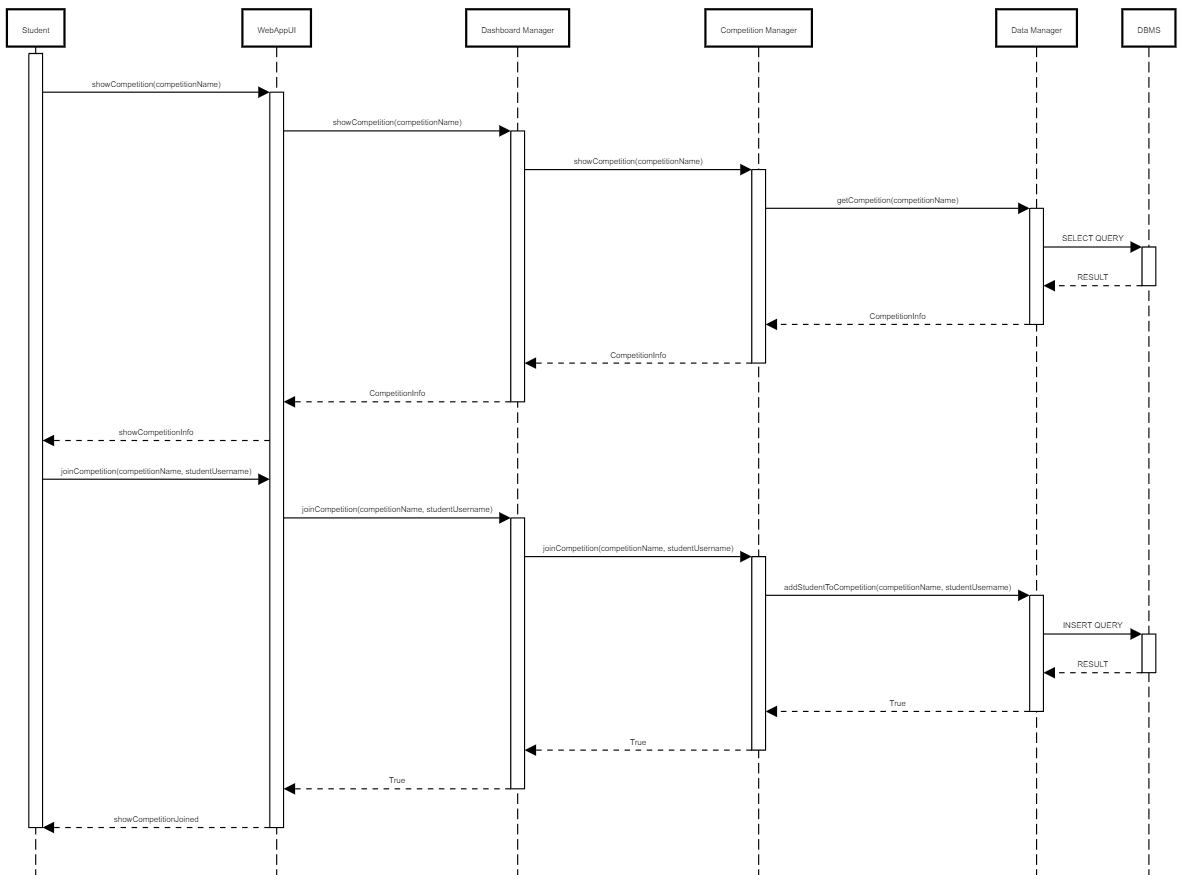
\includegraphics[width=\textwidth,height=\textheight, keepaspectratio]{SequenceDiagrams/05-StudentJoinCompetition.png}
  \caption{Join competition sequence diagram}
  \label{fig:join_competition_diagramn}
\end{figure}

\subsection*{ED Creates Battle}
\label{ss:create_battle_diagram}
When a ED wants to create a battle, he/she needs to be in a competition page that he/she manages. The interaction is divided in two parts: the first one is where the ED inserts the general information about the battle, the name is then validated by the \textit{Battle Manager} component and if it is valid the system will show the second part of the form where the ED can insert the information about the automatic evaluation and static analysis. The \textit{Battle Manager} component will check if the information are valid and if so the battle will be created and inserted into the DBMS using the \textit{Data Manager} component.

If the battle is successfully created, the system will send a notification, through the \textit{Notification Manager} to all the ST enrolled in the competition where the battle has been created.

\begin{figure}[H]
  \centering
  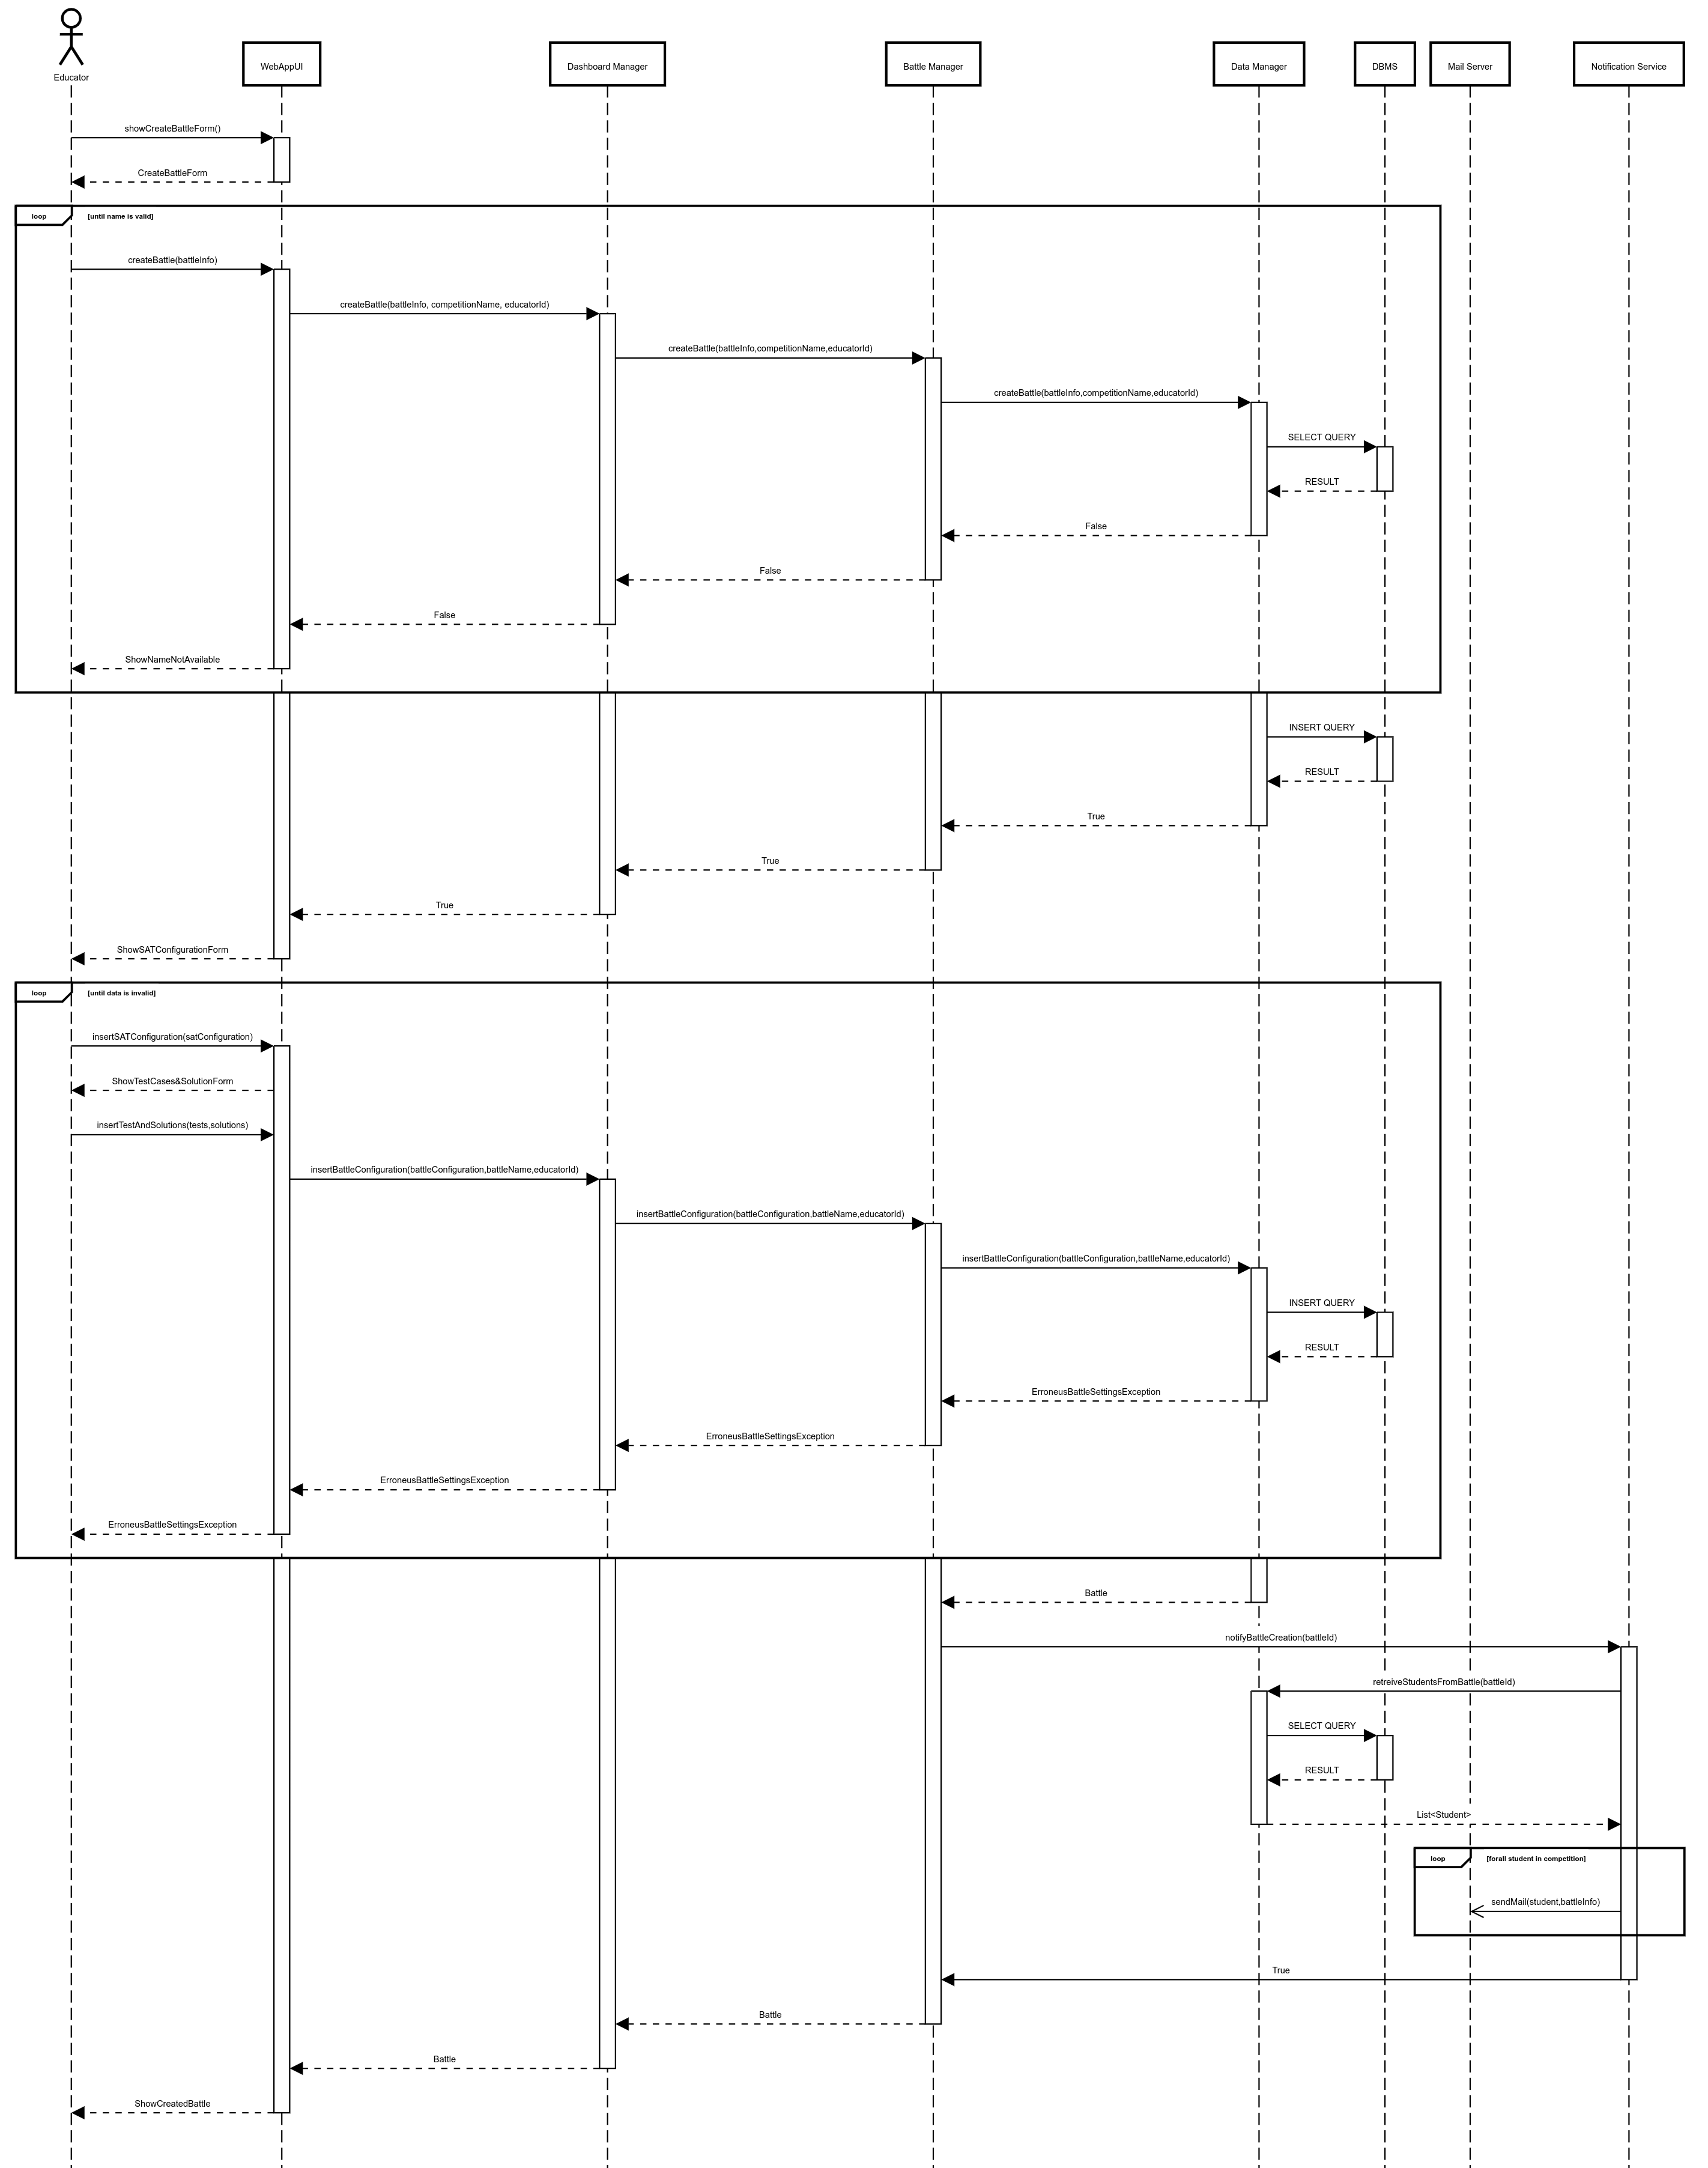
\includegraphics[width=\textwidth,height=0.83\textheight, keepaspectratio]{SequenceDiagrams/06-EducatorCreatesBattle.png}
  \caption{Create battle sequence diagram}
  \label{fig:create_battle_diagramn}
\end{figure}

%9
\subsection*{ST Joins Battle}
To be able to join a battle, a \textit{ST} must be enrolled in a competition and in such competition there has to be at least 1 battle available (subscription deadline not expired). Assuming all those things, when a ST wants to join a battle, he/she has two options: create a team (with the possibility, if enabled by the EDs of the battle, to be a singleton) or to join an already existing team. In the first case the ST has to provide the system all the information needed for the team registration, and if the team has been created correctly he/she can invite other STs to join his/her team (if the ST, owner of the team, wants to participate alone he/she must skip the invite part). In the latter case instead, the ST looks at the list of existing and available teams and if he/she wants to join one of those team they can simply click on the join button.

Since the sequence diagram below was pretty long we decided to split it in two so that it was easier to read it; this means that the two following diagrams are to be understood as consecutive (the [\textit{alt 'ST wants to join an existing public T'}] fragment, in the second part of the diagram, is the [\textit{else}] of the [\textit{alt 'ST selects to create a new T'}] fragment in the first part of the diagram)


\begin{figure}[H]
  \centering
  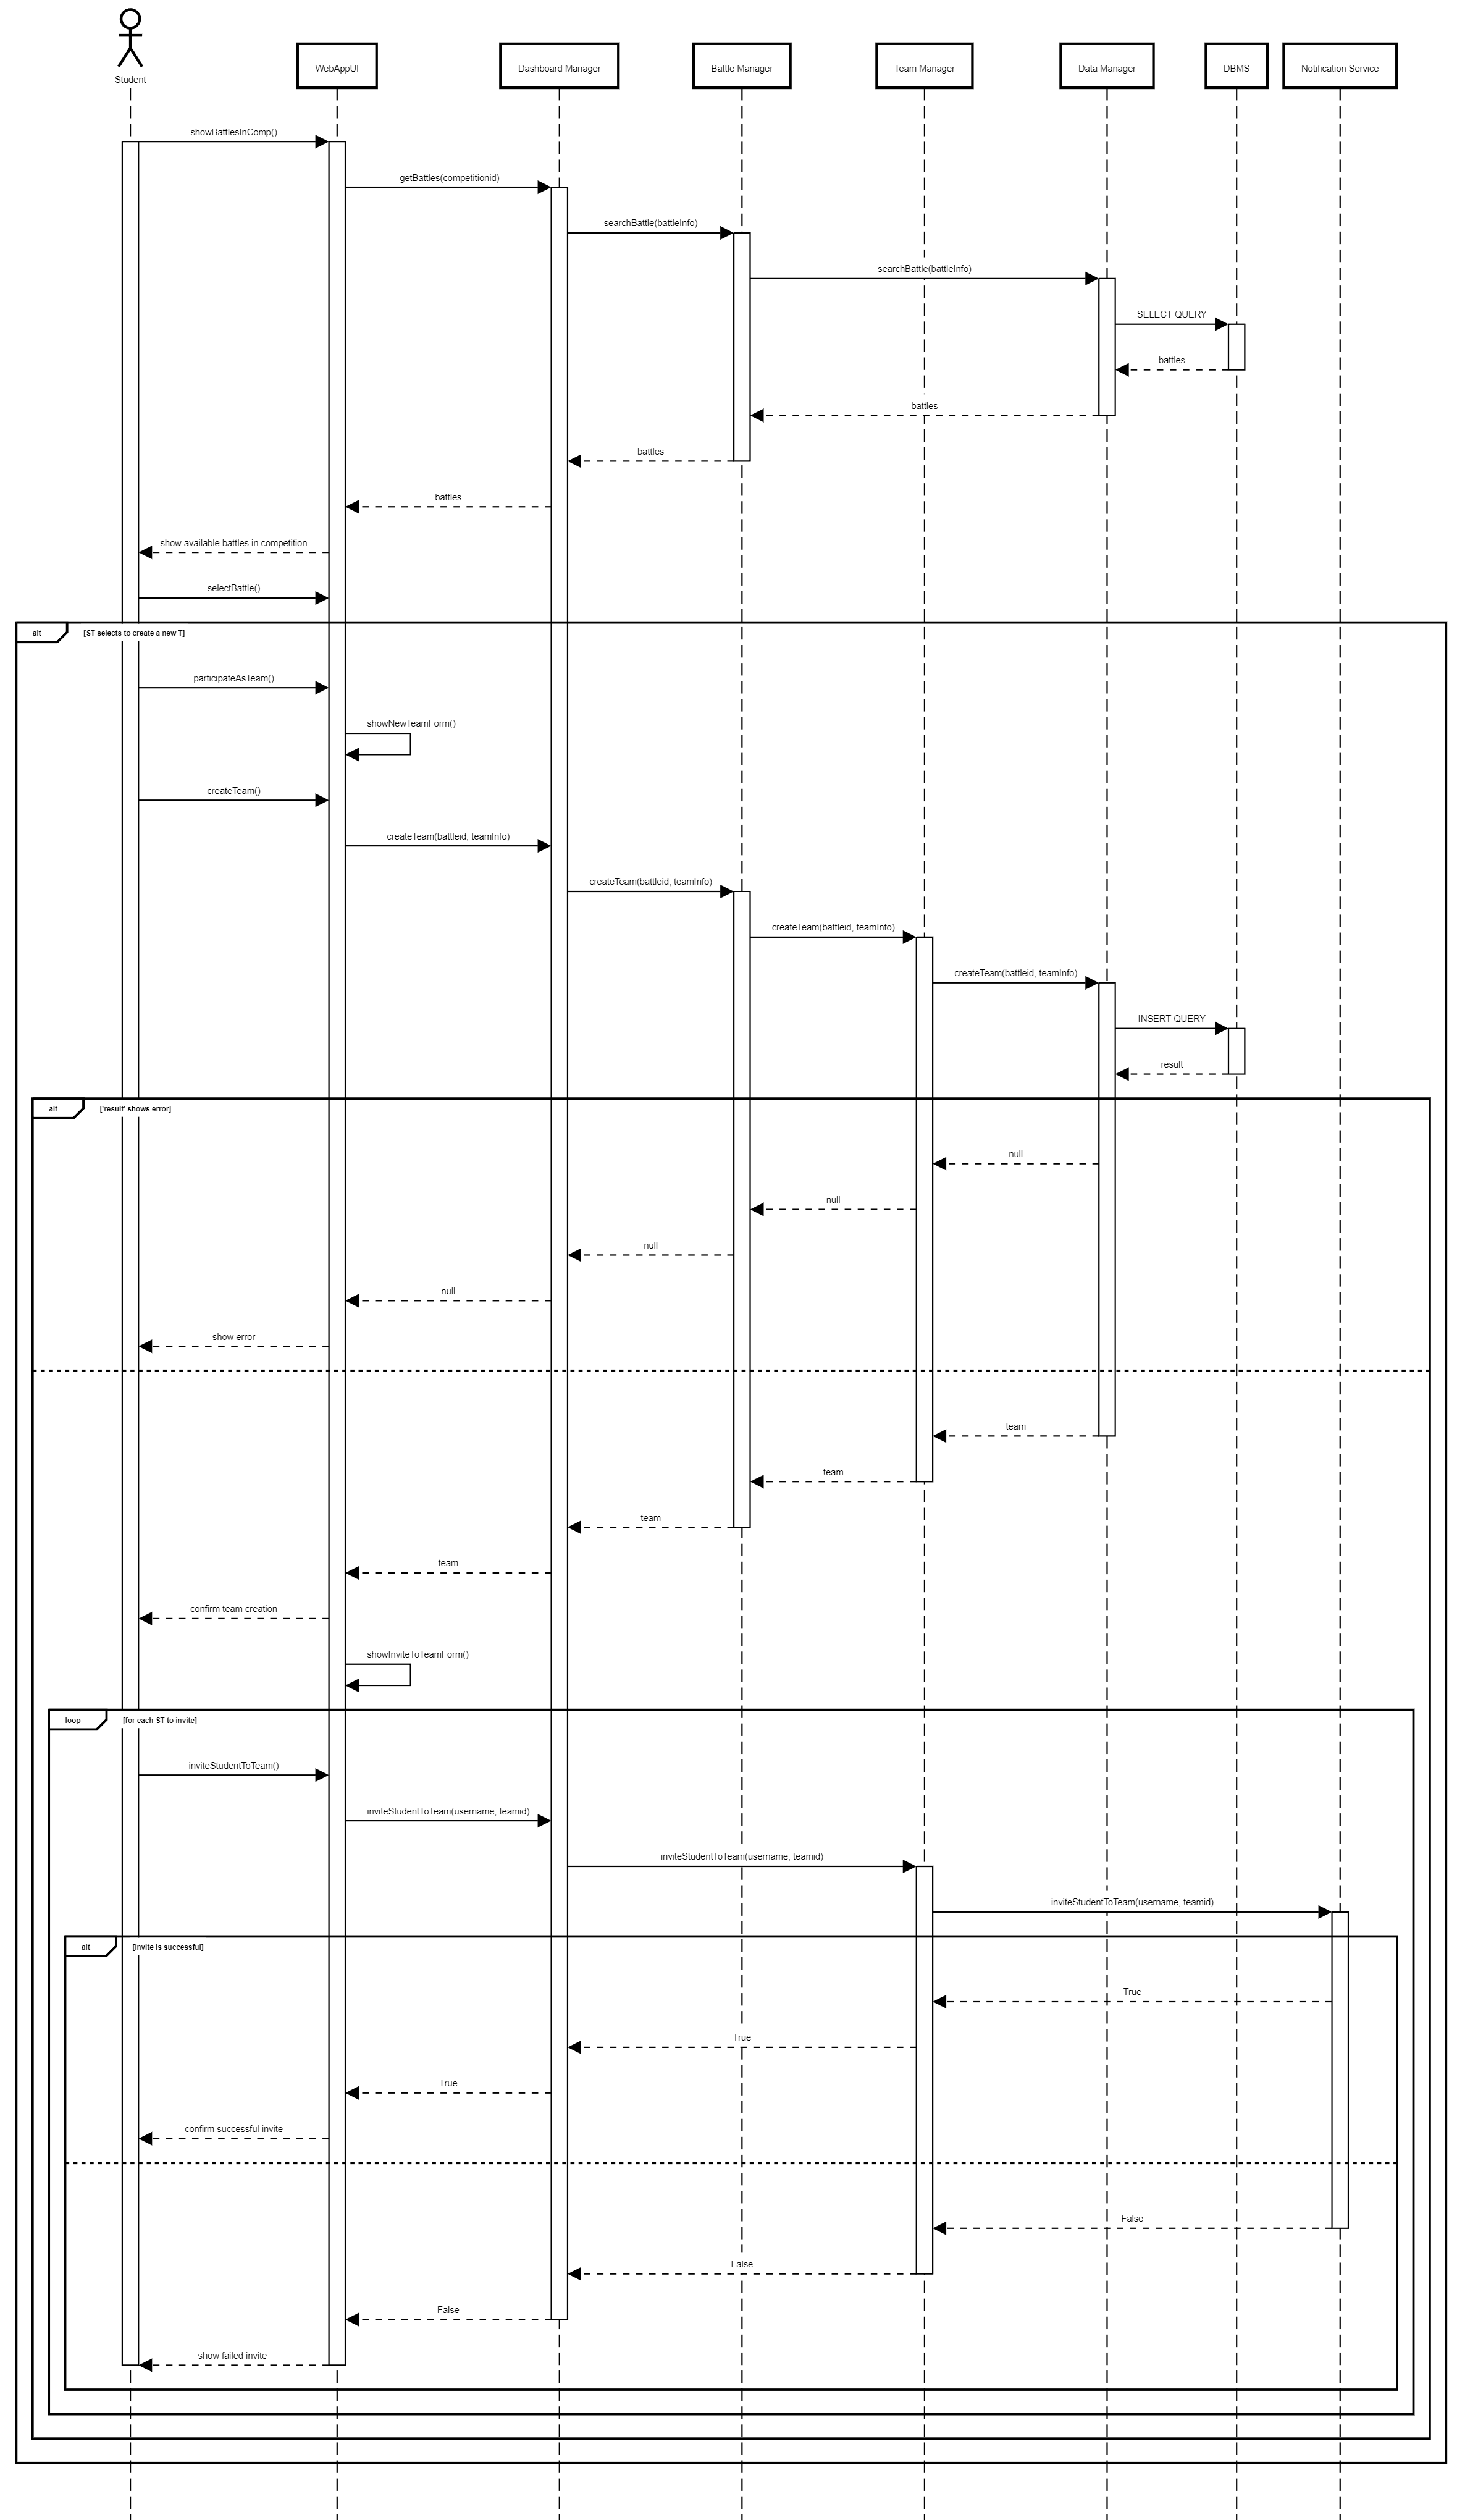
\includegraphics[width=\textwidth,height=\textheight, keepaspectratio]{SequenceDiagrams/09.1-StudentJoinsBattle.png}
  \caption{ST joins battle sequence diagram - Part 1}
  \label{fig:st_joins_battle_1}
\end{figure}

\begin{figure}[H]
  \centering
  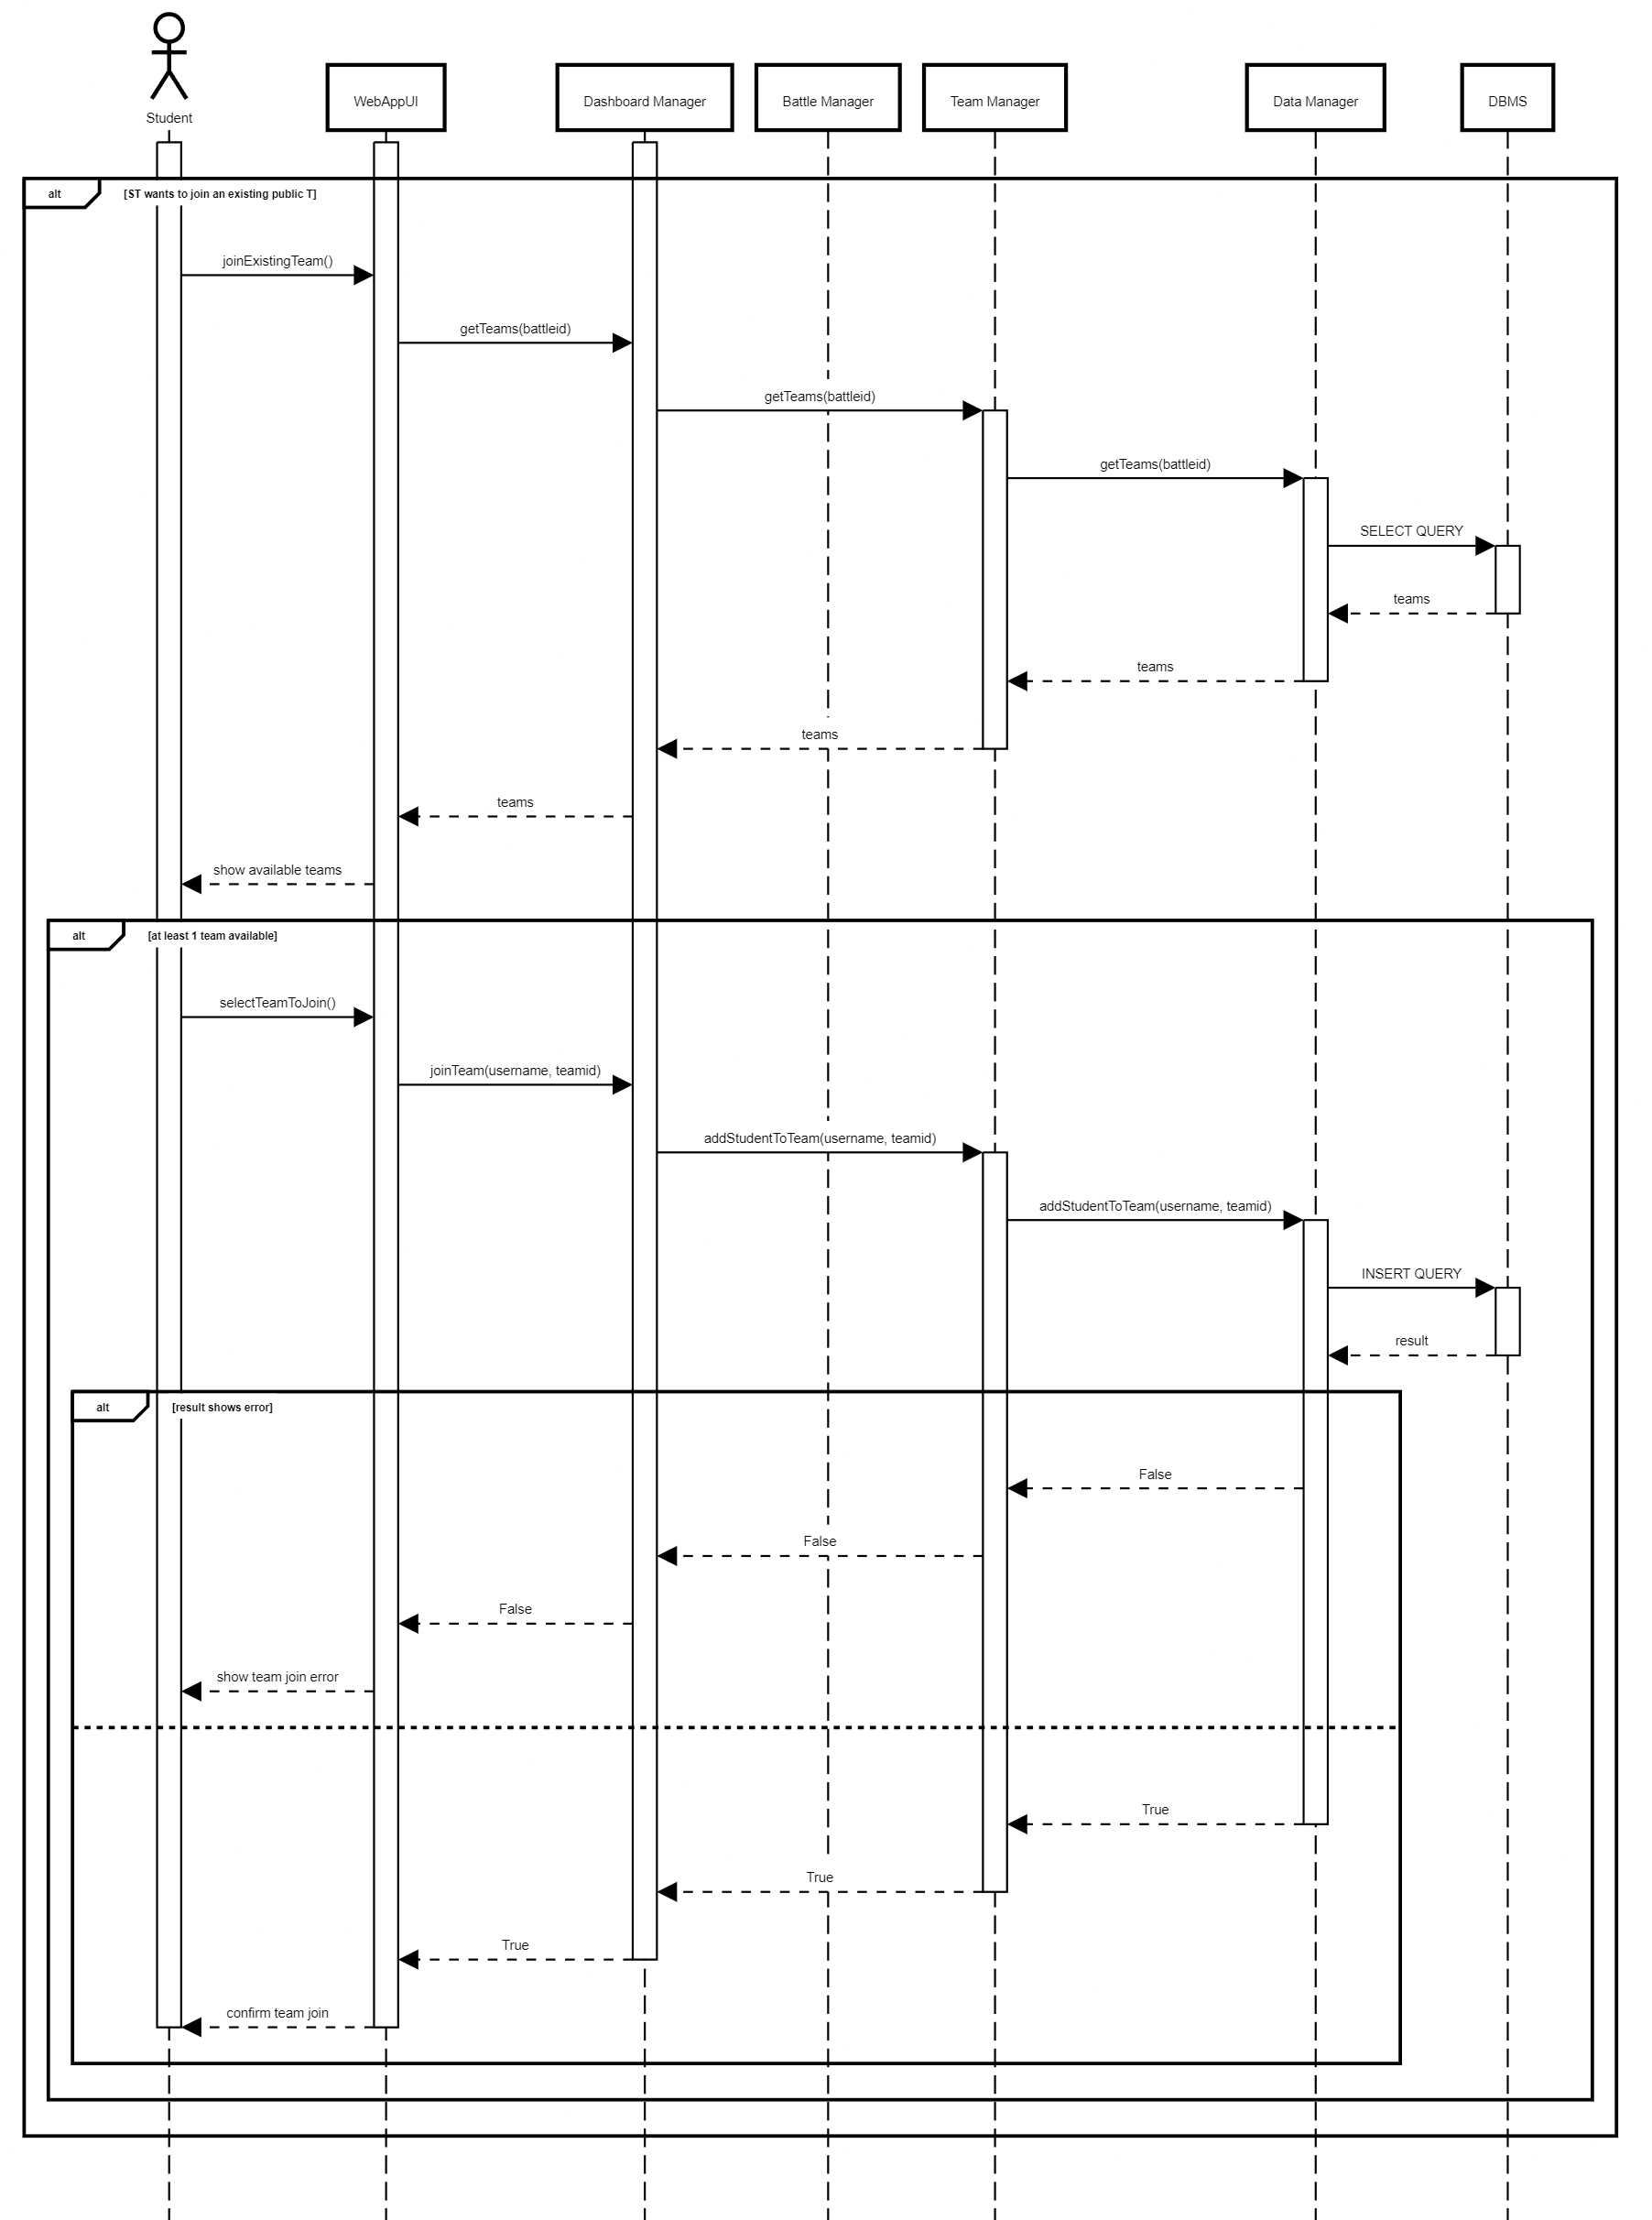
\includegraphics[width=\textwidth, keepaspectratio]{SequenceDiagrams/09.2-StudentJoinsBattle.png}
  \caption{ST joins battle sequence diagram - Part 2}
  \label{fig:st_joins_battle_2}
\end{figure}

%10
\subsection*{User Visualizes battle Rankings}
Assuming that a User (ST or ED) is enrolled firstly in a competition and secondly subscribed to a battle that is still ongoing, such User can see the partial leaderboard of the battle. The sequence diagram below describe exactly this process, starting from the page of the competition. 
\begin{figure}[H]
  \centering
  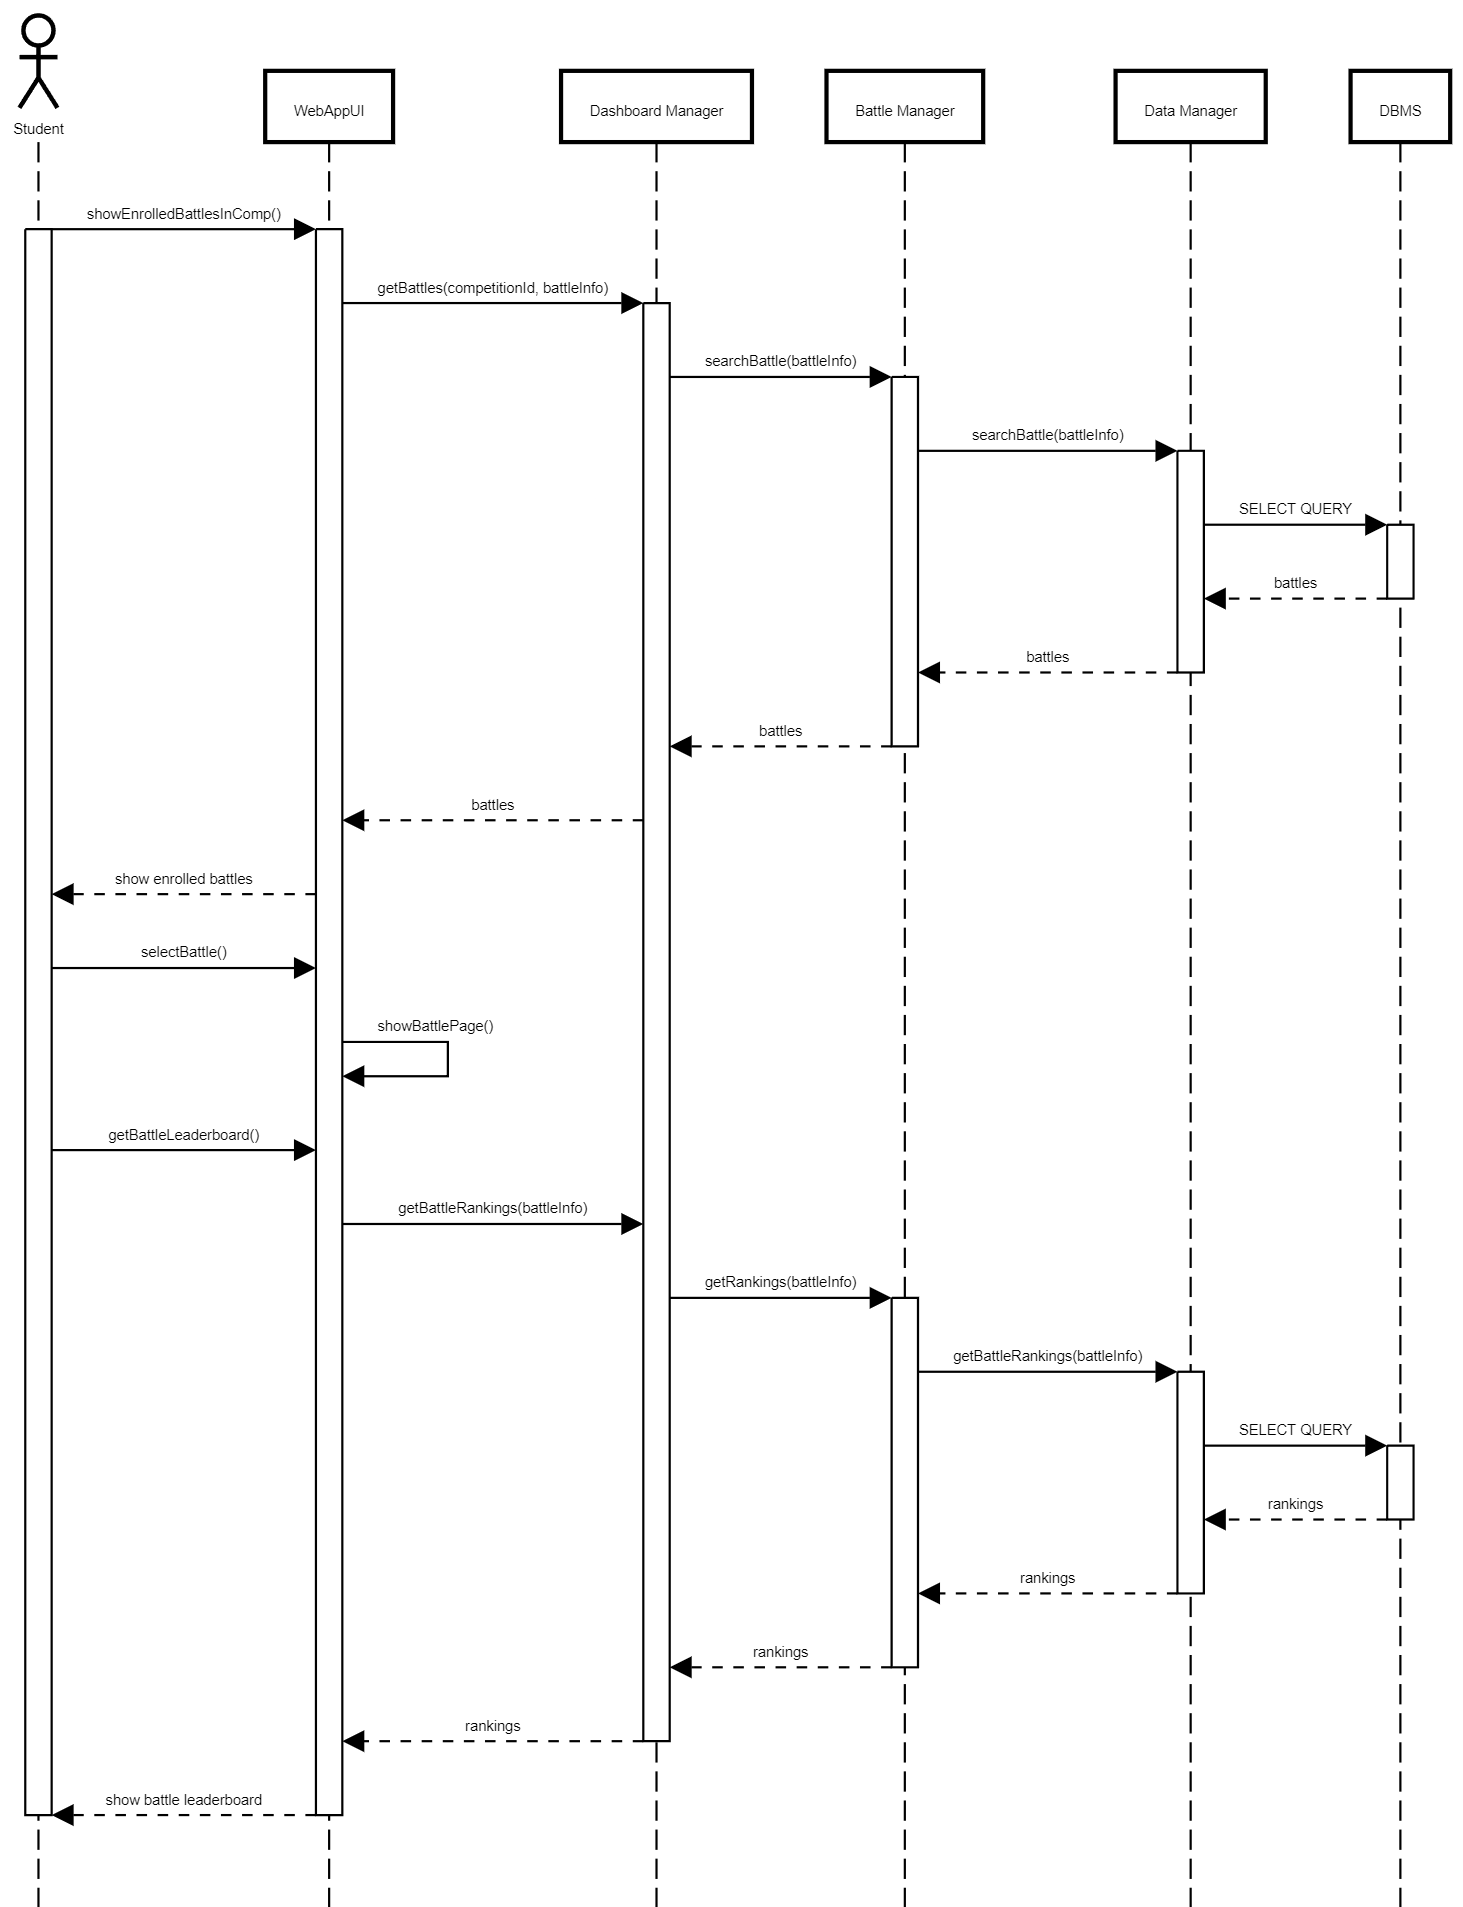
\includegraphics[width=\textwidth,height=0.75\textheight, keepaspectratio]{SequenceDiagrams/10-BattleRankingVisualization.png}
  \caption{Create battle sequence diagram}
  \label{fig:user_visualize_rankings}
\end{figure}

%11
\subsection*{ED Evaluates Code}
An ED can select a T from the list of teams participating to a battle and evaluate its last commit. In particular the ED after selecting the team, he/she can visualize some brief information about the latest commit of the T, from the visualization is possible to navigate to the Github page of the commit. After reviewing the code on Github the ED can return to the CKB page and insert the evaluation of the commit. The process is handled by the \textit{Team Manager} component, which interacts with the \textit{Data Manager} component to insert the evaluation into the DBMS.

\begin{figure}[H]
  \centering
  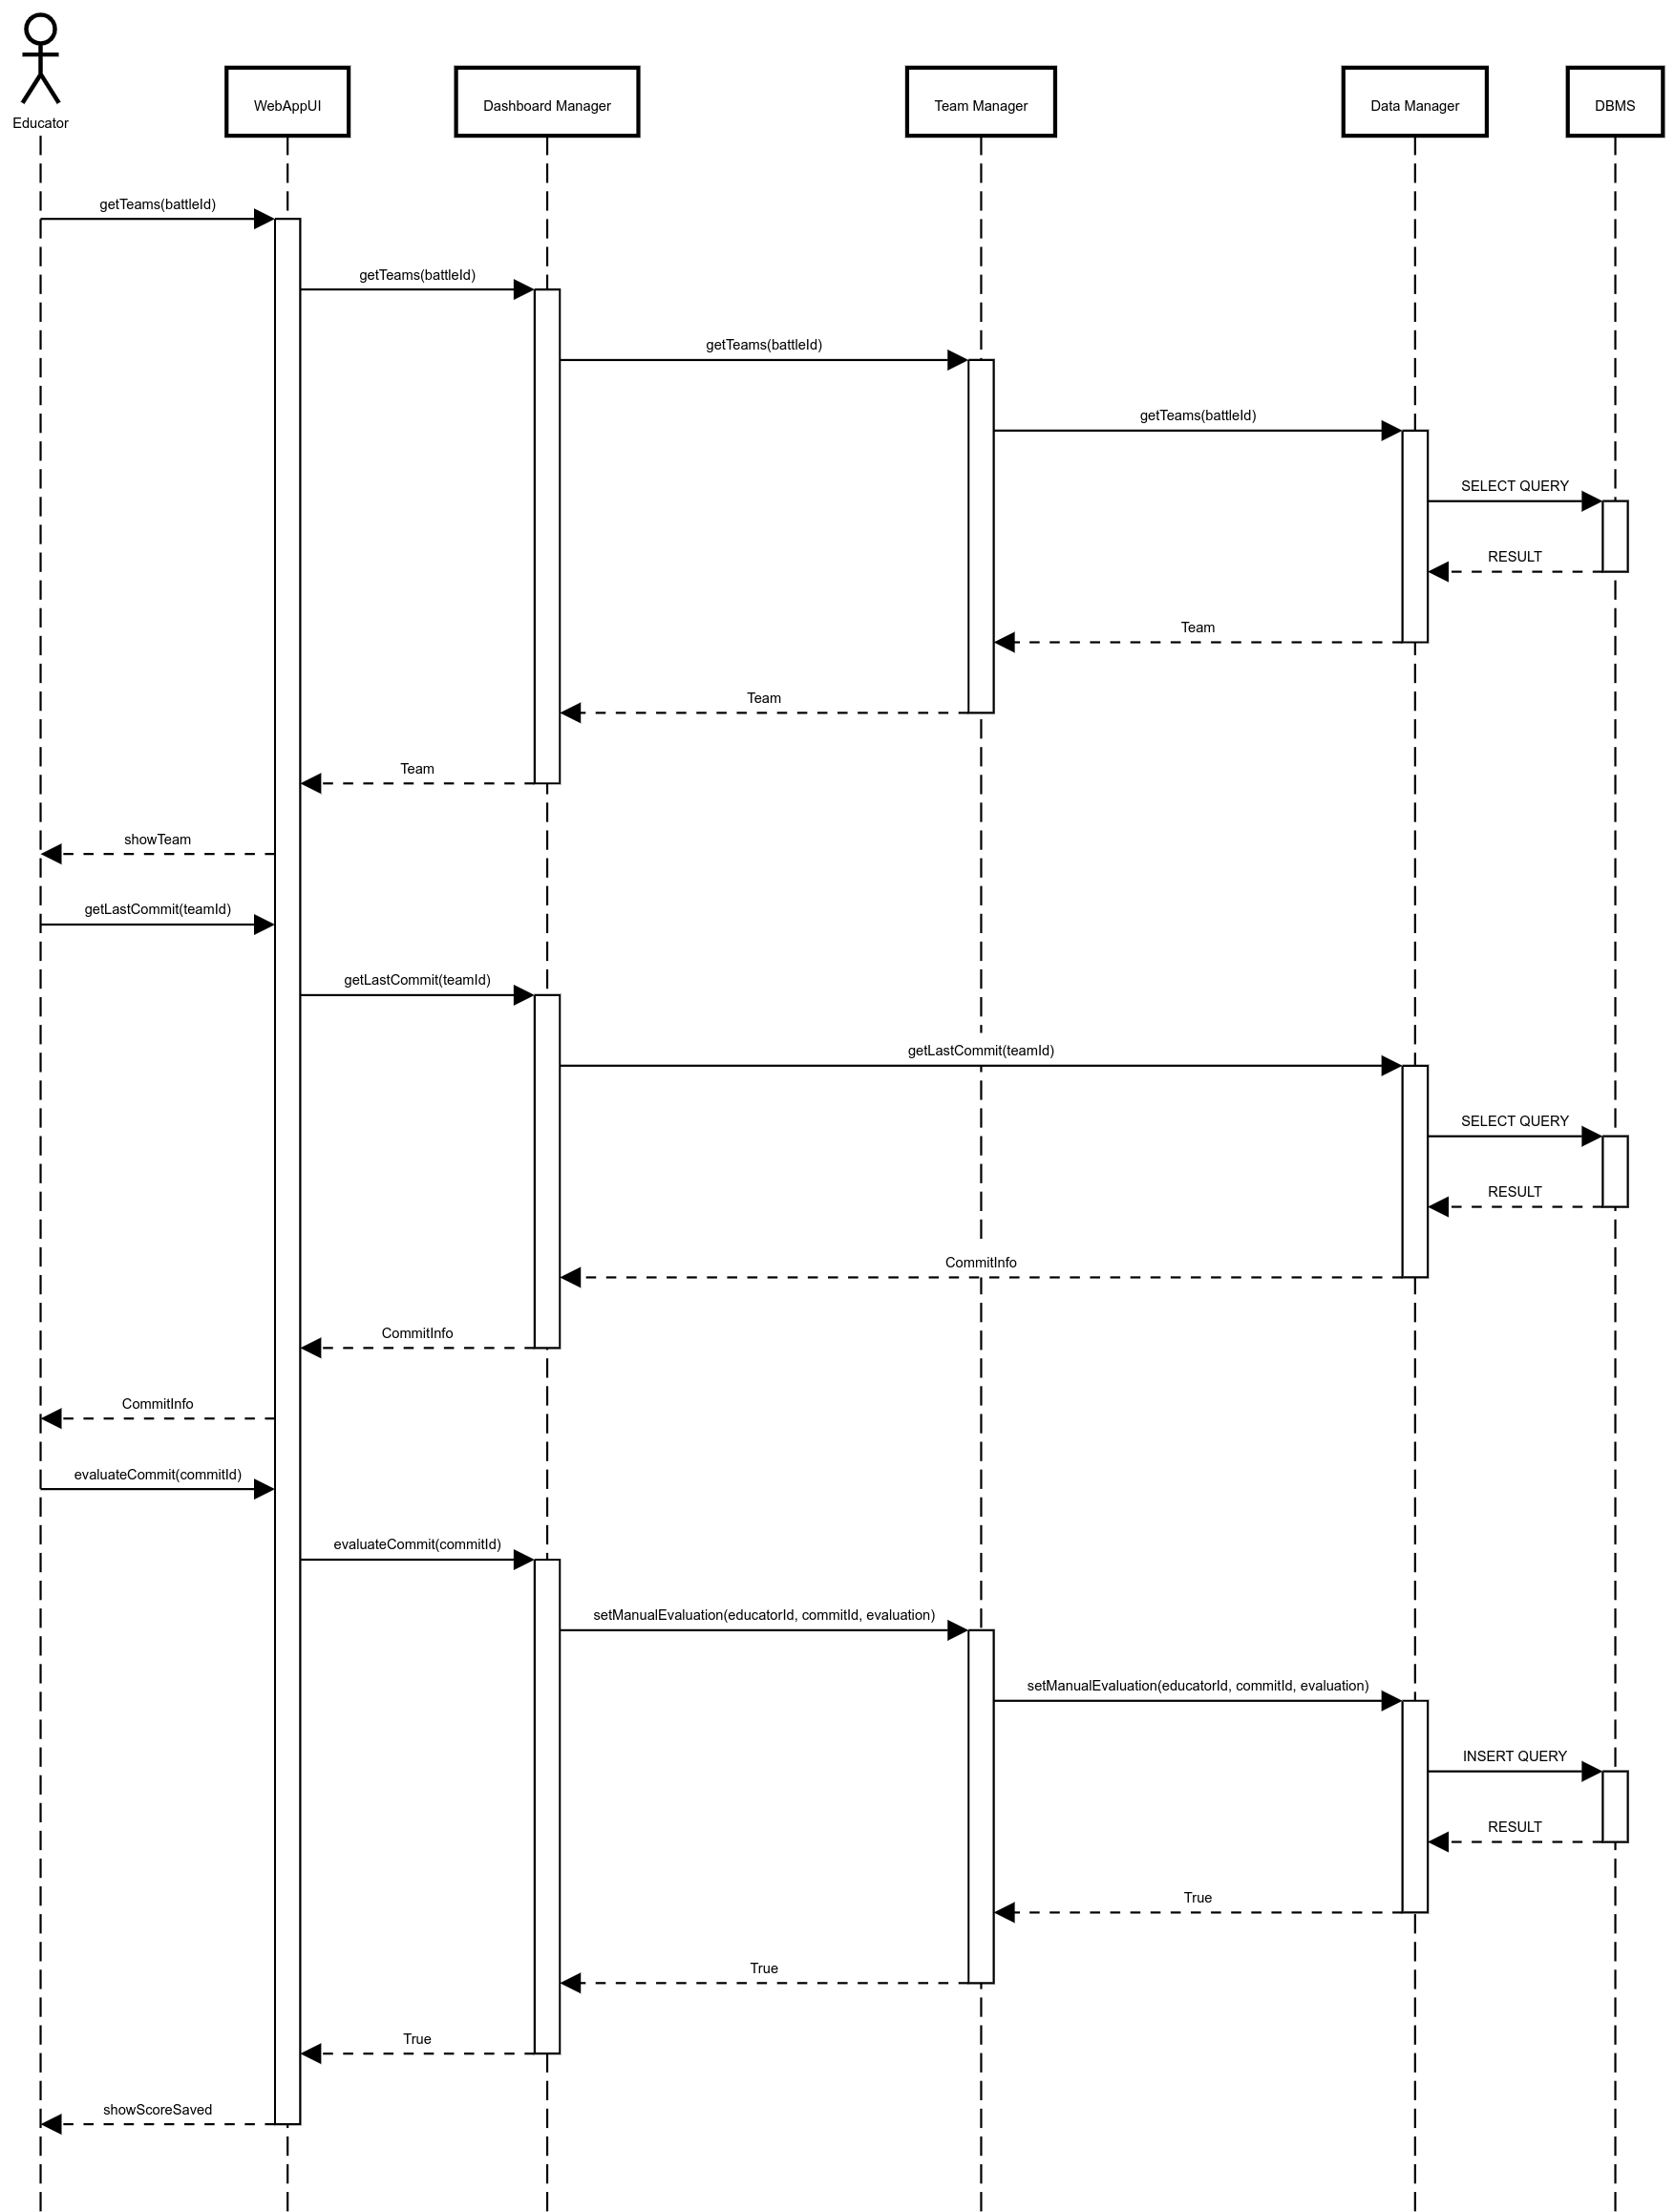
\includegraphics[width=\textwidth,height=0.7\textheight, keepaspectratio]{SequenceDiagrams/11-EdEvaluatesCode.png}
  \caption{ED evaluates code sequence diagram}
  \label{fig:ed_evaluates_code}
\end{figure}

%12
\subsection*{ST Accepts invite}
When a ST clicks on the link in the email received from the system, he/she will be added to the T. The \textit{Team Manager} component will handle the request and will insert the ST into the DBMS using the \textit{Data Manager} component. In case the invitation link is expired, the system will show an error message to the user.

\begin{figure}[H]
  \centering
  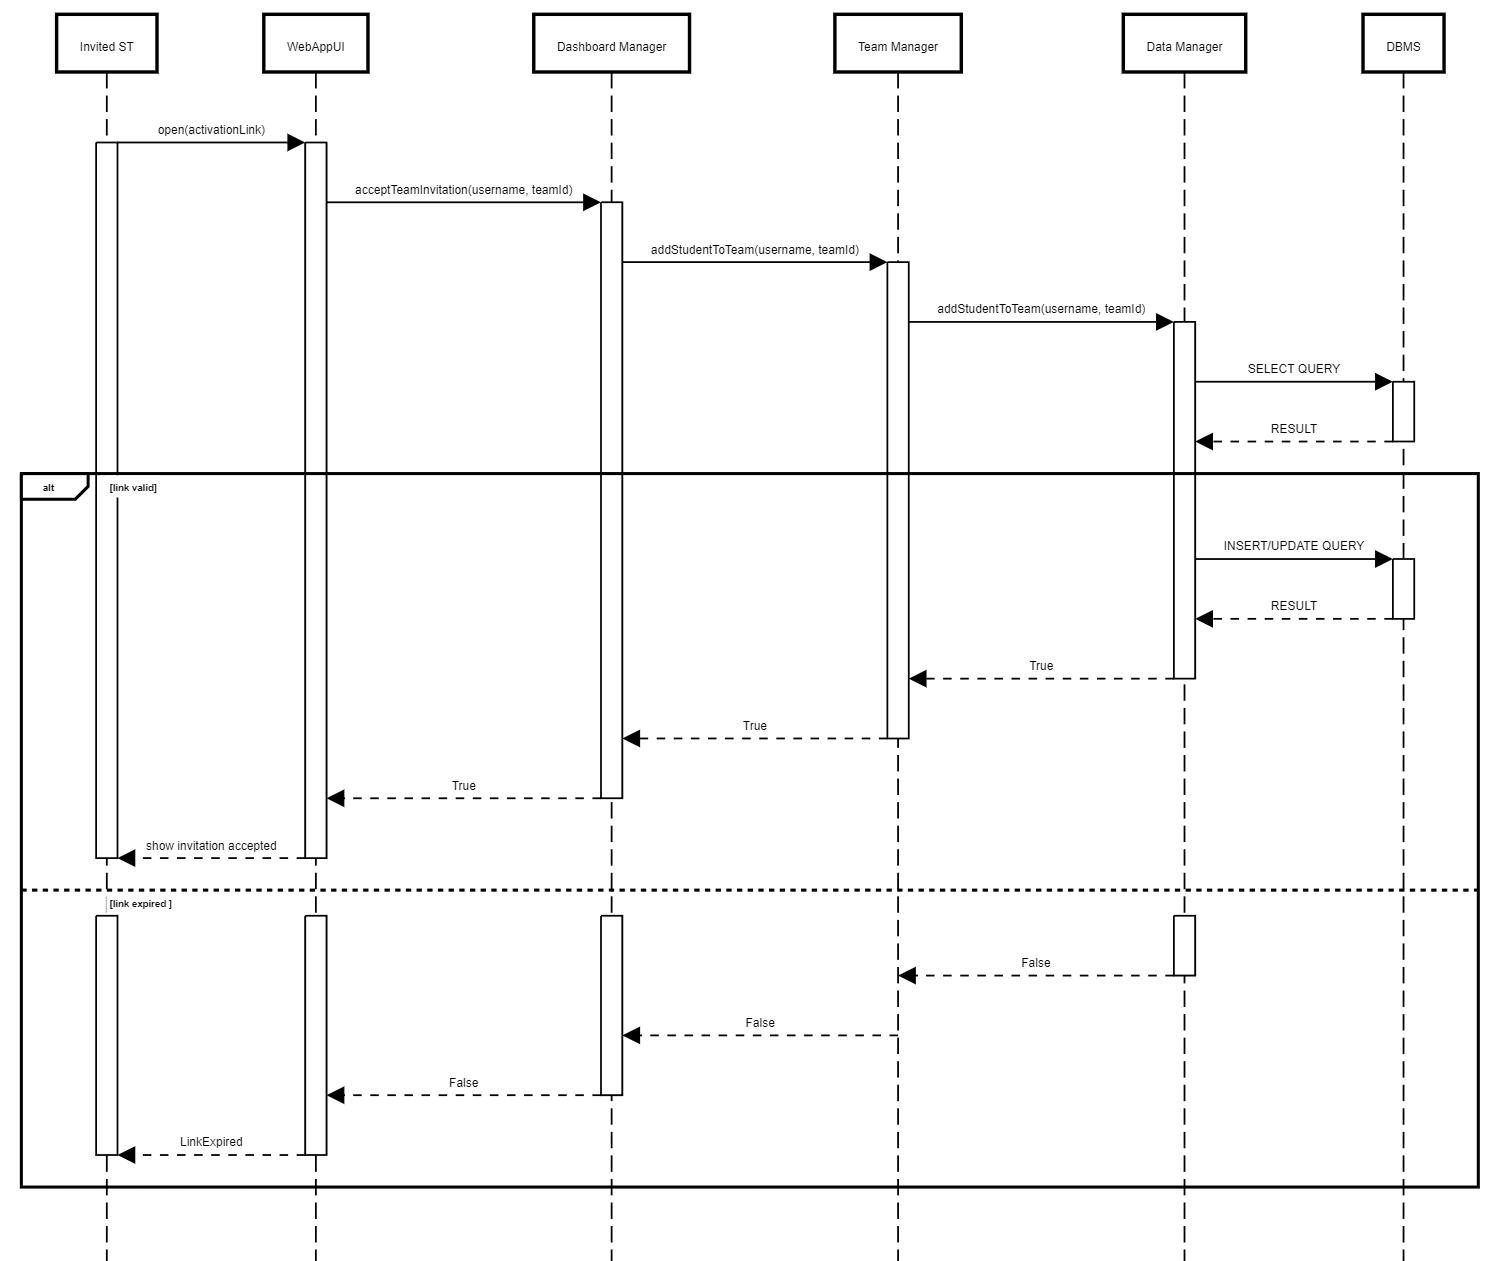
\includegraphics[width=\textwidth,height=\textheight, keepaspectratio]{SequenceDiagrams/12-StAcceptInvite.png}
  \caption{ST accepts invite sequence diagram}
  \label{fig:st_accepts_invite}
\end{figure}

%13
\subsection*{ST Visualizes other ST Profile}
STs can visualize the profile of other STs. The ST can search for a specific ST using its username, the system will show the list of the corresponding STs and the ST can select one of them to visualize its profile. In the profile page the ST can see some information about the ST and the list of the badges that he/she has earned. The \textit{Dashboard Manager} component will handle the request and will retrieve the information from the DBMS using the \textit{Data Manager} component.

\begin{figure}[H]
  \centering
  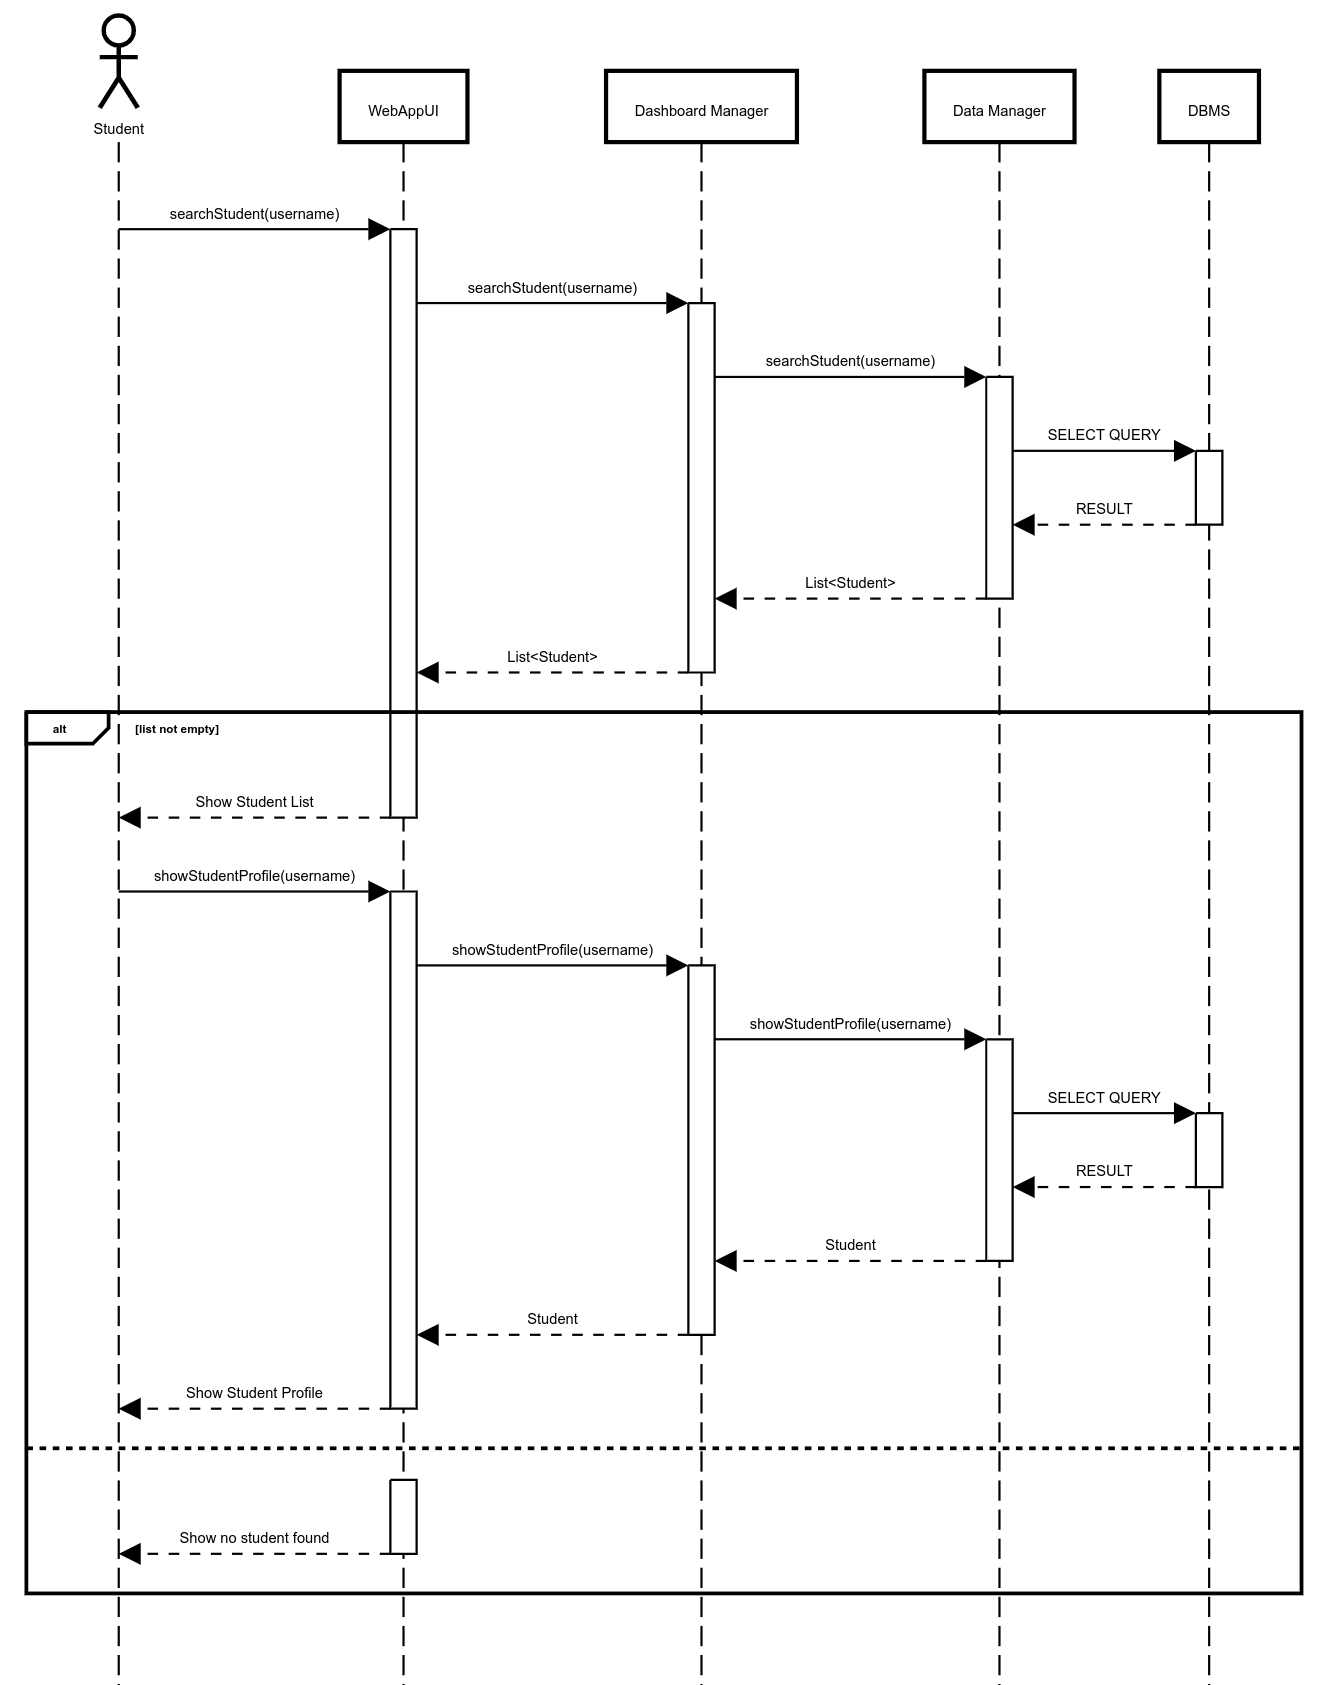
\includegraphics[width=\textwidth,height=\textheight, keepaspectratio]{SequenceDiagrams/13-StudentVisualizeSTprofile.png}
  \caption{ST visualizes other ST profile sequence diagram}
  \label{fig:st_visualizes_other_st_profile}
\end{figure}

\section{Component interfaces}
\label{s:component-interfaces}%


\subsection{Authentication Service}
\subsubsection{AuthInterface}
\begin{itemize}
    \item \texttt{User login(username:String,password:String)}%x
    \item \texttt{bool register(info:UserInfo)} %x
\end{itemize}

\subsection{Data Manager}
\subsubsection{AuthDAOInterface}
\begin{itemize}
    \item \texttt{bool addUser(info: UserInfo)}%x
    \item \texttt{bool checkCredential(username:String,password:String)}%x
    \item \texttt{bool validateNewUser(info:UserInfo)}%x
    \item \texttt{User getUser(username:String)}%x
\end{itemize}

\subsubsection{CompetitionDAOInterface}
\begin{itemize}
    \item \texttt{bool createCompetition(info:CompetitionInfo)}
    \item \texttt{bool addStudentToCompetition(competitionName:String, studentUsername:String)}
    \item \texttt{bool checkEdCanbeInvited(competitionName:String,educatorId:String)}%x
    \item \texttt{Competition getCompetition(name:String)}%x
    \item \texttt{List<Team> getCompRankings(competitionid: String)}
\end{itemize}

\subsubsection{BattleDAOInterface}
\begin{itemize}
    \item \texttt{bool createBattle(competitionName:String, battleInfo:BattleInfo,\\educatorId:String)}%x
    \item \texttt{Set<Battle> searchBattle(battleInfo:BattleInfo)}
    \item \texttt{List<Battle> searchBattleInCompetition(competitionId:String)}%x
    \item \texttt{Battle showBattle(battleName:String)}
    \item \texttt{List<Team> getBattleRankings(battleid: String)}
    \item \texttt{bool insertBattleConfiguration(battleConfiguration:BattleConfiguration,\\battleName:String,educatorId:String)}%x
\end{itemize}

\subsubsection{UserDAOInterface}
\begin{itemize}
    \item \texttt{Team createTeam(battleId:String, teamInfo:TeamInfo)}%x
    \item \texttt{bool removeTeam(teamId:String)}
    \item \texttt{bool addStudentToTeam(username:String,teamId:String)}%x
    \item \texttt{bool setManualEvaluation(educatorId:String,commitId:String,evaluation: Evaluation)}%x
    \item \texttt{Team getTeams(battleid: String)}%x
\end{itemize}

\subsubsection{BadgeDAOInterface}
\begin{itemize}
    \item \texttt{Set<User> retrieveUsersFromCompetition(competitionName:String)}
    \item \texttt{BadgeRule getBadgeRule(badge: Badge)}
    \item \texttt{bool removeBadge(badge:Badge)}
    \item \texttt{bool assignBadge(username:String, badge:Badge)}
    \item \texttt{bool createBadge(educatorId:String,competitionId:String, badgeInfo:BadgeInfo)}%x
\end{itemize}

\subsubsection{NotificationDAOInterface}
\begin{itemize}
    \item \texttt{Set<Student> retrieveStudentsFromTeam(teamId:String)}
    \item \texttt{Set<User> retrieveUsersFromCompetition(competitionId:String)}
    \item \texttt{Set<Student> retrieveStudentsFromCompetition(competitionId:String)}%x
    \item \texttt{Set<Educator> retrieveEducatorsFromCompetition(competitionId:String)}
    \item \texttt{Set<User> retrieveUsersFromBattle(battleId:String)}
    \item \texttt{Set<Student> retrieveStudentsFromBattle(battleId:String)}
    \item \texttt{Set<Educator> retrieveEducatorsFromBattle(battleId:String)}
    \item \texttt{Educator retrieveEducatorInfo(educatorId:String)}%x
\end{itemize}

\subsubsection{PointsAPI}
\begin{itemize}
    \item \texttt{bool addEvaluationToTeam(teamId:string, evaluation:Evaluation)}
\end{itemize}

\subsubsection{DashboardDAOInterface}
\begin{itemize}
    \item \texttt{List<Student> searchStudent(studentName:String)}%x
    \item \texttt{Student showStudentProfile(username:String)}%x
    \item \texttt{CommitInfo getLastCommit(teamId: String)}%x
\end{itemize}

\subsection{Dashboard Manager}
\subsubsection{DashboardInterface}
\begin{itemize}
    \item \texttt{DashboardInfo getDashboardInfo(User)}%x
    \item \texttt{createCompetition(competitionInfo:CompetitionInfo)}%x
    \item \texttt{bool createBattle(battleInfo:BattleInfo,competitionName:String,\\educatorId:String)}%x
    \item \texttt{bool joinCompetition(competitionName:String, studentUsername:String)}%x
    \item \texttt{CompetitionInfo showCompetition(name:String)}%x
    \item \texttt{List<Battle> getBattles(competitionid: String)}%x
    %@toCheck
    \item \texttt{Battle getBattle(competitionid: String, battleId: String)}
    %\item \texttt{bool insertSATConfiguration(satConfiguration:SatConfiguration,\\battleName:String,educatorId:String)}%x
    \item \texttt{bool insertBattleConfiguration(battleConfiguration:BattleConfiguration, \\battleName:String,educatorId:String)}%x
    \item \texttt{bool inviteStudentToTeam(username: String, teamid: String)}%x
    \item \texttt{List<Team> getTeams(battleid: String)}%x
    \item \texttt{bool joinTeam(username: String,teamid: String)}%x
    \item \texttt{List<Team> getCompRankings(competitionid: String)}
    \item \texttt{List<Team> getBattleRankings(battleInfo: BattleInfo)}
    \item \texttt{List<Student> searchStudent(studentName:String)}%x
    \item \texttt{Student showStudentProfile(username:String)}%x
    \item \texttt{CompetitionSetting showCompetitionSettings(educatorId:String,\\competitionId:String)}%x
    \item \texttt{BadgeCreation showBadgeCreation(educatorId:String,\\competitionId:String)}%x
    \item \texttt{InviteEdPanel showInviteEd(educatorId:String,competitionId:String)}%x
    \item \texttt{bool inviteED(educatorId:String,competitionId:String,invitedEducatorId:String)}%x
    \item \texttt{bool createBadge(educatorId:String,competitionName:String, badgeInfo: BadgeInfo)}%x
    \item \texttt{CommitInfo getLastCommit(teamId: String)}%x
    \item \texttt{bool acceptInvitation(educatorId:String,competitionId:String)}%x
    \item \texttt{bool acceptTeamInvitation(username:String,teamId:String)}%x
    \item \texttt{Team createTeam(battleid: String, username: String)}%x
    \item \texttt{bool evaluateCommit(commitId: String)}%x
\end{itemize}

\subsection{Competition Manager}
\subsubsection{CompetitionInterface}
\begin{itemize}
    \item \texttt{Competition createCompetition(info:CompetitionInfo)}%x
    \item \texttt{Set<Competition> searchCompetition(info:CompetitionInfo)}
    \item \texttt{bool deleteCompetition(name:String)}
    \item \texttt{Competition getCompetition(name:String)}%x
    \item \texttt{bool addManager(competitionName:String,username:String)}%x
    \item \texttt{bool removeManager(competitionName:String,username:String)}
    \item \texttt{bool endCompetition(competitionName:String)}
    \item \texttt{bool joinCompetition(competitionName:String, studentUsername:String)}%x
    \item \texttt{bool createBadge(educatorId:String,competitionName:String, badgeInfo: BadgeInfo)}%x
    \item \texttt{bool removeBadge(badgeId:String)}
    \item \texttt{List<Team> getRankings(competitionid: String)}
    \item \texttt{bool acceptInvitation(educatorId:String,competitionId:String)}%x
    \item \texttt{bool inviteED(educatorId:String,competitionId:String,invitedEducatorId:String)}%x
\end{itemize}

\subsection{Badge Manager}
\subsubsection{BadgeInterface}
\begin{itemize}
    \item \texttt{bool createBadge(competitionName:String, badgeInfo: BadgeInfo)}%x
    \item \texttt{bool assignBadges(competitionName:String)}
    \item \texttt{bool removeBadge(badgeId:String)}
\end{itemize}

\subsection{BattleManager}
\subsubsection{BattleInterface}
\begin{itemize}
    \item \texttt{bool createBattle(competitionName:String, battleInfo:BattleInfo,\\ educatorId:String)}
    \item \texttt{Team createTeam(battleId:String, teamInfo:TeamInfo)}%x
    \item \texttt{bool removeTeam(teamId:String)}
    \item \texttt{List<Battle> searchBattle(battleInfo:BattleInfo)}
    \item \texttt{List<Battle> searchBattleInCompetition(competitionId:String)}%x
    \item \texttt{Battle showBattle(battleName:String)}
    \item \texttt{bool deleteBattle(battleName:String)}
    %\item \texttt{insertSATConfiguration(satConfiguration,battleName,educatorId)}
    \item \texttt{bool insertBattleConfiguration(battleConfiguration:BattleConfiguration, \\battleName:String,educatorId:String)}%x
    \item \texttt{List<Team> getRankings(battleid: String)}
\end{itemize}

\subsection{Team Manager}
\subsubsection{TeamHandlerInterface}
\begin{itemize}
    \item \texttt{Team createTeam(battleId:String, teamInfo:TeamInfo)}
    \item \texttt{bool removeTeam(teamId:String)}
    \item \texttt{Team getTeams(battleid: String)}%x
\end{itemize}

\subsubsection{TeamInterface}
\begin{itemize}
    \item \texttt{bool addStudentToTeam(username:String,teamId:String)}%x
    \item \texttt{bool inviteStudentToTeam(username:String,teamId:String)}%x
    \item \texttt{bool setManualEvaluation(educatorId:String,commitId:String,evaluation: Evaluation)}%x
\end{itemize}


\subsection{Notification Service}
\subsubsection{InviteInterface}
\begin{itemize}
    \item \texttt{bool inviteStudentToTeam(username:String,teamId:String)}%x
\end{itemize}

\subsubsection{NotifyBattleInterface}
\begin{itemize}
    \item \texttt{bool notifyBattleCreation(battleId:String, competitionId:String)}%x
    \item \texttt{bool notifyStartedBattle(battleId:String,username:String)}
    \item \texttt{bool notifyEndBattle(battleId:String,username:String)}
    \item \texttt{bool notifyManageBattle(battleId:String,username:String)}
\end{itemize}

\subsubsection{NotifyCompInterface}
\begin{itemize}
    \item \texttt{bool notifyNewCompetion(competitionId:String,username:String)}
    \item \texttt{bool notifyNewBattle(competitionId:String, battleId:String,username:String)}
    \item \texttt{bool notifyEdInvitation(competitionId:String,invitedEd:String)}%x
    \item \texttt{bool notifyManageCompetition(competitionId:String,username:String)}
\end{itemize}

\subsubsection{NotifyAuthInterface}
\begin{itemize}
    \item \texttt{bool NotifyUserRegistration(User)}%x
\end{itemize}

\subsection{Evaluator Controller}
\subsubsection{EvaluationAPI}
\begin{itemize}
    \item \texttt{bool pullCode(authorId:String, commitId:String)}
\end{itemize}

\subsection{Code Evaluator}
\subsubsection{EvaluatorInterface}
\begin{itemize}
    \item \texttt{bool evaluateCode(authorId:String, commitId:String)}
    \item \texttt{void setConf(conf: EvalConfig)}
\end{itemize}

\subsection{Static Analyzer}
\subsubsection{AnalyzerInterface}
\begin{itemize}
    \item \texttt{bool evaluateCode(authorId:String, commitId:String, params:String)}
    \item \texttt{void setConf(conf: StatConfig)}
\end{itemize}

\subsection{Point Manager}
\subsubsection{EvaluationPointsInterface}
\begin{itemize}
    \item \texttt{bool assignPoint(authorId:String, evalResults: EvalResults)}
\end{itemize}

\subsubsection{StaticPointsInterface}
\begin{itemize}
    \item \texttt{bool assignPoint(authorId:String, statResults: StatResults)}
\end{itemize}

\subsubsection{ScoreInterface}
\begin{itemize}
    \item \texttt{void setEvalScoreFunction(conf: EvalScoreFunction)}
    \item \texttt{void setStatAnalysisScoreFunction(conf: StatScoreFunction)}
\end{itemize}

\newpage

\section{Selected architectural styles and patterns}
\label{s:selected-architectural-styles-and-patterns}%

\subsection{Client-Server}
Since the CKB is a platform offered through the web, the client-server architecture is the most suitable for this kind of application. In particular we are using a 3-tier architecture, where the client is the web browser, the server is the application server and the database is the data server. This architecture is the most suitable for our application because it allows us to separate the presentation layer from the business logic and the data layer. Moreover, this separation allows us to have a more maintainable and scalable application.

\subsection{REST}
The communication between the client and the server is based on the REST architectural style. The REST architectural style is stateless, this means that the server does not need to store any information about the client session, this allows us to have a more scalable application. Moreover, in combination with the HTTP protocol, it allows us to provide a uniform interface to the client, which is based on the HTTP methods (GET, POST, PUT, DELETE).

\subsection{MVC}
The MVC pattern is used to separate the presentation layer from the business logic. In particular, the \textit{Model} is represented by the \textit{Data Manager} component, the \textit{View} is represented by the \textit{WebAppUI} component and the \textit{Controller} is represented by all the other \textit{Managers} component. This pattern allows us to have a more maintainable application, because the changes in one layer do not affect the other layers.


\section{Other design decisions}
\label{s:other-design-decisions}%

\subsection{SandBox}
To protect the application from malicious code, we decided to use a sandbox. In particular, the code evaluator and the static analyzer will be executed in a sandbox. This allows us to have a more secure application, because the code will be executed in a controlled environment.


\subsection{Database}
We decided to use a relational database to store the data of the application given its structure. In particular, we decided to use PostgreSQL, because it is an open source database and it is one of the most used relational database. Moreover, it is ACID compliant, this means that it guarantees the atomicity, consistency, isolation and durability of the transactions.
%-------------------------------------------------------------------------
%	User interface design
%-------------------------------------------------------------------------
\chapter{User interface design}
\label{c:user_interface_design}%
%
In this section we will describe the user interface design of the system. We will provide a mockup of the main pages of the system and a description of the main functionalities.

The user interface of the system is designed to be simple and intuitive. As the system is intended to be used with a desktop browser, the interfaces presented here are based on a desktop browser, but the interface is thought to be responsive and consequently usable also on mobile devices.

\section*{Common Interfaces}
\label{s:common_interface}%
Some pages of the platform are common, or very similar, for both ST and ED, so in this section we will show only once the mockup of the pages and we will describe the functionalities of the pages for both ST and ED.

\subsubsection*{Login Page}
\label{ss:login}%

\begin{figure}[H]
  \centering
  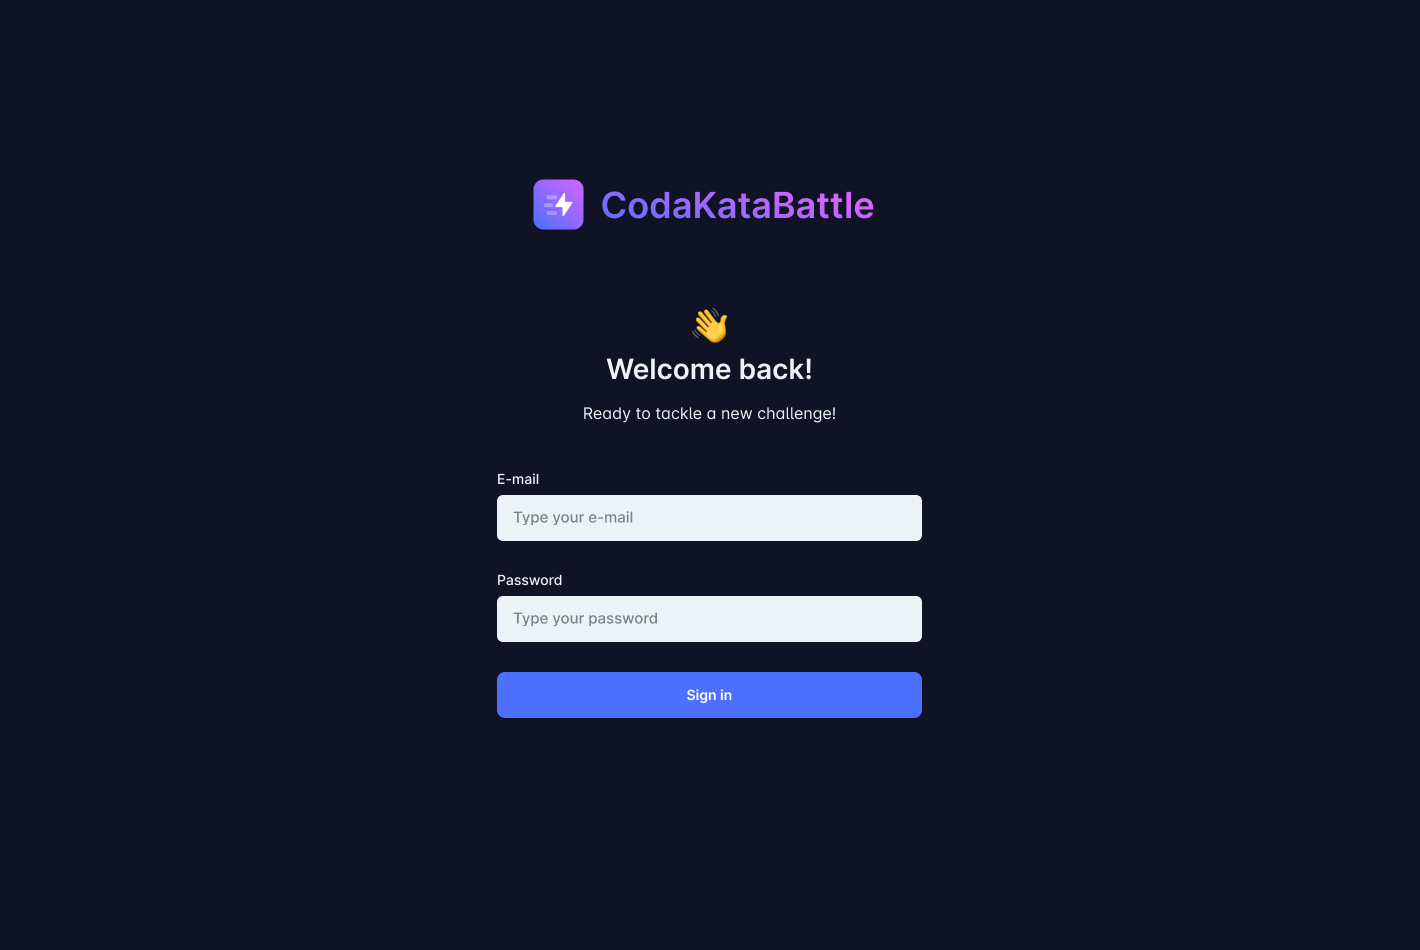
\includegraphics[width=\textwidth]{User Interface/Login.png}
  \caption{CKB login page}
  \label{fig:login}
\end{figure}

\newpage

\subsubsection*{Registration Page}
\label{ss:registration}%
Here for simplicity we show only the registration page for a ST, but the registration page for a ED is equal to this one with the only difference that the ED is required to insert also information about the institution he/she works for.

\begin{figure}[H]
  \centering
  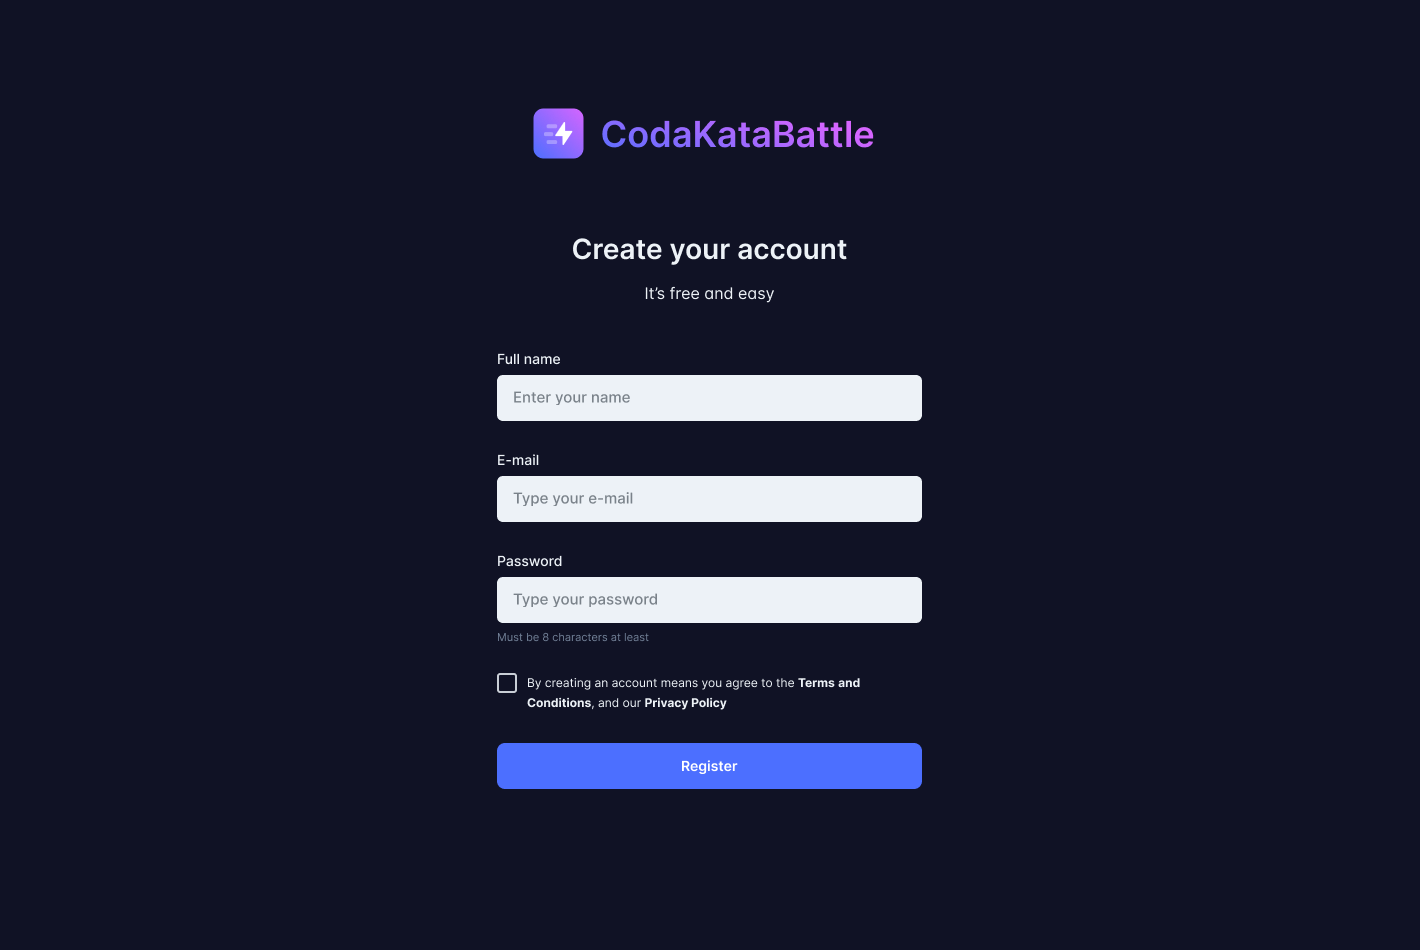
\includegraphics[width=\textwidth]{User Interface/Register.png}
  \caption{CKB registration page}
  \label{fig:registration}
\end{figure}

\newpage

\subsubsection*{Home Page}
\label{ss:home_page}%
This is a mockup of the homepage of a ST. ED would see a very similar home page with statistics about the competition and battle created.

\begin{figure}[H]
  \centering
  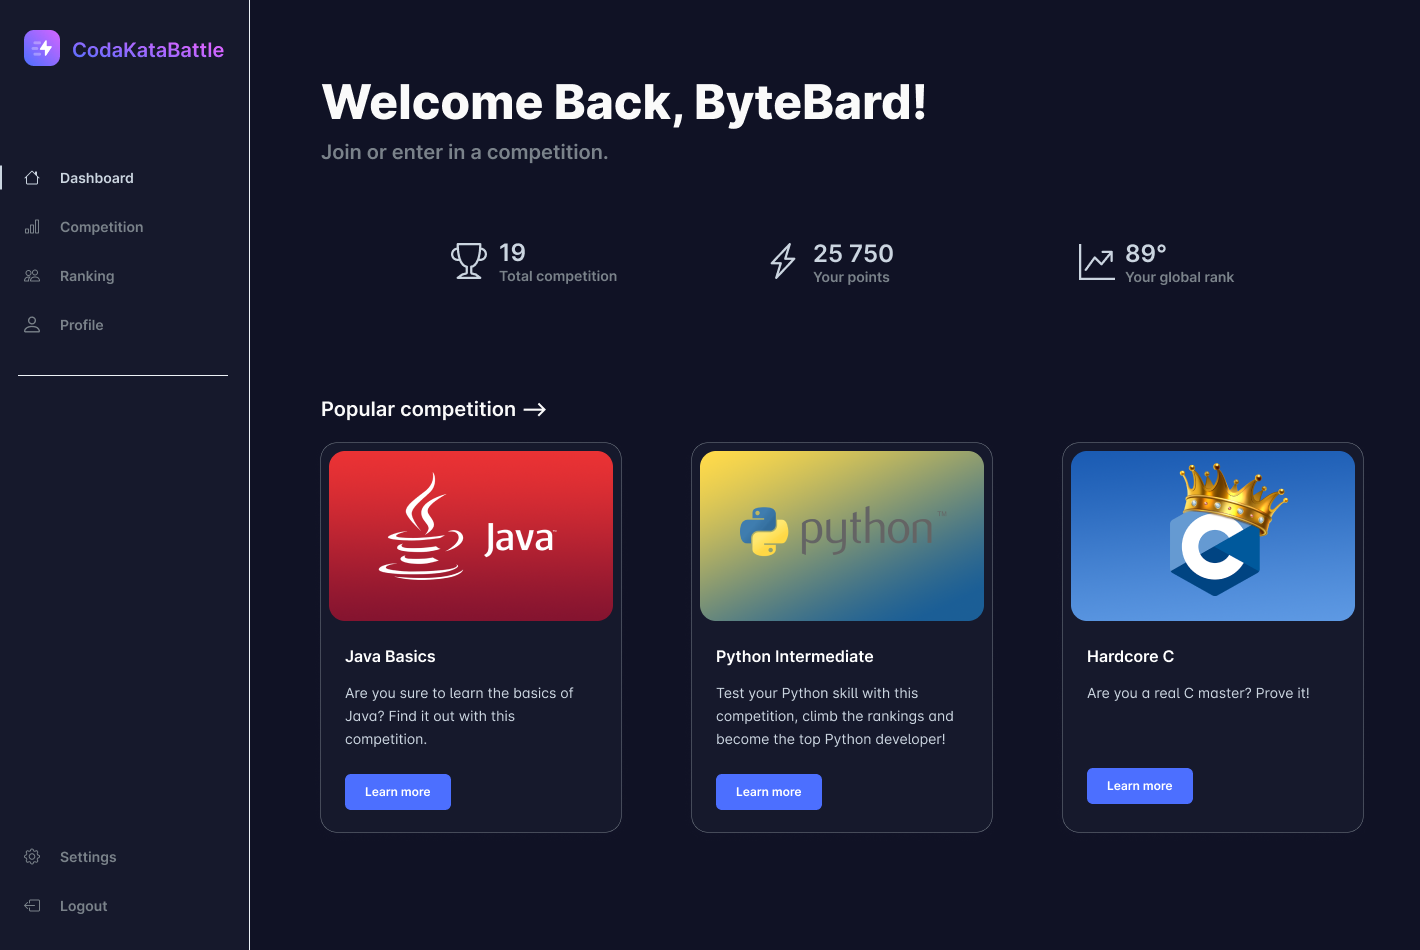
\includegraphics[width=\textwidth]{User Interface/Homepage Student.png}
  \caption{CKB student home page}
  \label{fig:homepage}
\end{figure}

\newpage

\subsubsection*{Competition Page}
\label{ss:competition_page}%
In this page the ST can see the list of all the competitions he/her is currently enrolled in. The ED can see the list of all the competitions he/her has created.

\begin{figure}[H]
  \centering
  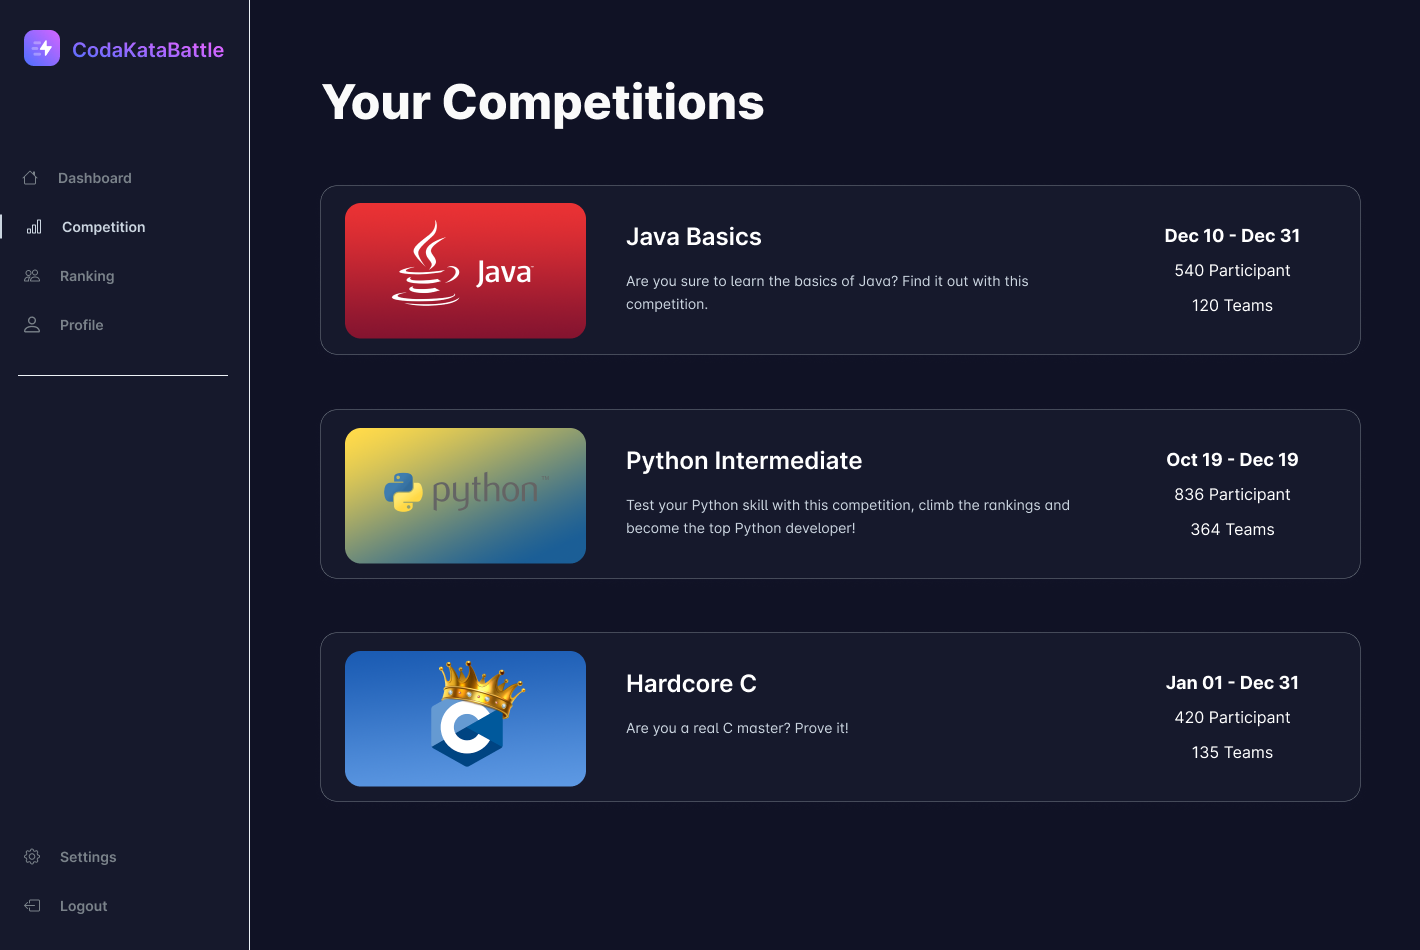
\includegraphics[width=\textwidth]{User Interface/Competition.png}
  \caption{CKB competition page}
  \label{fig:competition}
\end{figure}

\newpage

\subsubsection*{Ranking Page}
\label{ss:ranking_page}%
This is a the mockup of all the rankings present in the system. In particular, this is equal for the global ranking, competition raning and battle ranking pages. Both the ST and the ED are presented with the same interface and functionalities when consulting the ranking pages.

\begin{figure}[H]
  \centering
  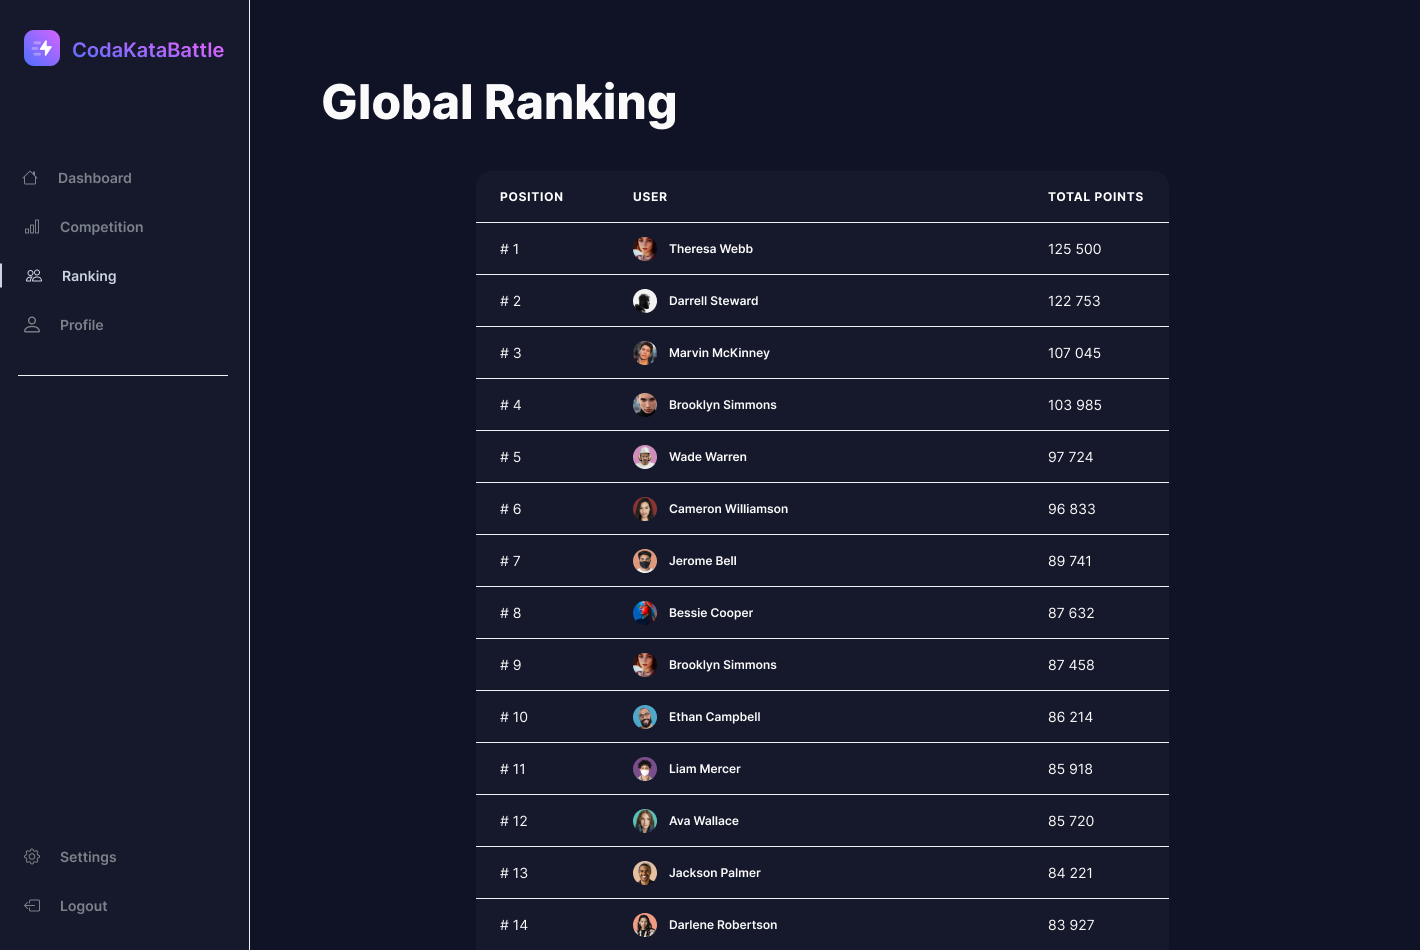
\includegraphics[width=\textwidth]{User Interface/Ranking.png}
  \caption{CKB global ranking page}
  \label{fig:ranking}
\end{figure}

\newpage

\subsubsection*{ST Profile Page}
\label{ss:ST_profile_page}%
Also this page is equal for both ST and ED. In particular in this page it is possible to see all the badges earned by the ST, other than the information about the competition he/her has partecipated in and their statistics.

\begin{figure}[H]
  \centering
  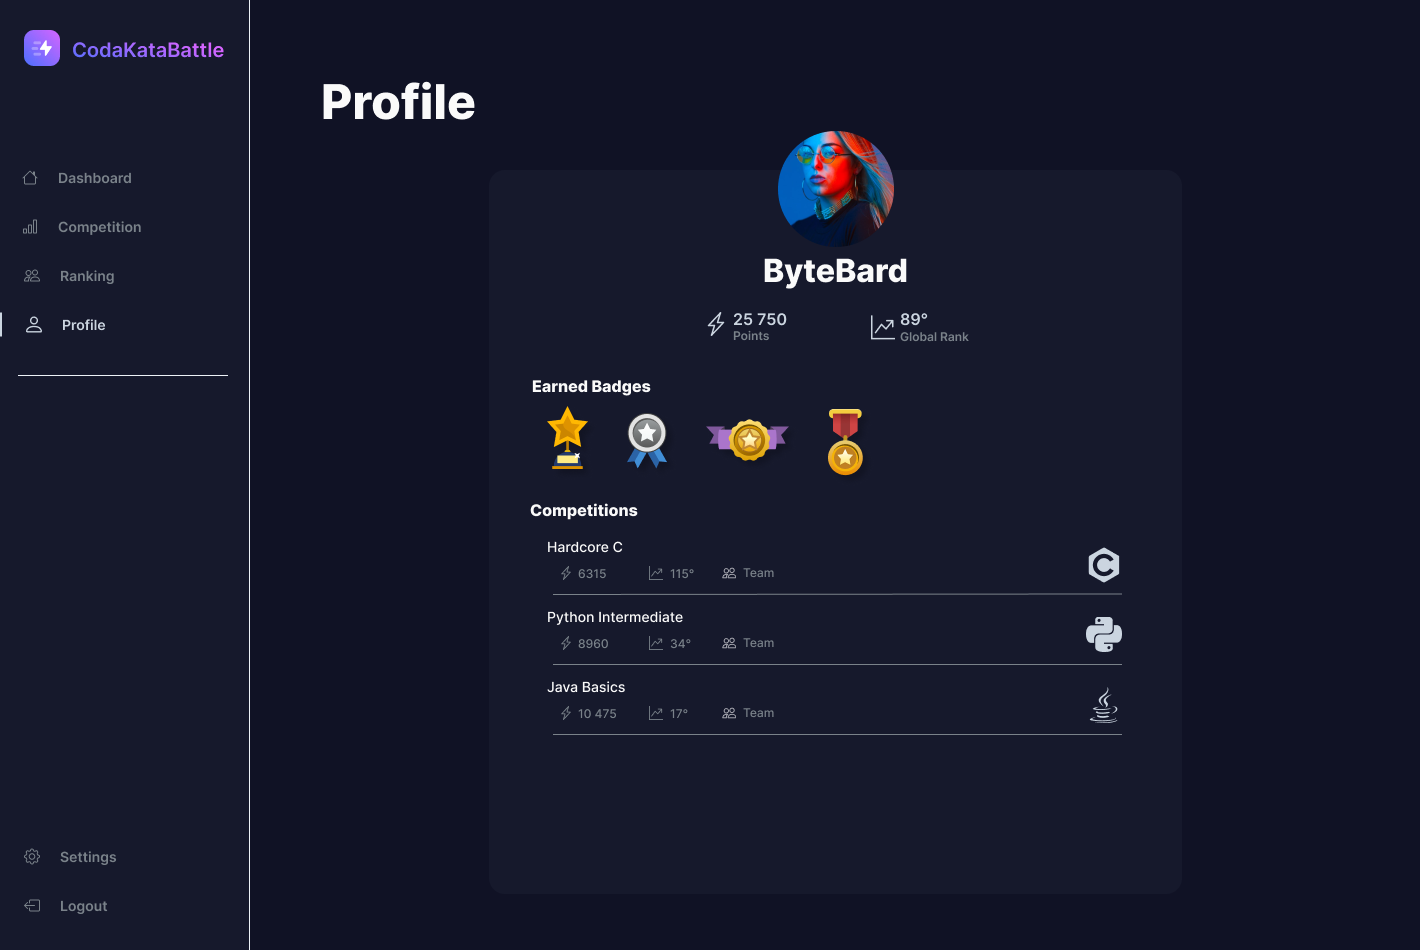
\includegraphics[width=\textwidth]{User Interface/Profile Student.png}
  \caption{CKB ST profile page}
  \label{fig:ST_profile}
\end{figure}

\newpage

\section*{ST Interfaces}
\label{s:ST_interface}%

Now are presented the interfaces that are specific for the ST, in particular are shown the pages relative to the join of a battle by the ST.

\subsubsection*{Join Battle Pages}
\label{ss:join_battle_pages}%
To create a more pleasant experience for the ST, the join battle pages are divided in different steps. In particular, the first step is to choose to join with a T or as a single ST. In the second step, if the ST has decided to join as a T he/her has to choose if he/her wants to create a new T or join an existing one. In case the ST has decided to create a new T is presented with the relative page, otherwise he/her is presented with the page to join an existing public T.

\begin{figure}[H]
  \centering
  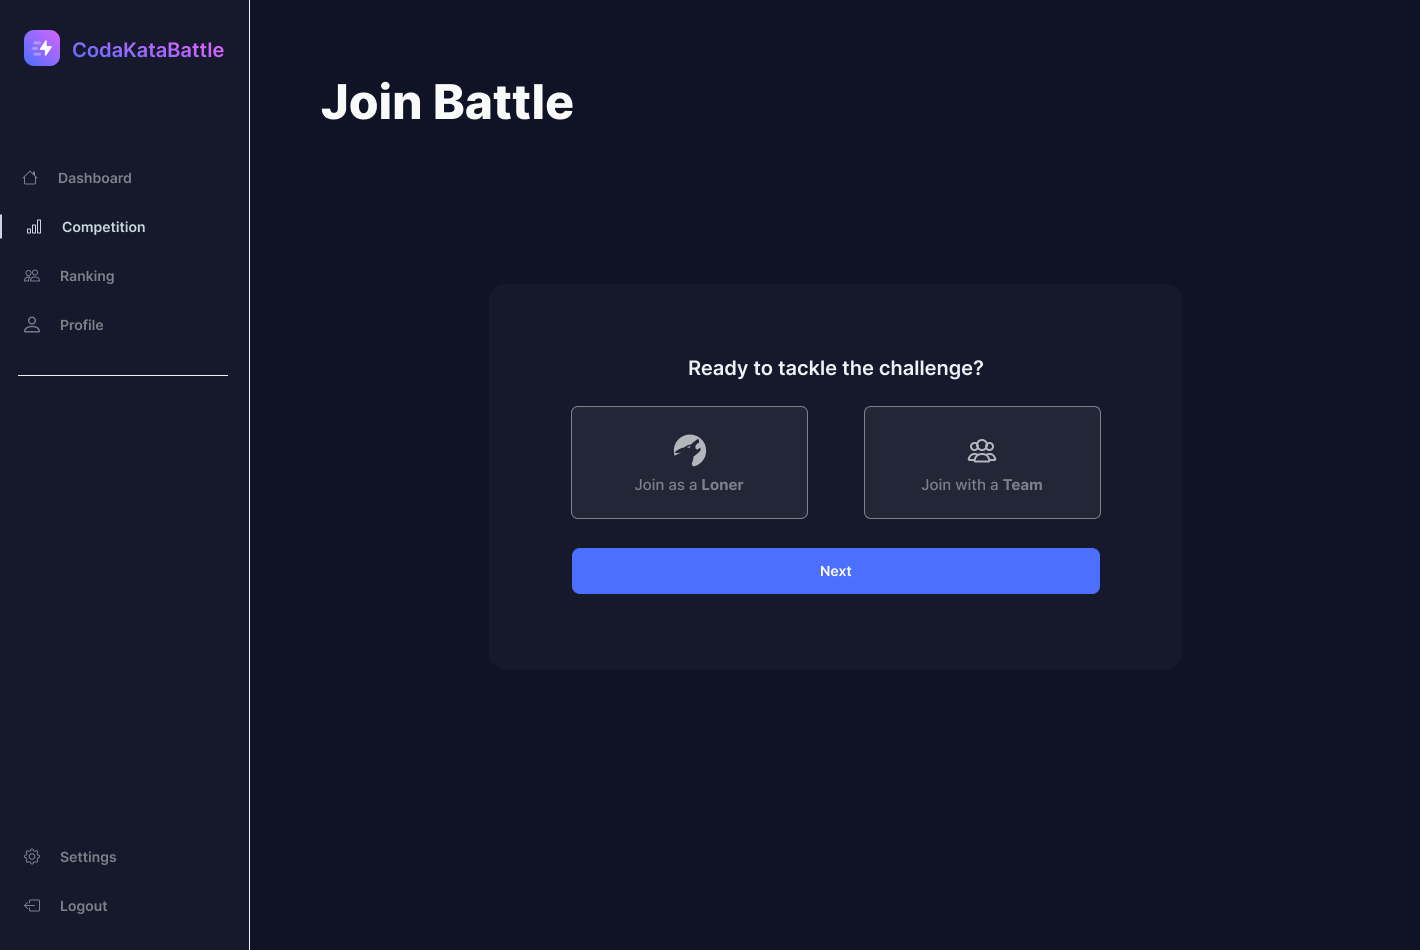
\includegraphics[width=\textwidth]{User Interface/Join Battle Student - 1.png}
  \caption{Join battle page - step 1}
  \label{fig:join_battle1}
\end{figure}

\begin{figure}[H]
  \centering
  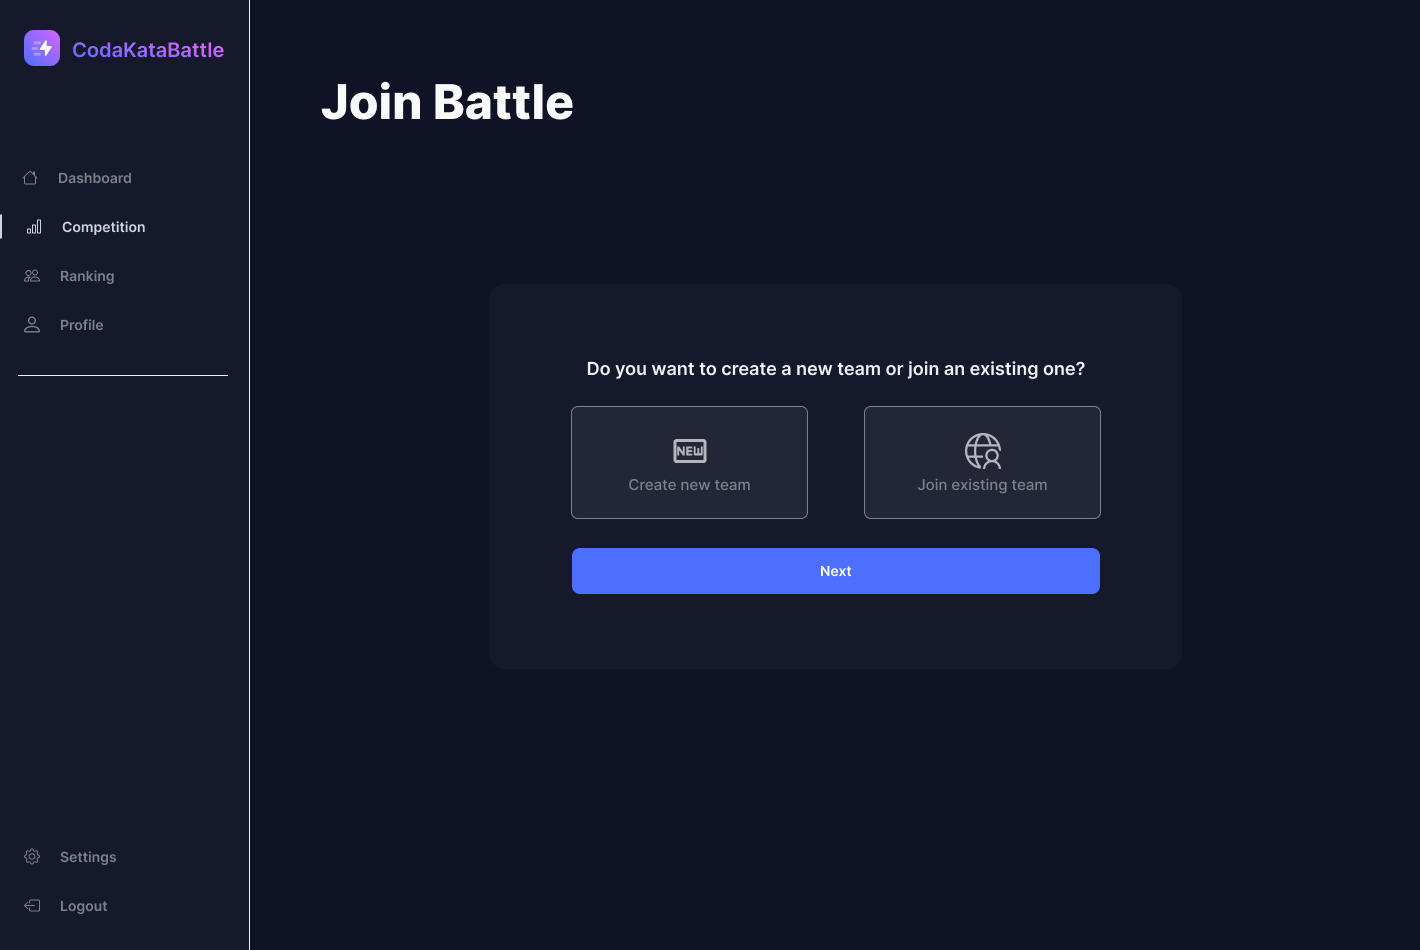
\includegraphics[width=0.95\textwidth]{User Interface/Join Battle Student - 2.png}
  \caption{Join battle page - step 2}
  \label{fig:join_battle2}
\end{figure}

\begin{figure}[H]
  \centering
  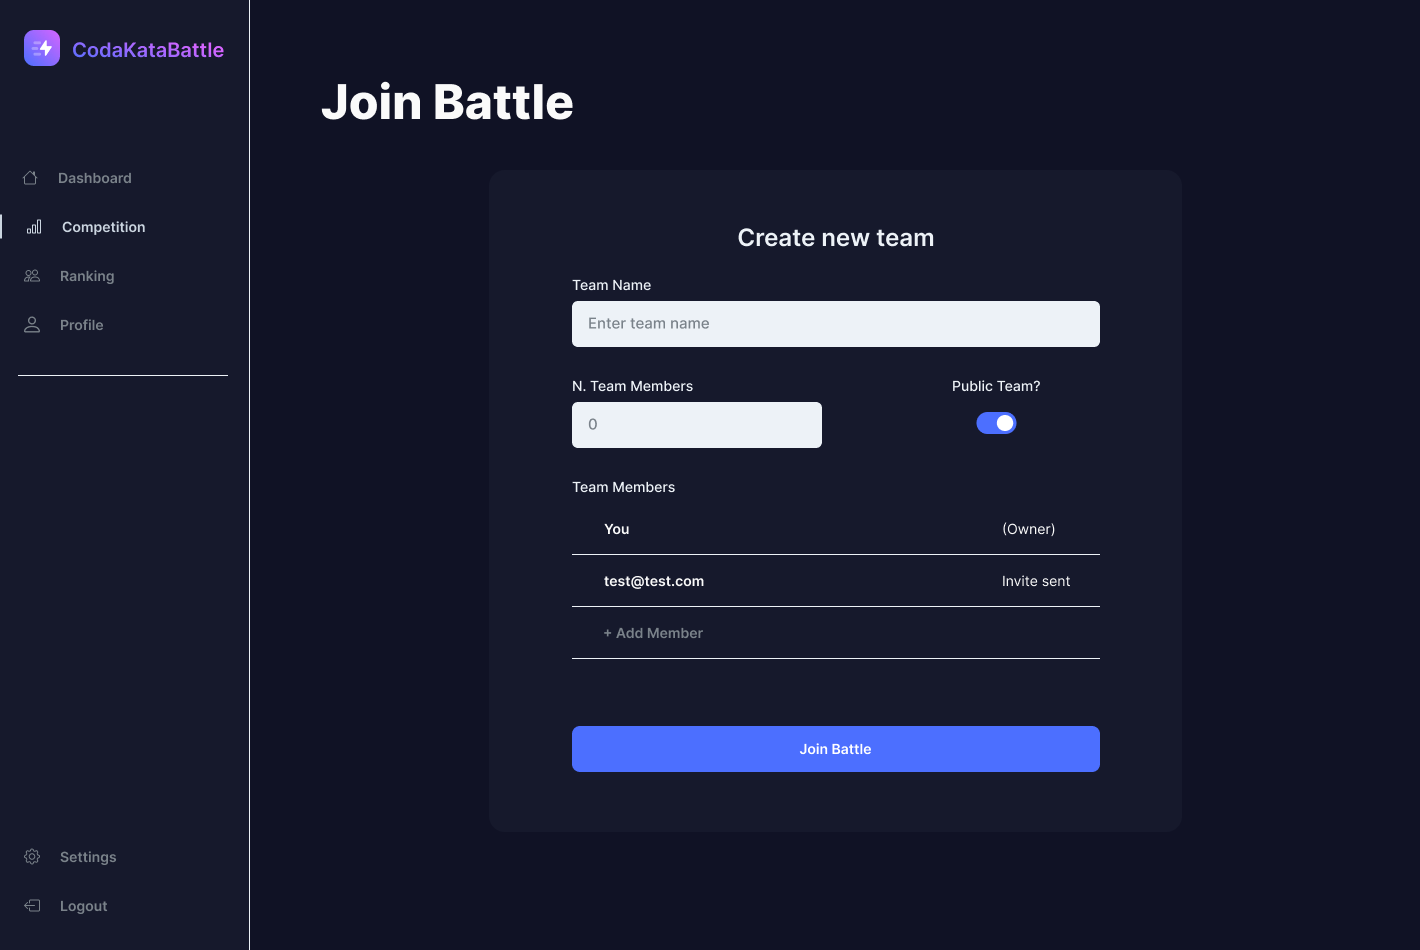
\includegraphics[width=0.95\textwidth]{User Interface/Join Battle Student - 3.png}
  \caption{Create a new team}
  \label{fig:join_battle3}
\end{figure}

\begin{figure}[H]
  \centering
  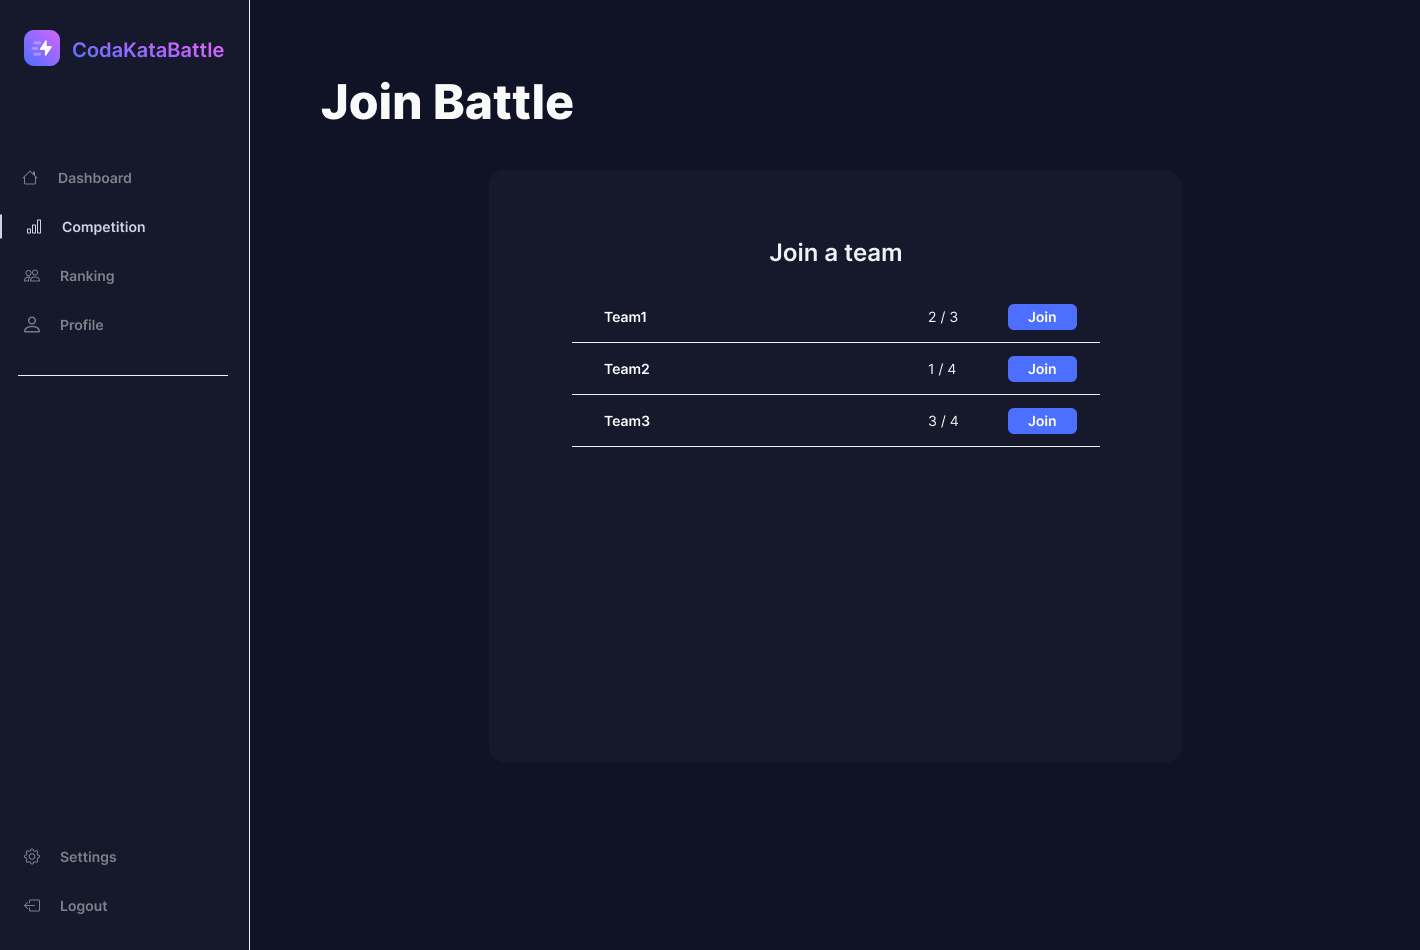
\includegraphics[width=\textwidth]{User Interface/Join Battle Student - 4.png}
  \caption{Join a public team}
  \label{fig:join_battle4}
\end{figure}

\newpage

\section*{ED Interfaces}
\label{s:ED_interface}%

In this section are presented the interfaces that are specific for the ED, in particular are shown the pages relative to the creation of a competition, the creation of a battle and the creation of a badge.

\subsubsection*{Create Competition Page}
\label{ss:create_competition_page}%

\begin{figure}[H]
  \centering
  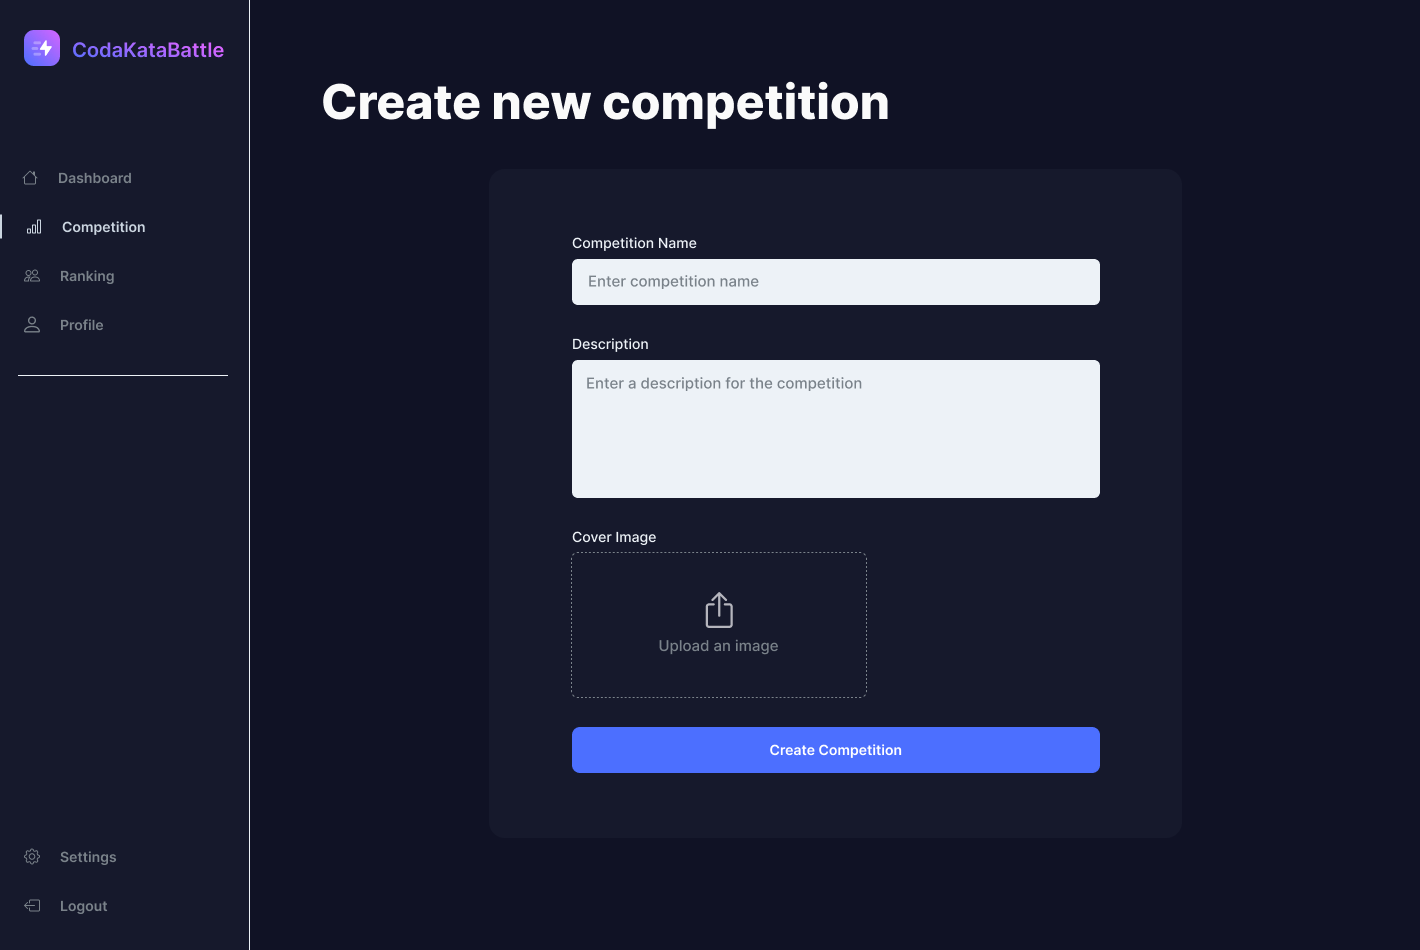
\includegraphics[width=\textwidth]{User Interface/Create Competition Educator.png}
  \caption{CKB create competition page}
  \label{fig:create_competition}
\end{figure}


\subsubsection*{Create Battle Pages}
\label{ss:create_battle_pages}%
As for the join of a battle for a ST also the creation of a battle is divided in two different steps. In the first step the ED has to insert all the general information about the battle, while in the second step he/her has to insert the code and settings for the automatic evaluation of the code.

\begin{figure}[H]
  \centering
  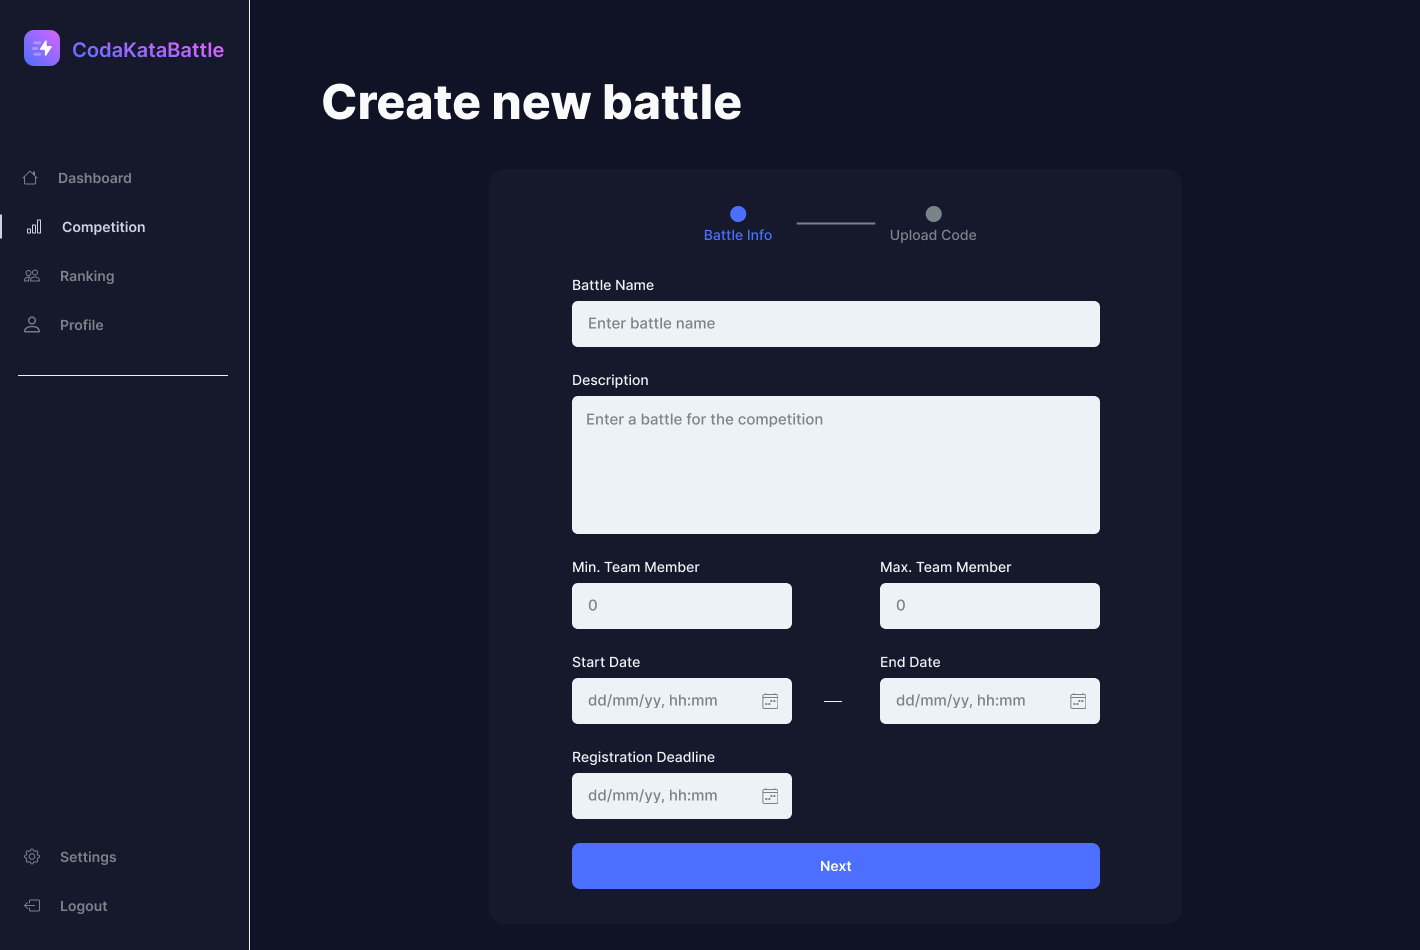
\includegraphics[width=0.95\textwidth]{User Interface/Create Battle Educator - 1.png}
  \caption{CKB create battle page - step 1}
  \label{fig:create_battle1}
\end{figure}

\begin{figure}[H]
  \centering
  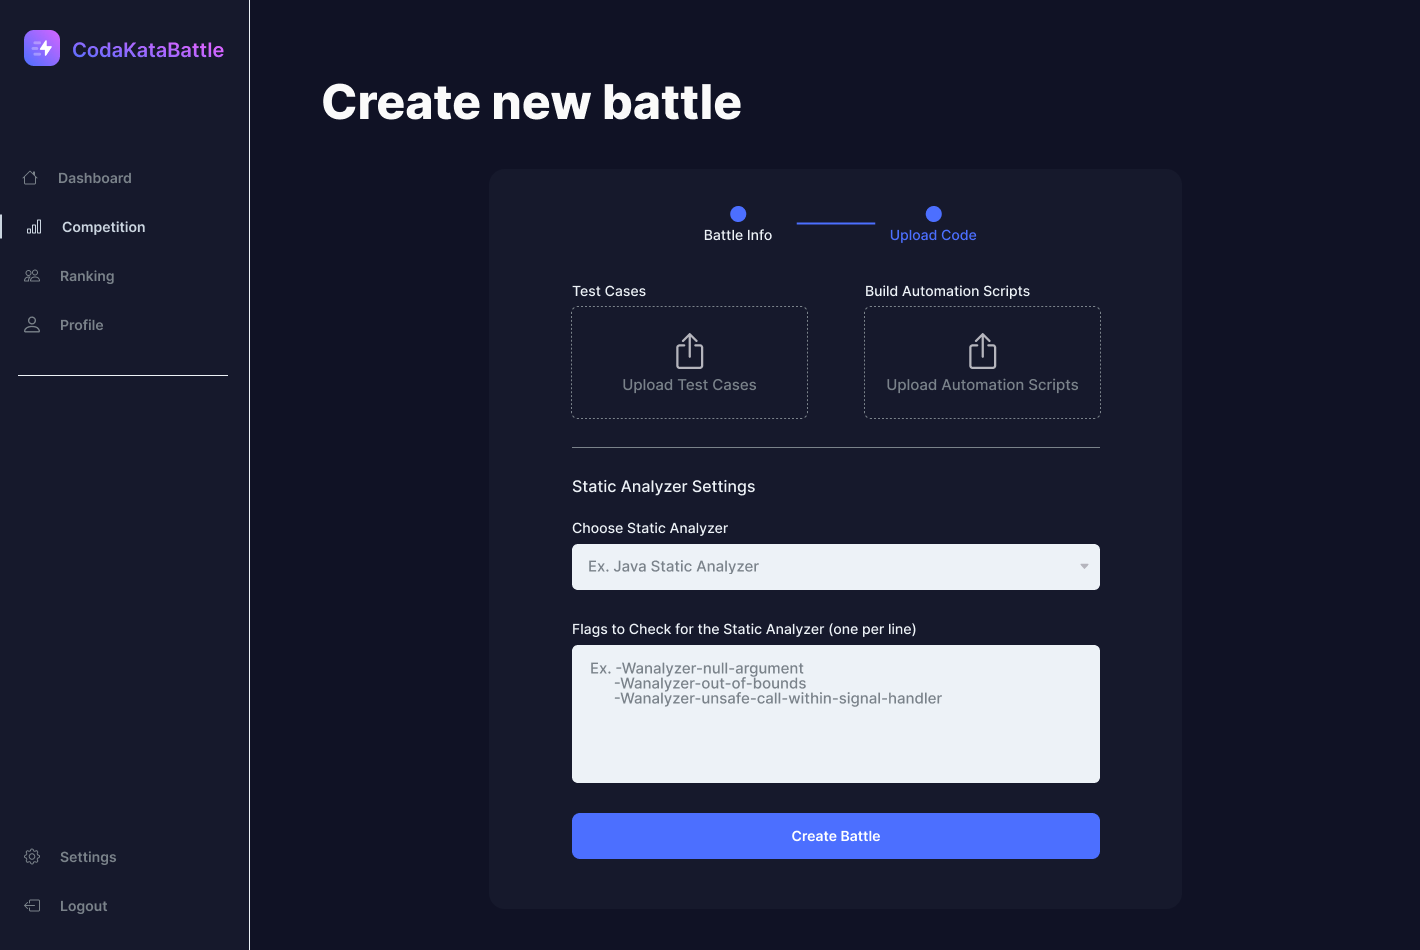
\includegraphics[width=0.95\textwidth]{User Interface/Create Battle Educator - 2.png}
  \caption{CKB create battle page - step 2}
  \label{fig:create_battle2}
\end{figure}


\subsubsection*{Create Badge Pages}
\label{ss:create_badge_pages}%
Similarly to the last function, the creation of a badge is divided in two steps. In the first step the ED can insert all the information of the badge, that include the name of the badge, a description and a picture. In the second step the ED can choose the criteria that the ST has to satisfy to earn the badge, this is done by a set of pre-defined criteria that the ED can choose from.

\begin{figure}[H]
  \centering
  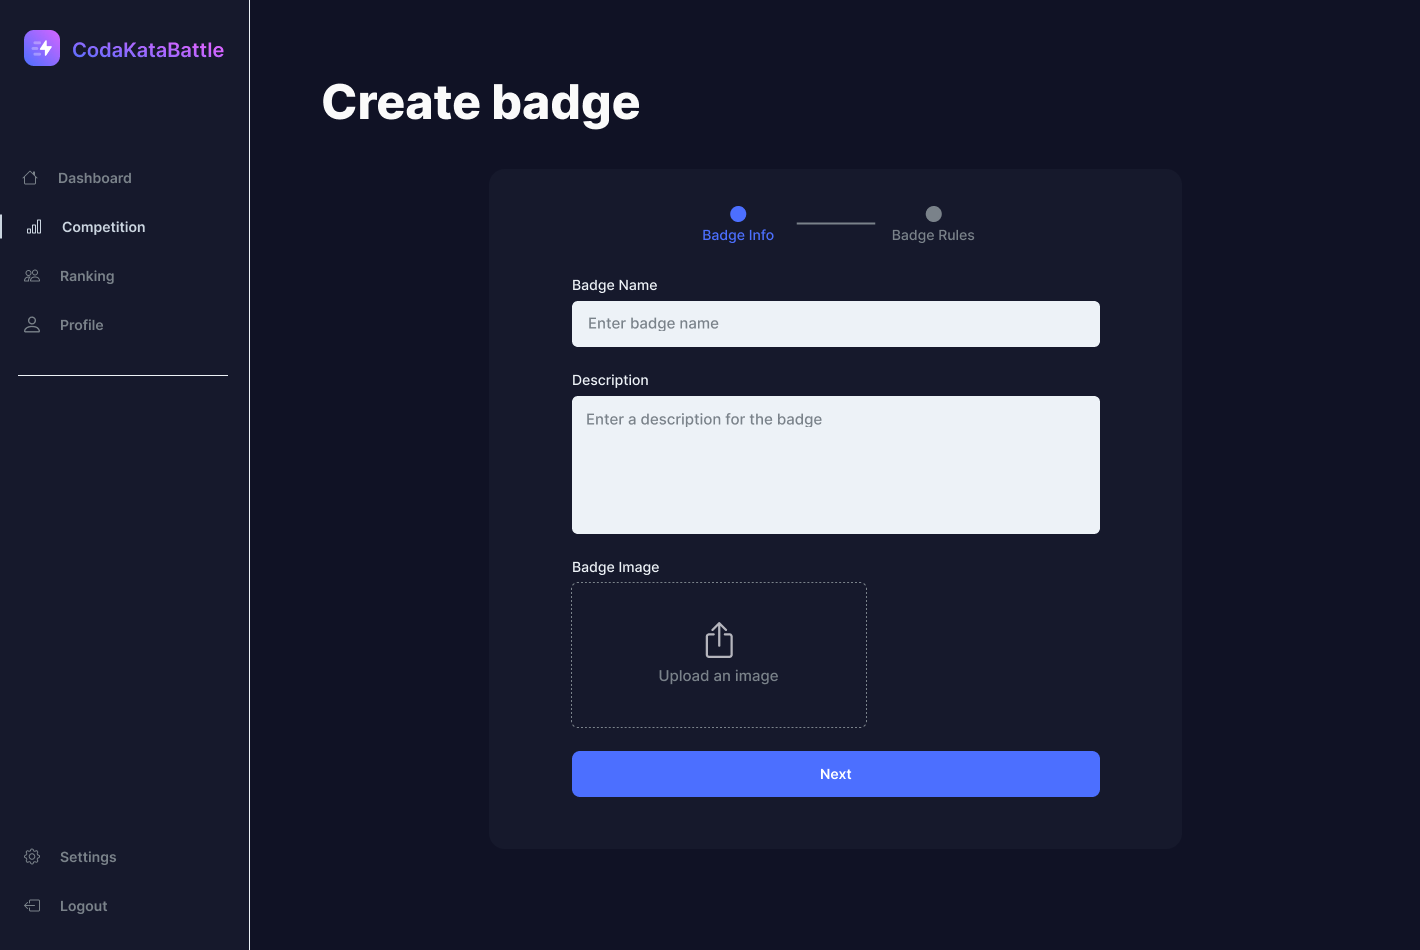
\includegraphics[width=\textwidth]{User Interface/Create Badge Educator - 1.png}
  \caption{CKB create badge page - step 1}
  \label{fig:create_badge1}
\end{figure}

\begin{figure}[H]
  \centering
  \includegraphics[width=\textwidth]{User Interface/Create badge Educator - 2.png}
  \caption{CKB create badge page - step 2}
  \label{fig:create_badge2}
\end{figure}

\newpage

\subsubsection*{Manual Evaluation Page}
\label{ss:manual_evaluation_page}%
This is the page where the ED can manually evaluate the code of a T. In particular, the ED can see some information about the latest submission of a T and can visit GitHub to see the code of the T. Then the ED can evaluate the latest submission of the T, assigning a score.

\begin{figure}[H]
  \centering
  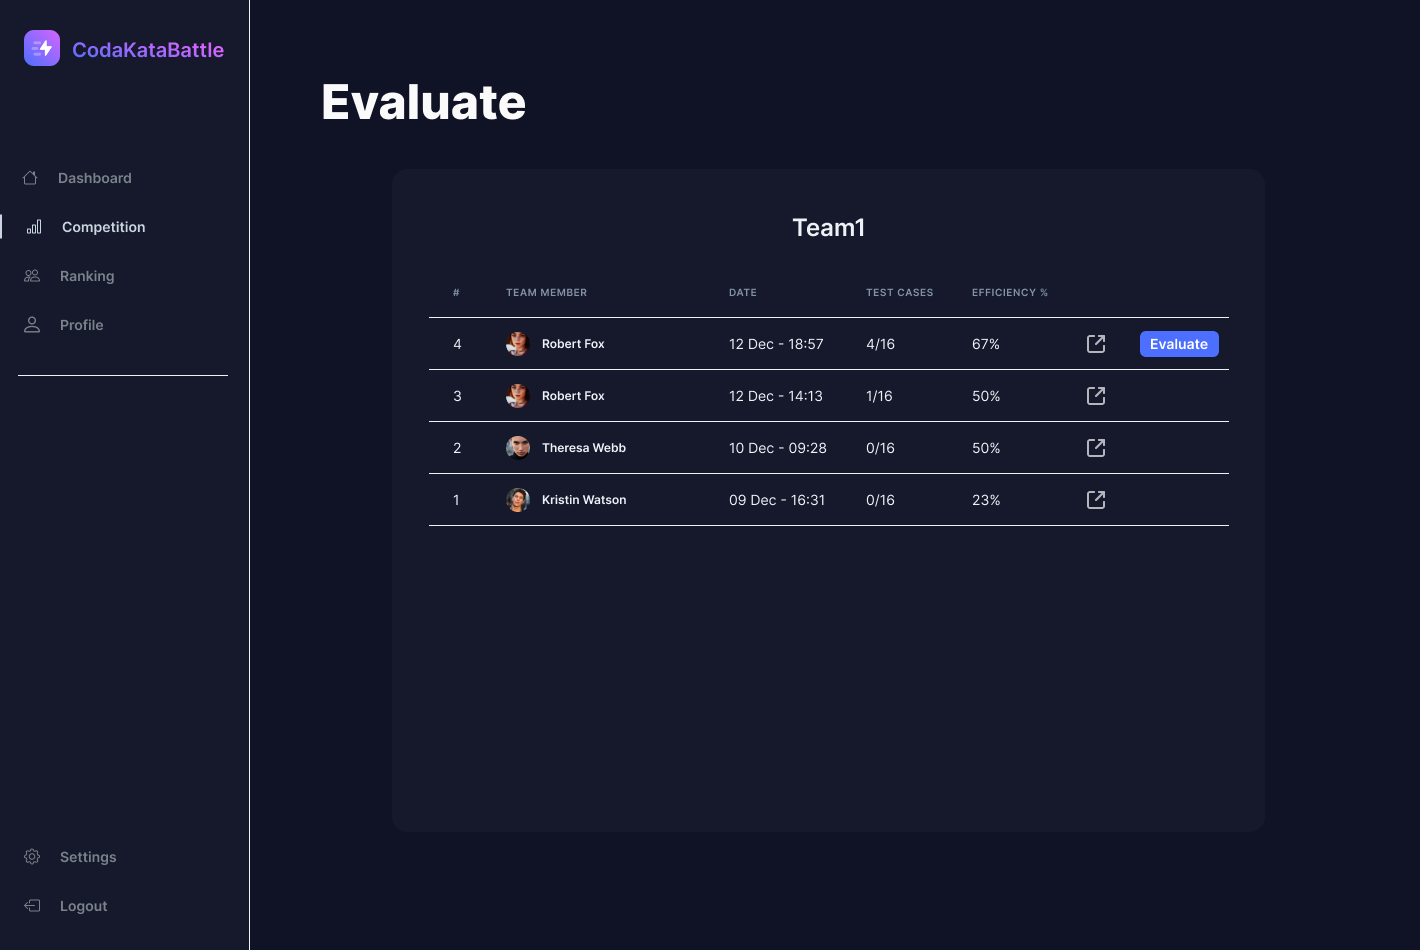
\includegraphics[width=\textwidth]{User Interface/Manual Evaluation Educator.png}
  \caption{CKB manual evaluation page}
  \label{fig:manual_evaluation}
\end{figure}




%-------------------------------------------------------------------------
%	Requirements traceability
%-------------------------------------------------------------------------
\chapter{Requirements traceability}
\label{c:requirements_traceability}%
%


%-------------------------------------------------------------------------
%	Implementation, integration and test plan
%-------------------------------------------------------------------------
\chapter{Implementation, integration and test plan}
\label{c:implementation_integration_test_plan}%
The implementation, integration and test plan will follow a \textbf{bottom-up approach},
starting from the components with no dependencies and then integrating them together.

\section{Plan Definition}
Since the application is mostly server-side, we will only describe the implementation of the server components.
The client-side, which is actually a presentation layer, will be implemented and tested in parallel with the server-side.

Since our application is developed on two different servers, we will describe separately 
the implementation plan for the two servers: the \textit{CKB Server} and the \textit{Evaluation Server}.
\subsubsection{CKB Server}

In the first step, the \textit{Model} component and the \textit{Data Manager}, will be implemented and unit 
tested with a \textit{Driver} which will substitute components which are not already implemented.

\begin{figure}[H]
    \label{fig:step1-CKBServer}
    \centering
    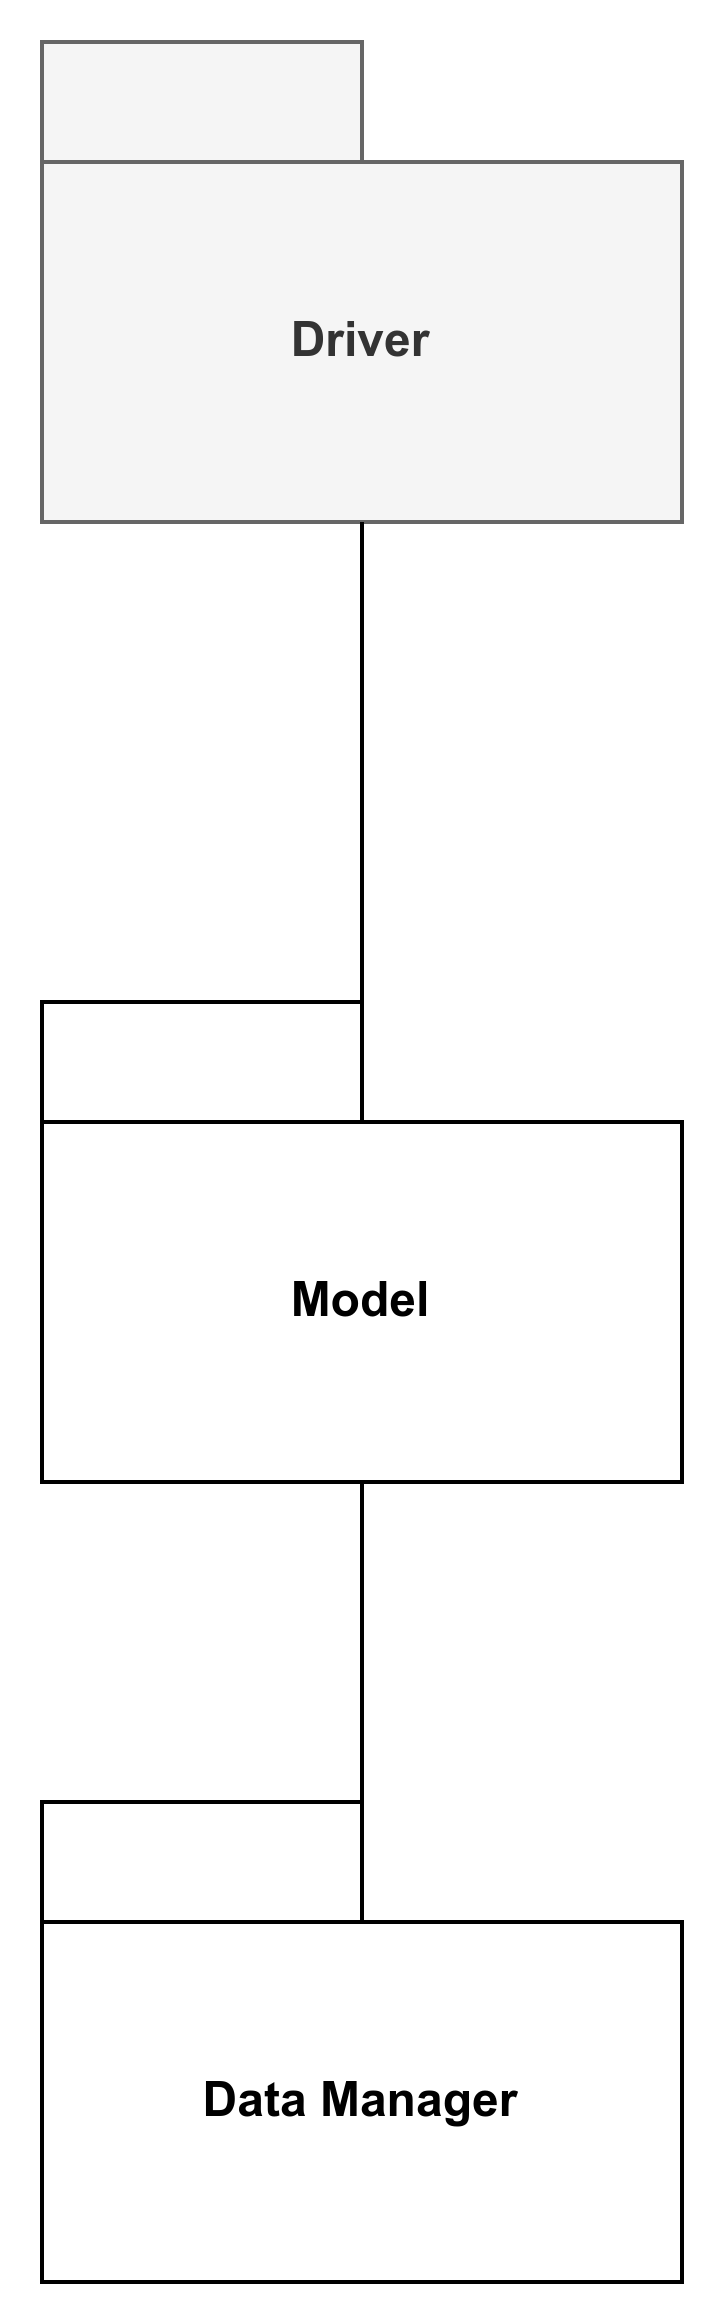
\includegraphics[height=0.5\textheight]{ImplementationStrategy/1_01-CKBServer.png}
    \caption{Step 1}
\end{figure}
In the second step, the Notification Manager will be implemented and tested with a \textit{Driver} which will substitute: 
the \textit{CompetitionManager},the \textit{BattleManager} and the \textit{AuthenticationService}.
It will also use a \textit{Stub} to simulate the \textit{Mail Server}.
\begin{figure}[H]
    \label{fig:step2-CKBServer}
    \centering
    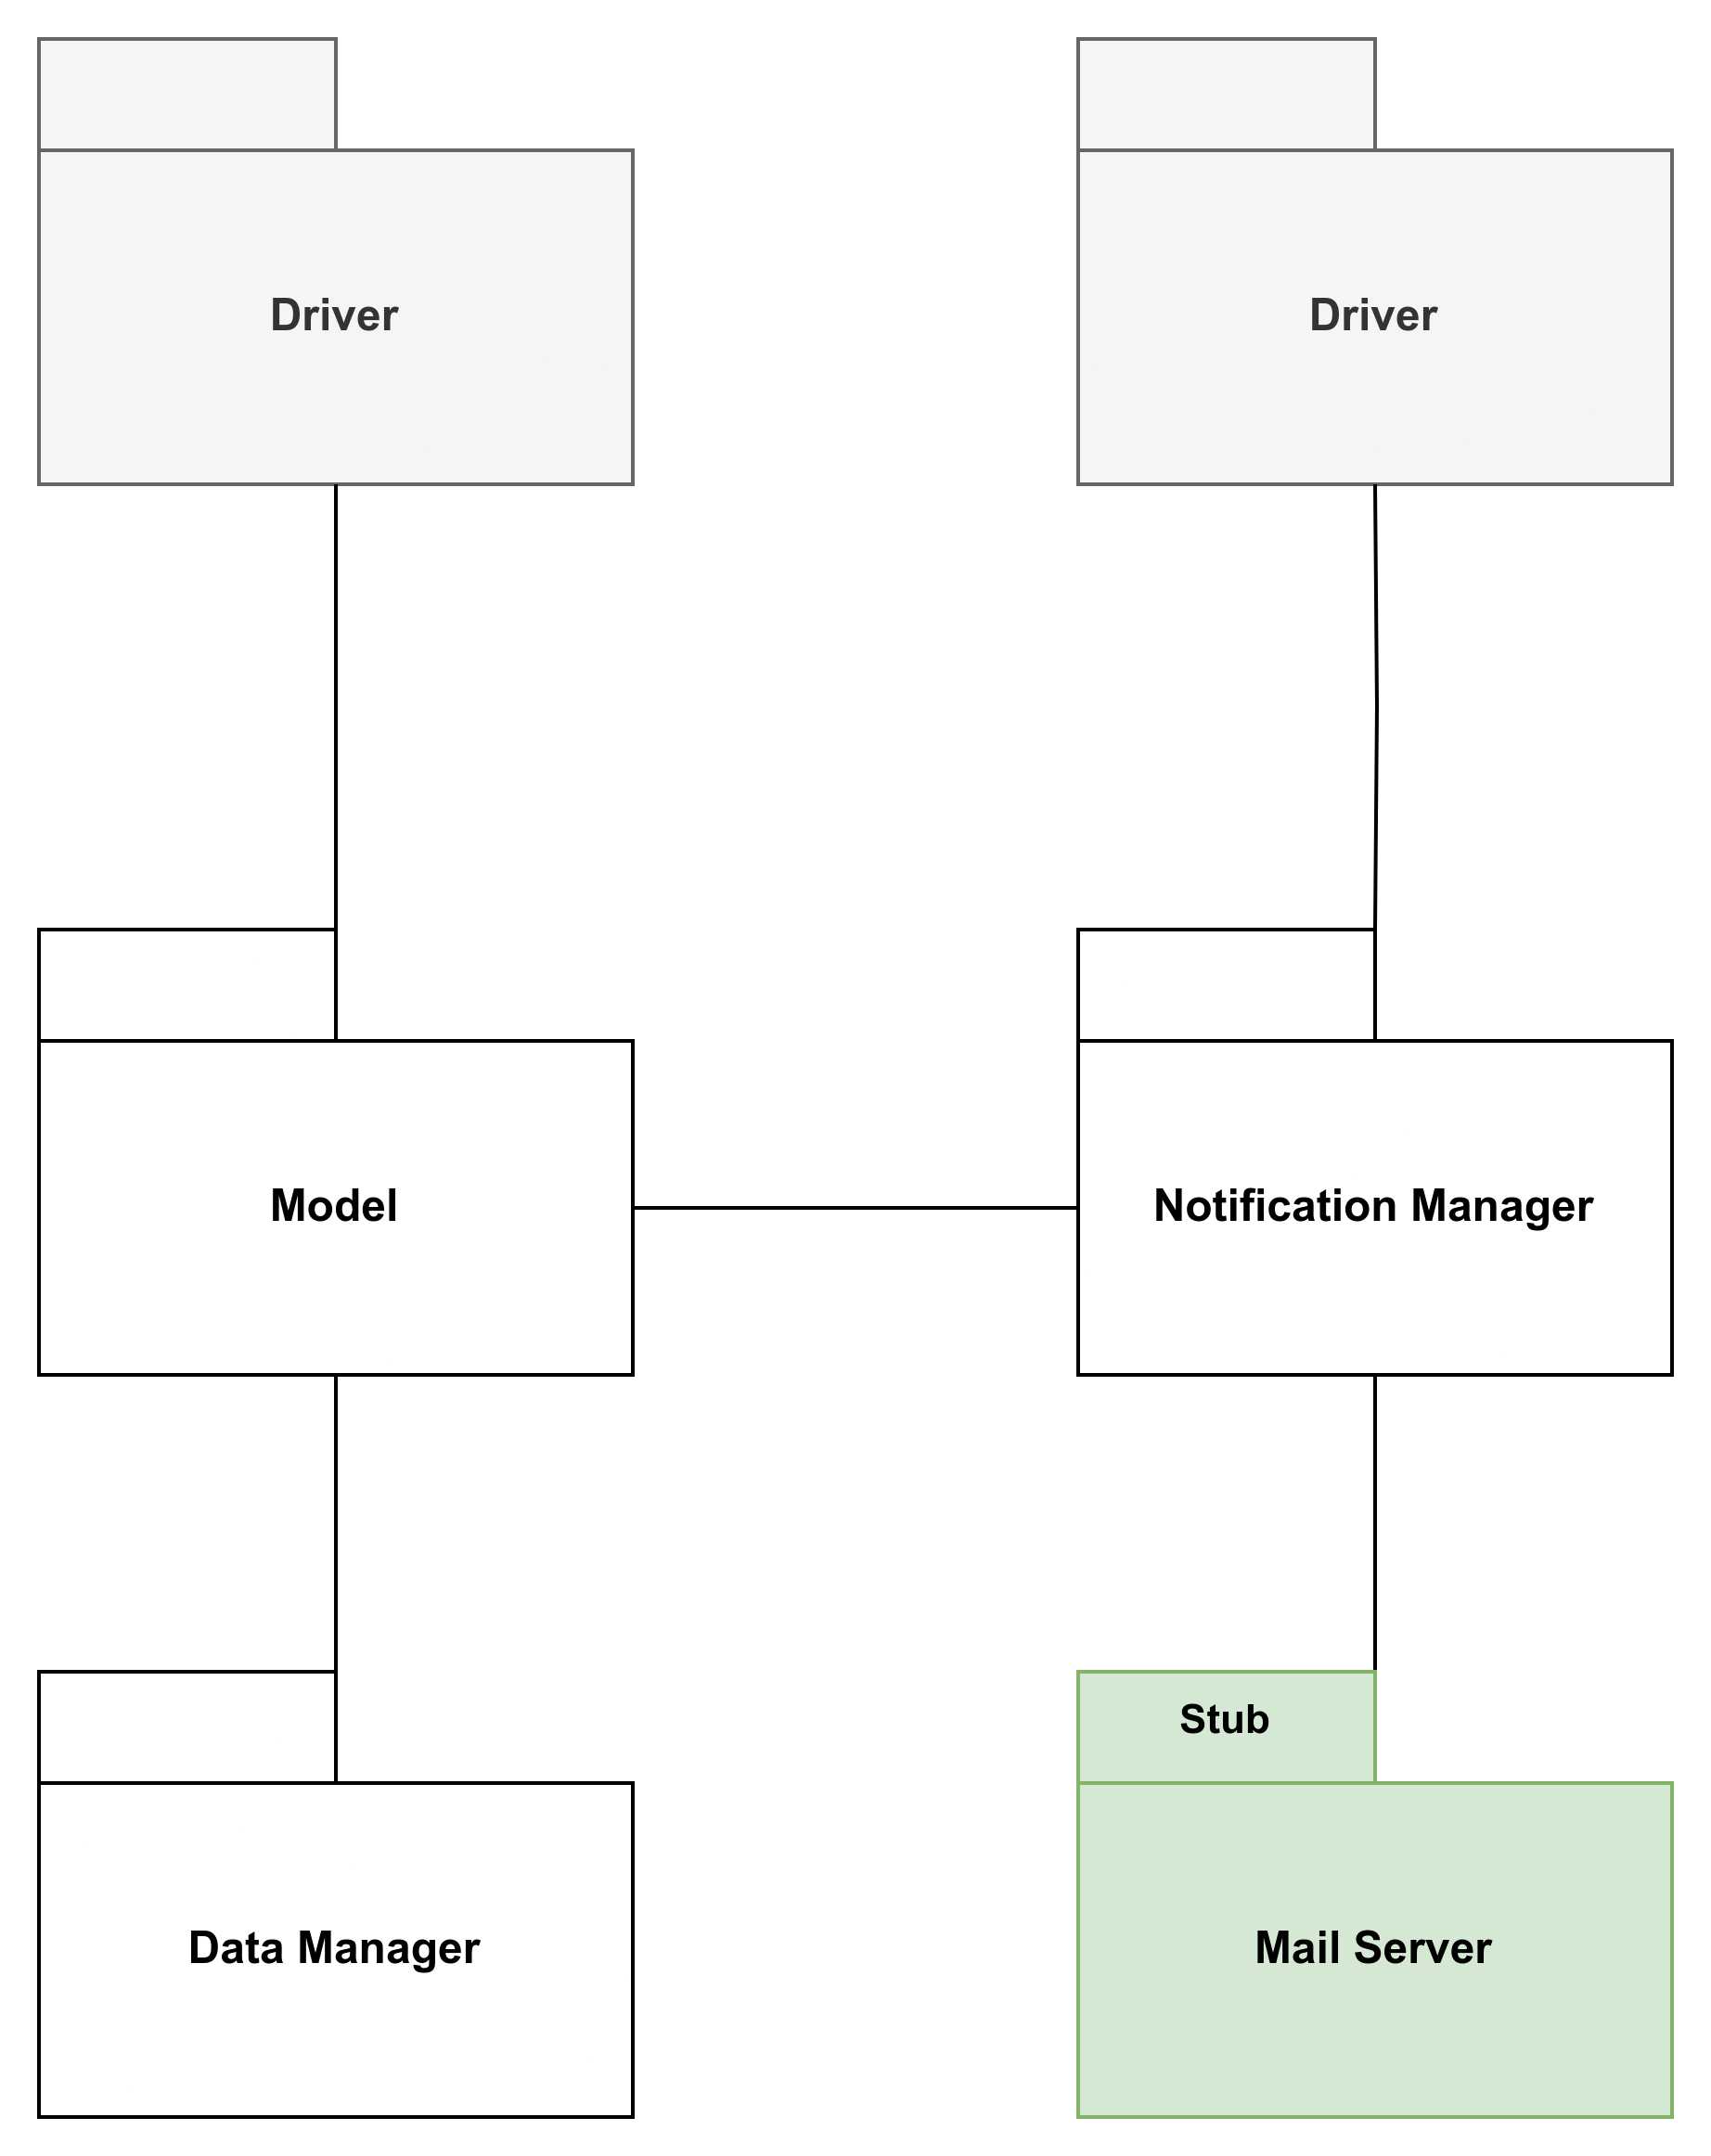
\includegraphics[height=0.5\textheight]{ImplementationStrategy/1_02-CKBServer.png}
    \caption{Step 2 - CKB Server}
\end{figure}

\begin{figure}[H]
    \label{fig:step3-CKBServer}
    \centering
    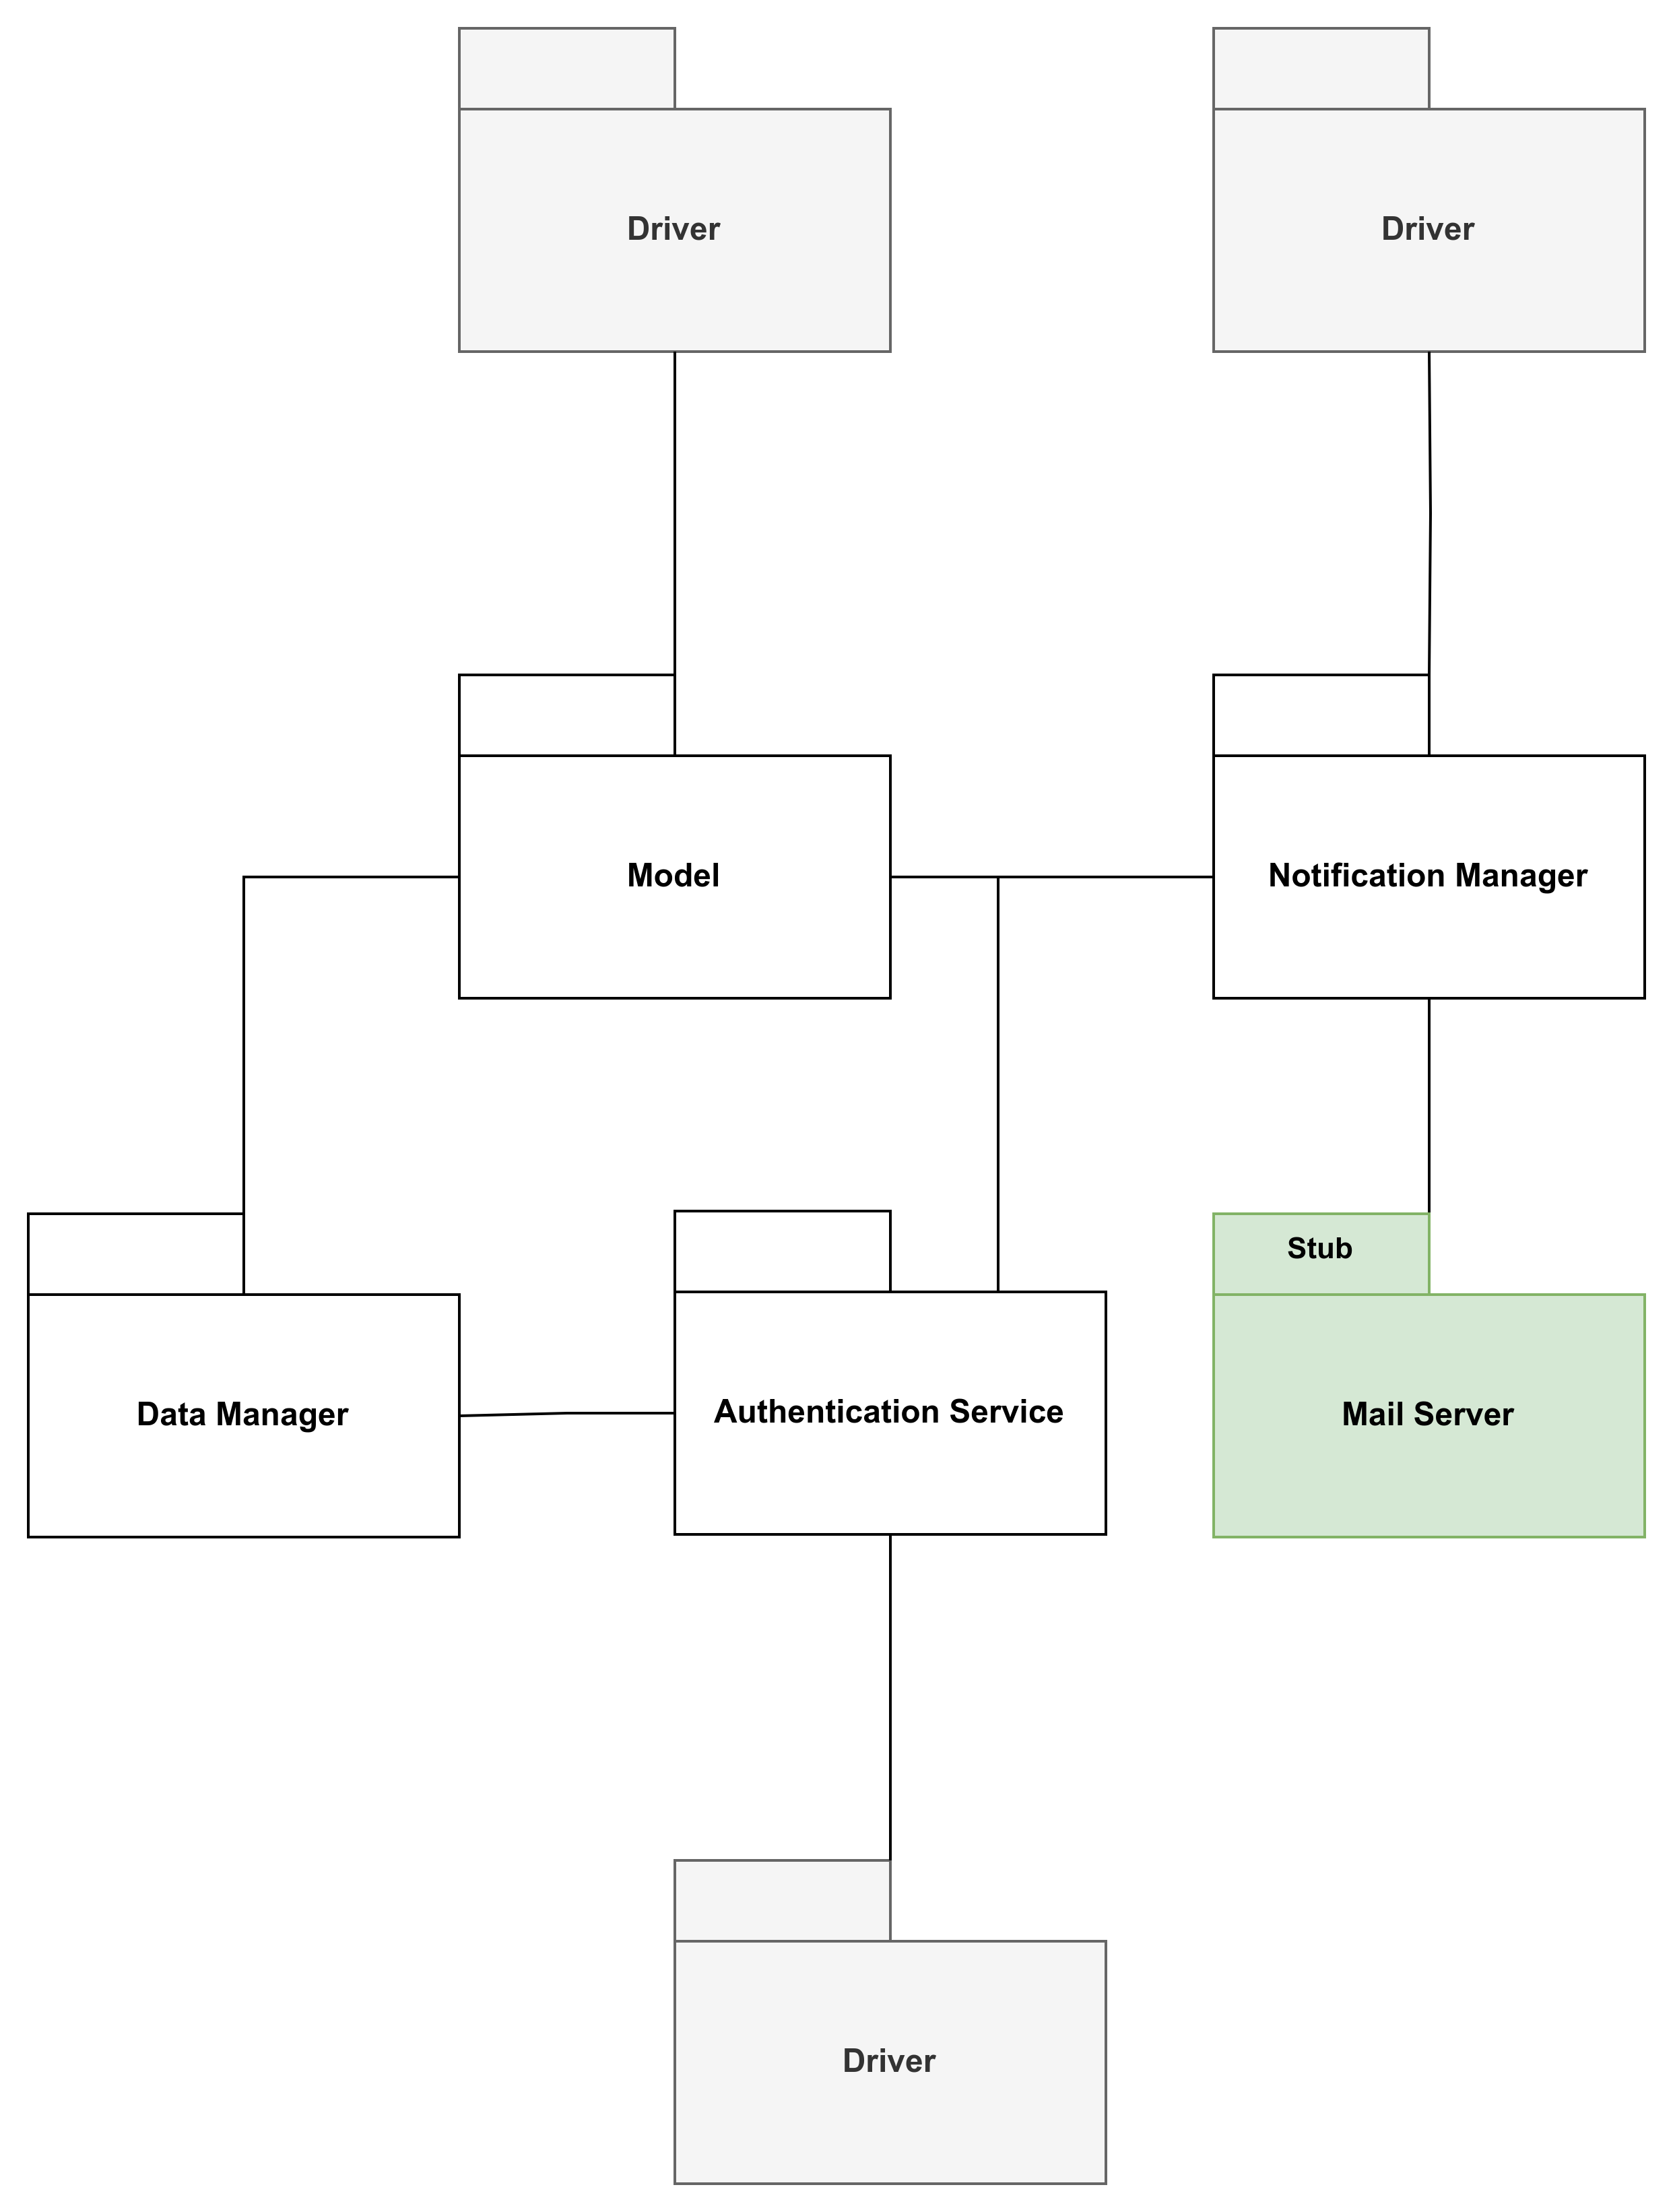
\includegraphics[height=0.5\textheight]{ImplementationStrategy/1_03-CKBServer.png}
    \caption{Step 3 - CKB Server}
\end{figure}


\begin{figure}[H]
    \label{fig:step4-CKBServer}
    \centering
    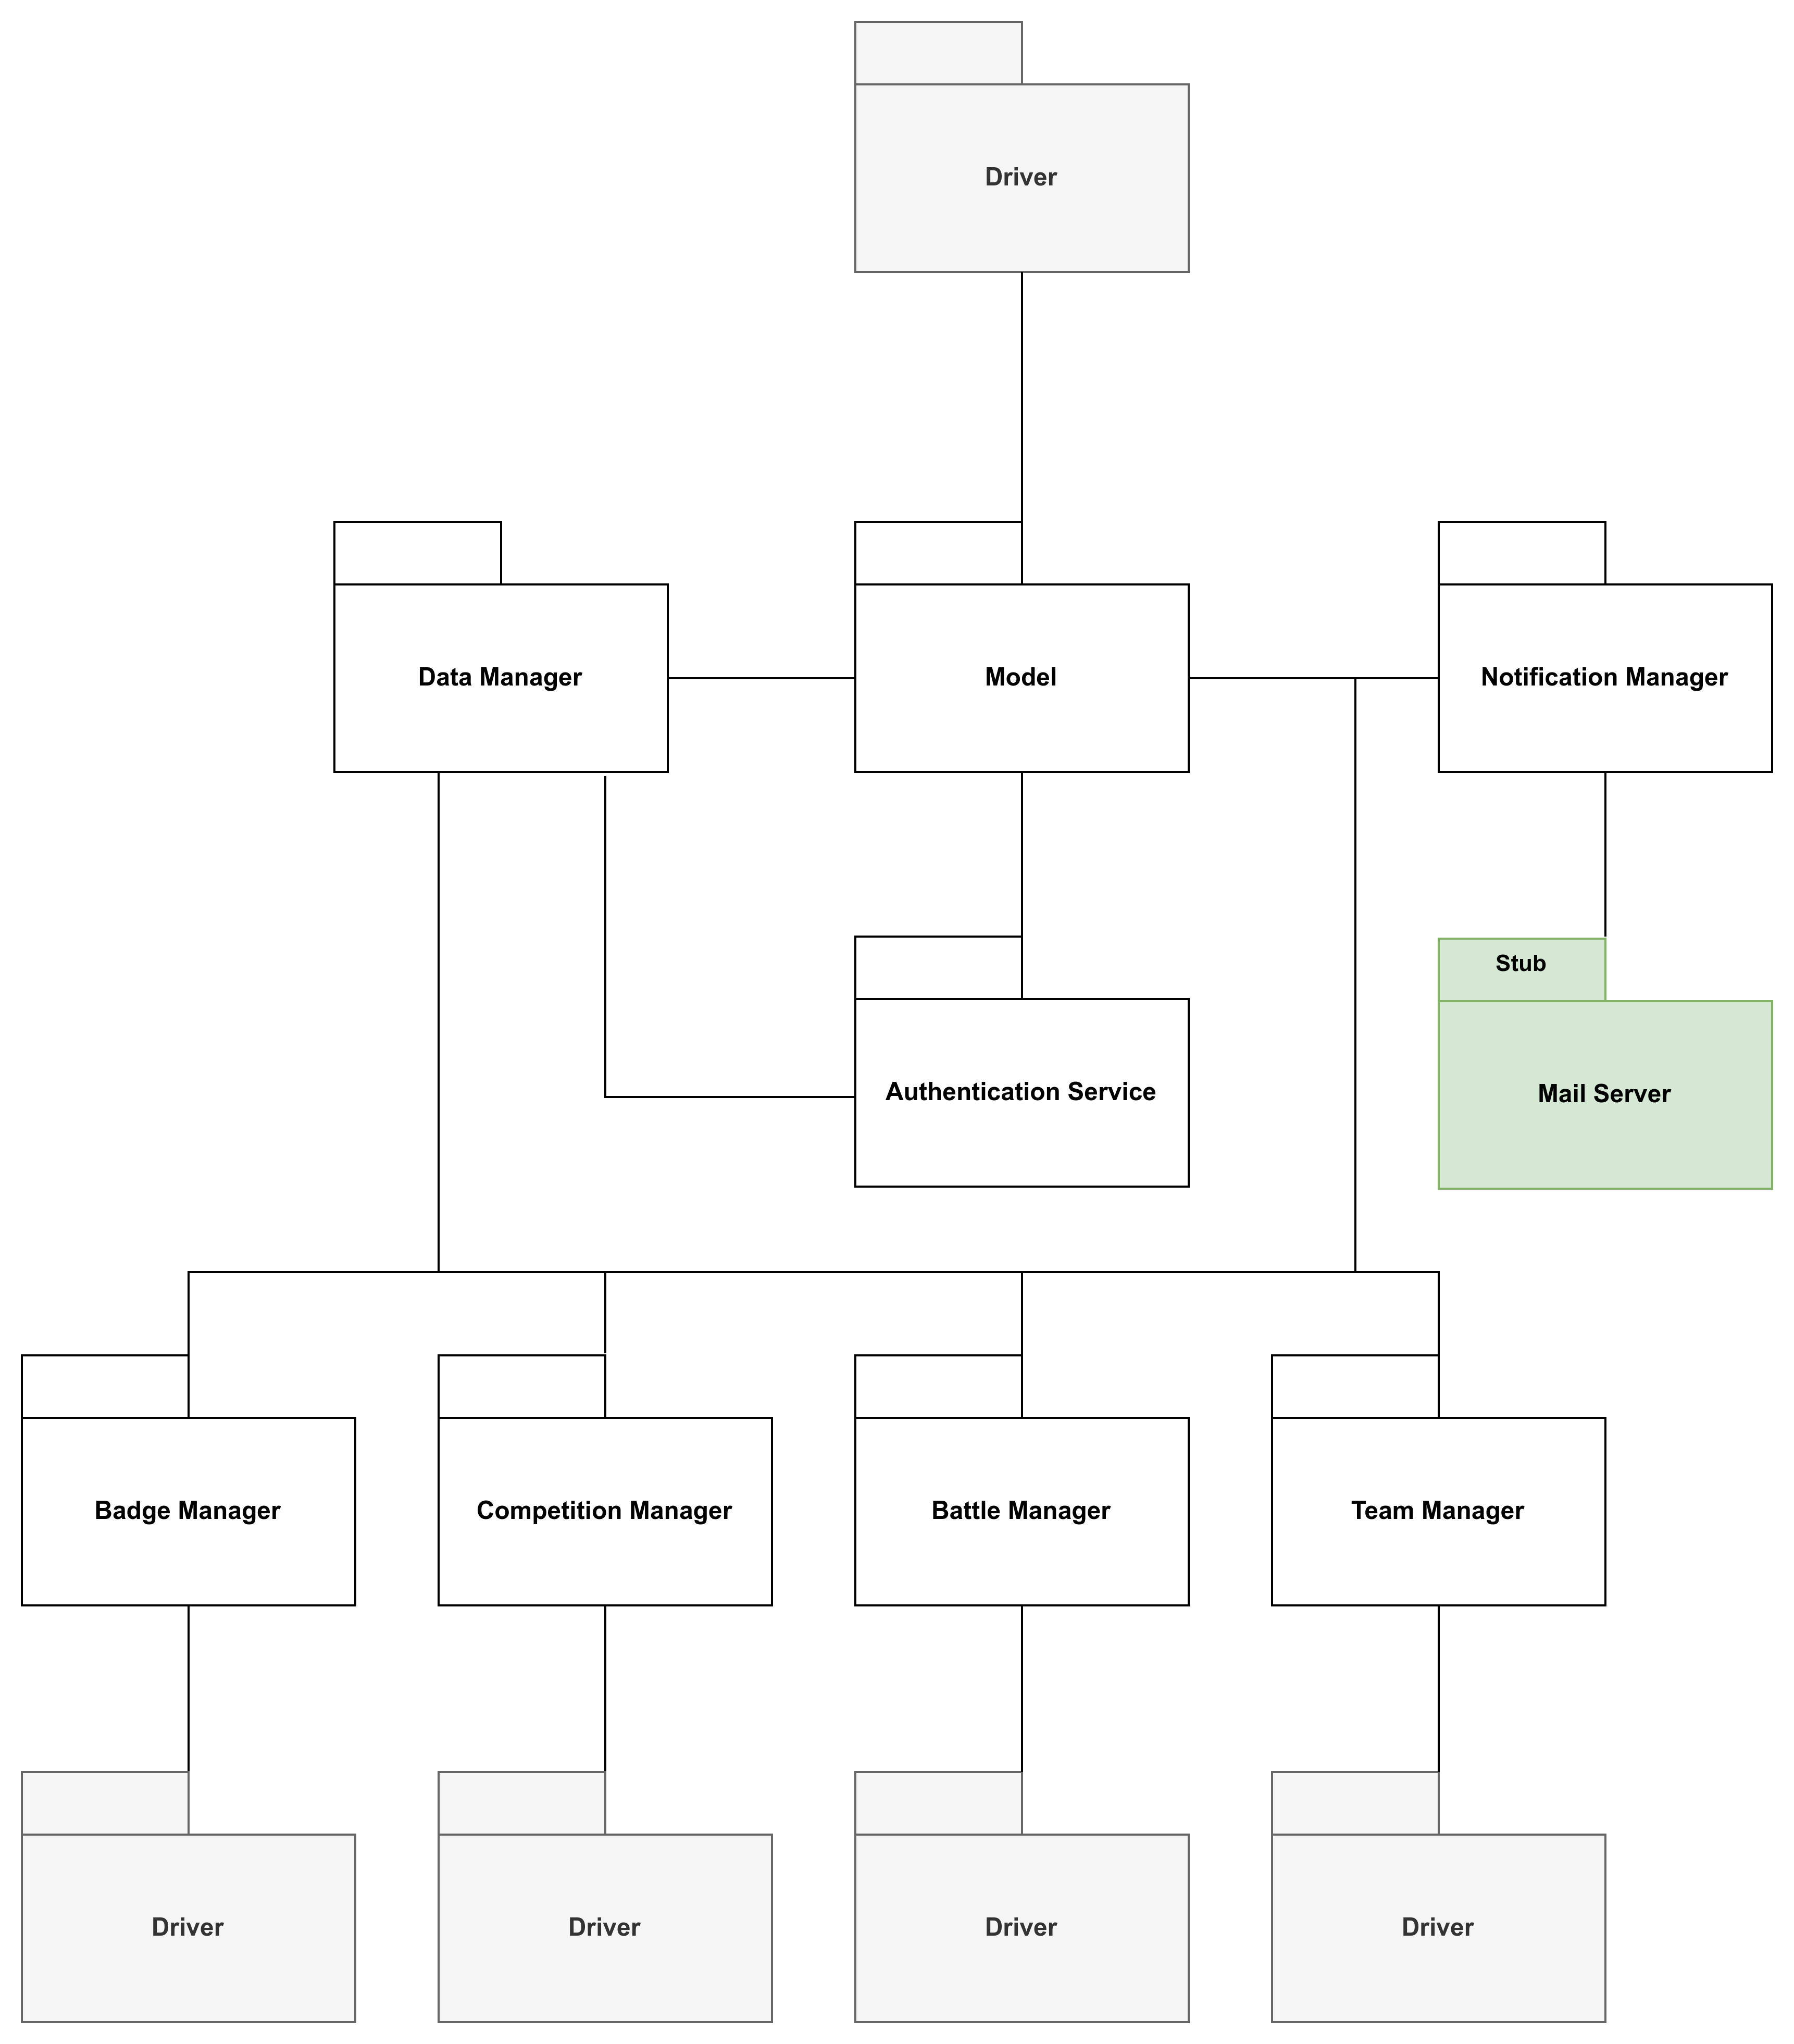
\includegraphics[height=0.8\textheight]{ImplementationStrategy/1_04-CKBServer.png}
    \caption{Step 4 - CKB Server}
\end{figure}


\begin{figure}[H]
    \label{fig:step5-CKBServer}
    \centering
    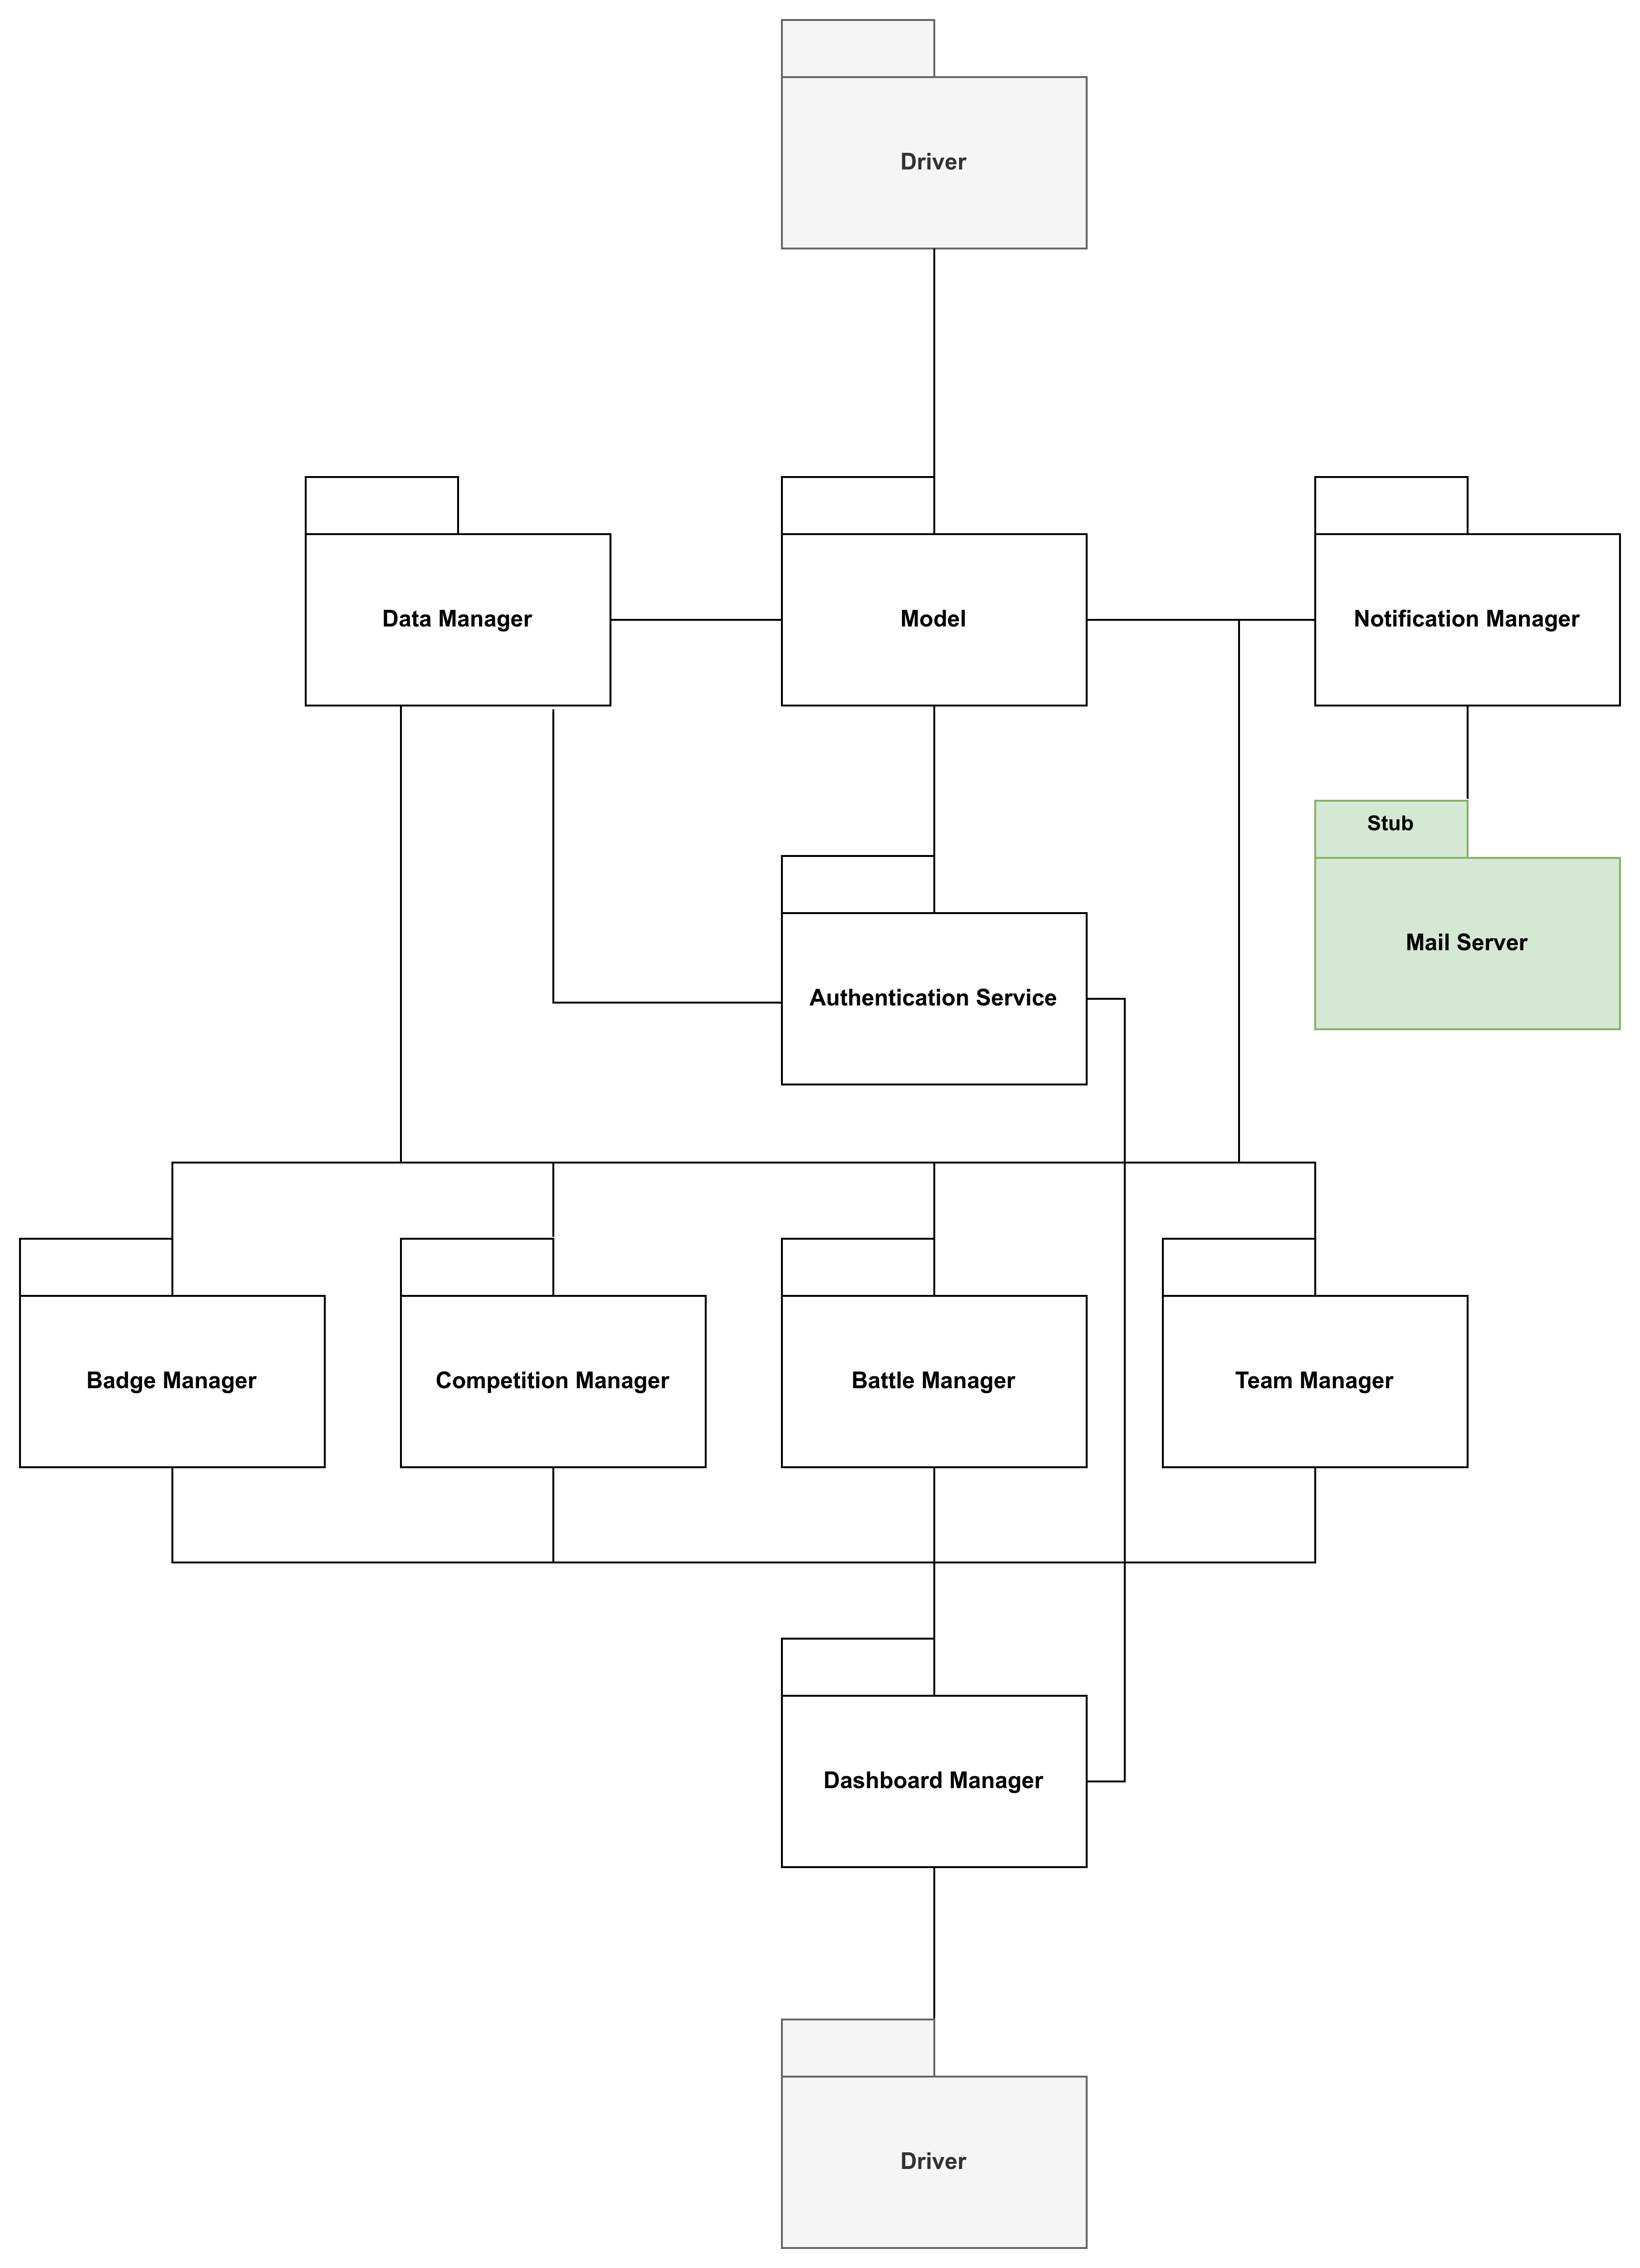
\includegraphics[height=0.8\textheight]{ImplementationStrategy/1_05-CKBServer.png}
    \caption{Step 5 - CKB Server}
\end{figure}


\subsubsection{Evaluation Server}

\begin{figure}[H]
    \label{fig:step1-EvaluationServer}
    \centering
    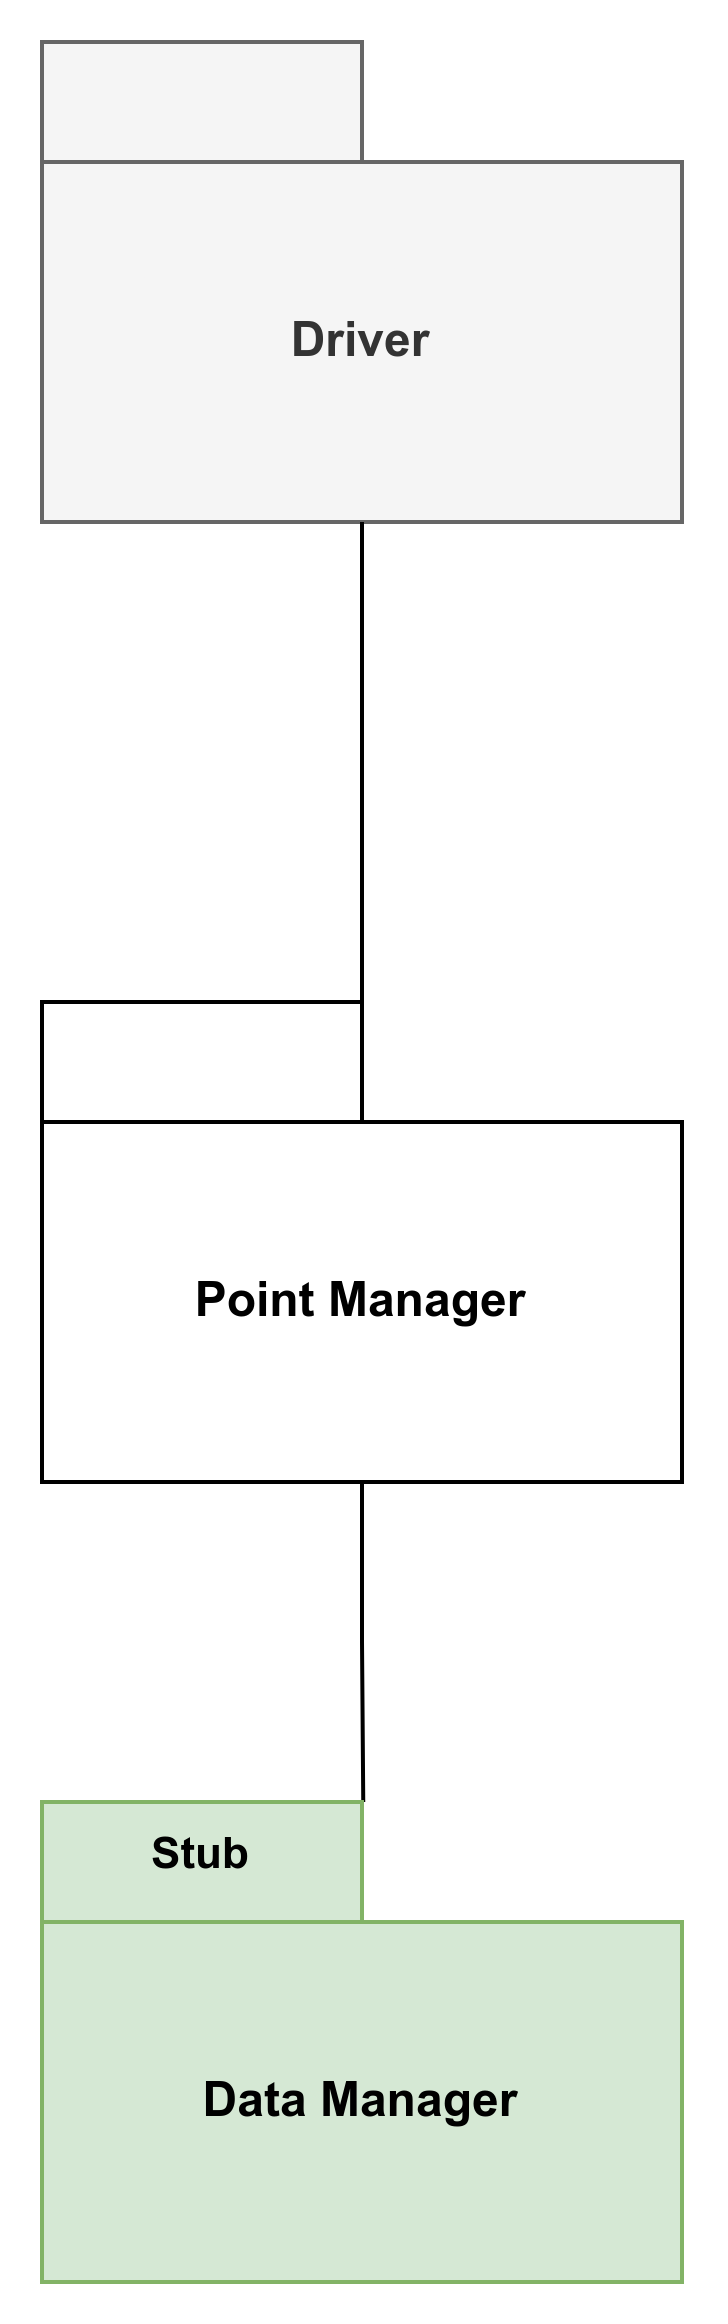
\includegraphics[height=0.5\textheight]{ImplementationStrategy/2_01-EvaluationServer.png}
    \caption{Step 1 - Evaluation Server}
\end{figure}

\begin{figure}[H]
    \label{fig:step2-EvaluationServer}
    \centering
    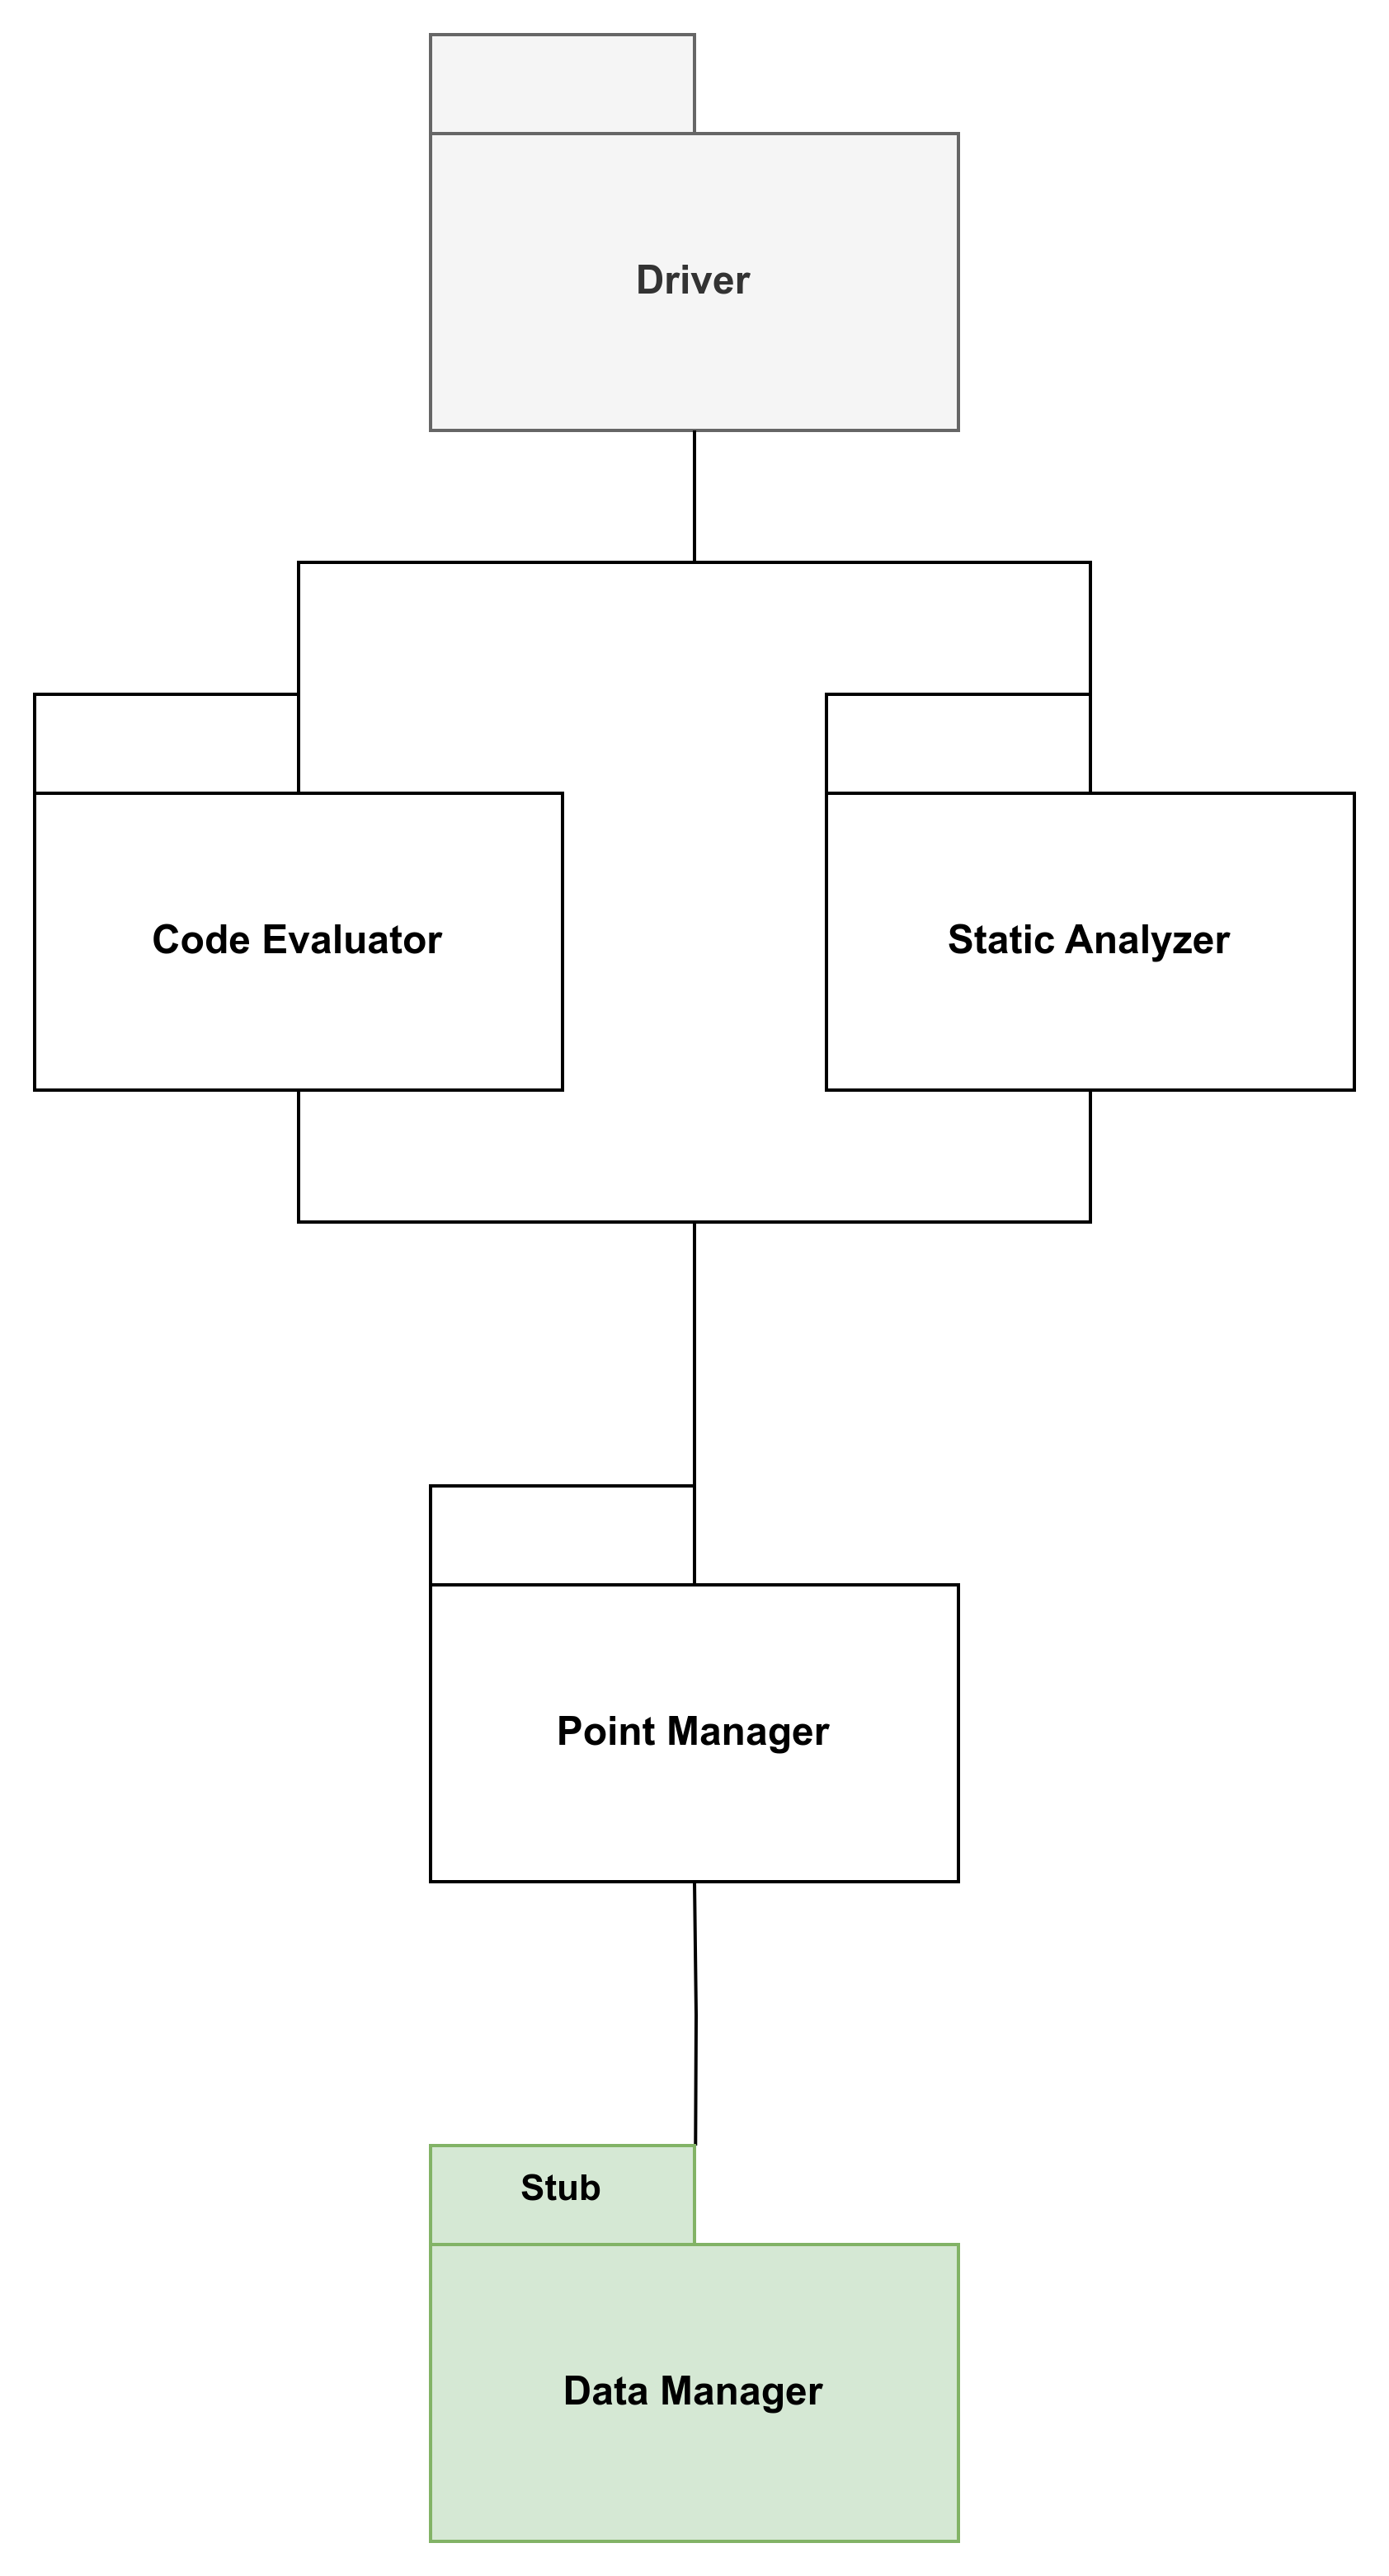
\includegraphics[height=0.5\textheight]{ImplementationStrategy/2_02-EvaluationServer.png}
    \caption{Step 2 - Evaluation Server}
\end{figure}

\begin{figure}[H]
    \label{fig:step3-EvaluationServer}
    \centering
    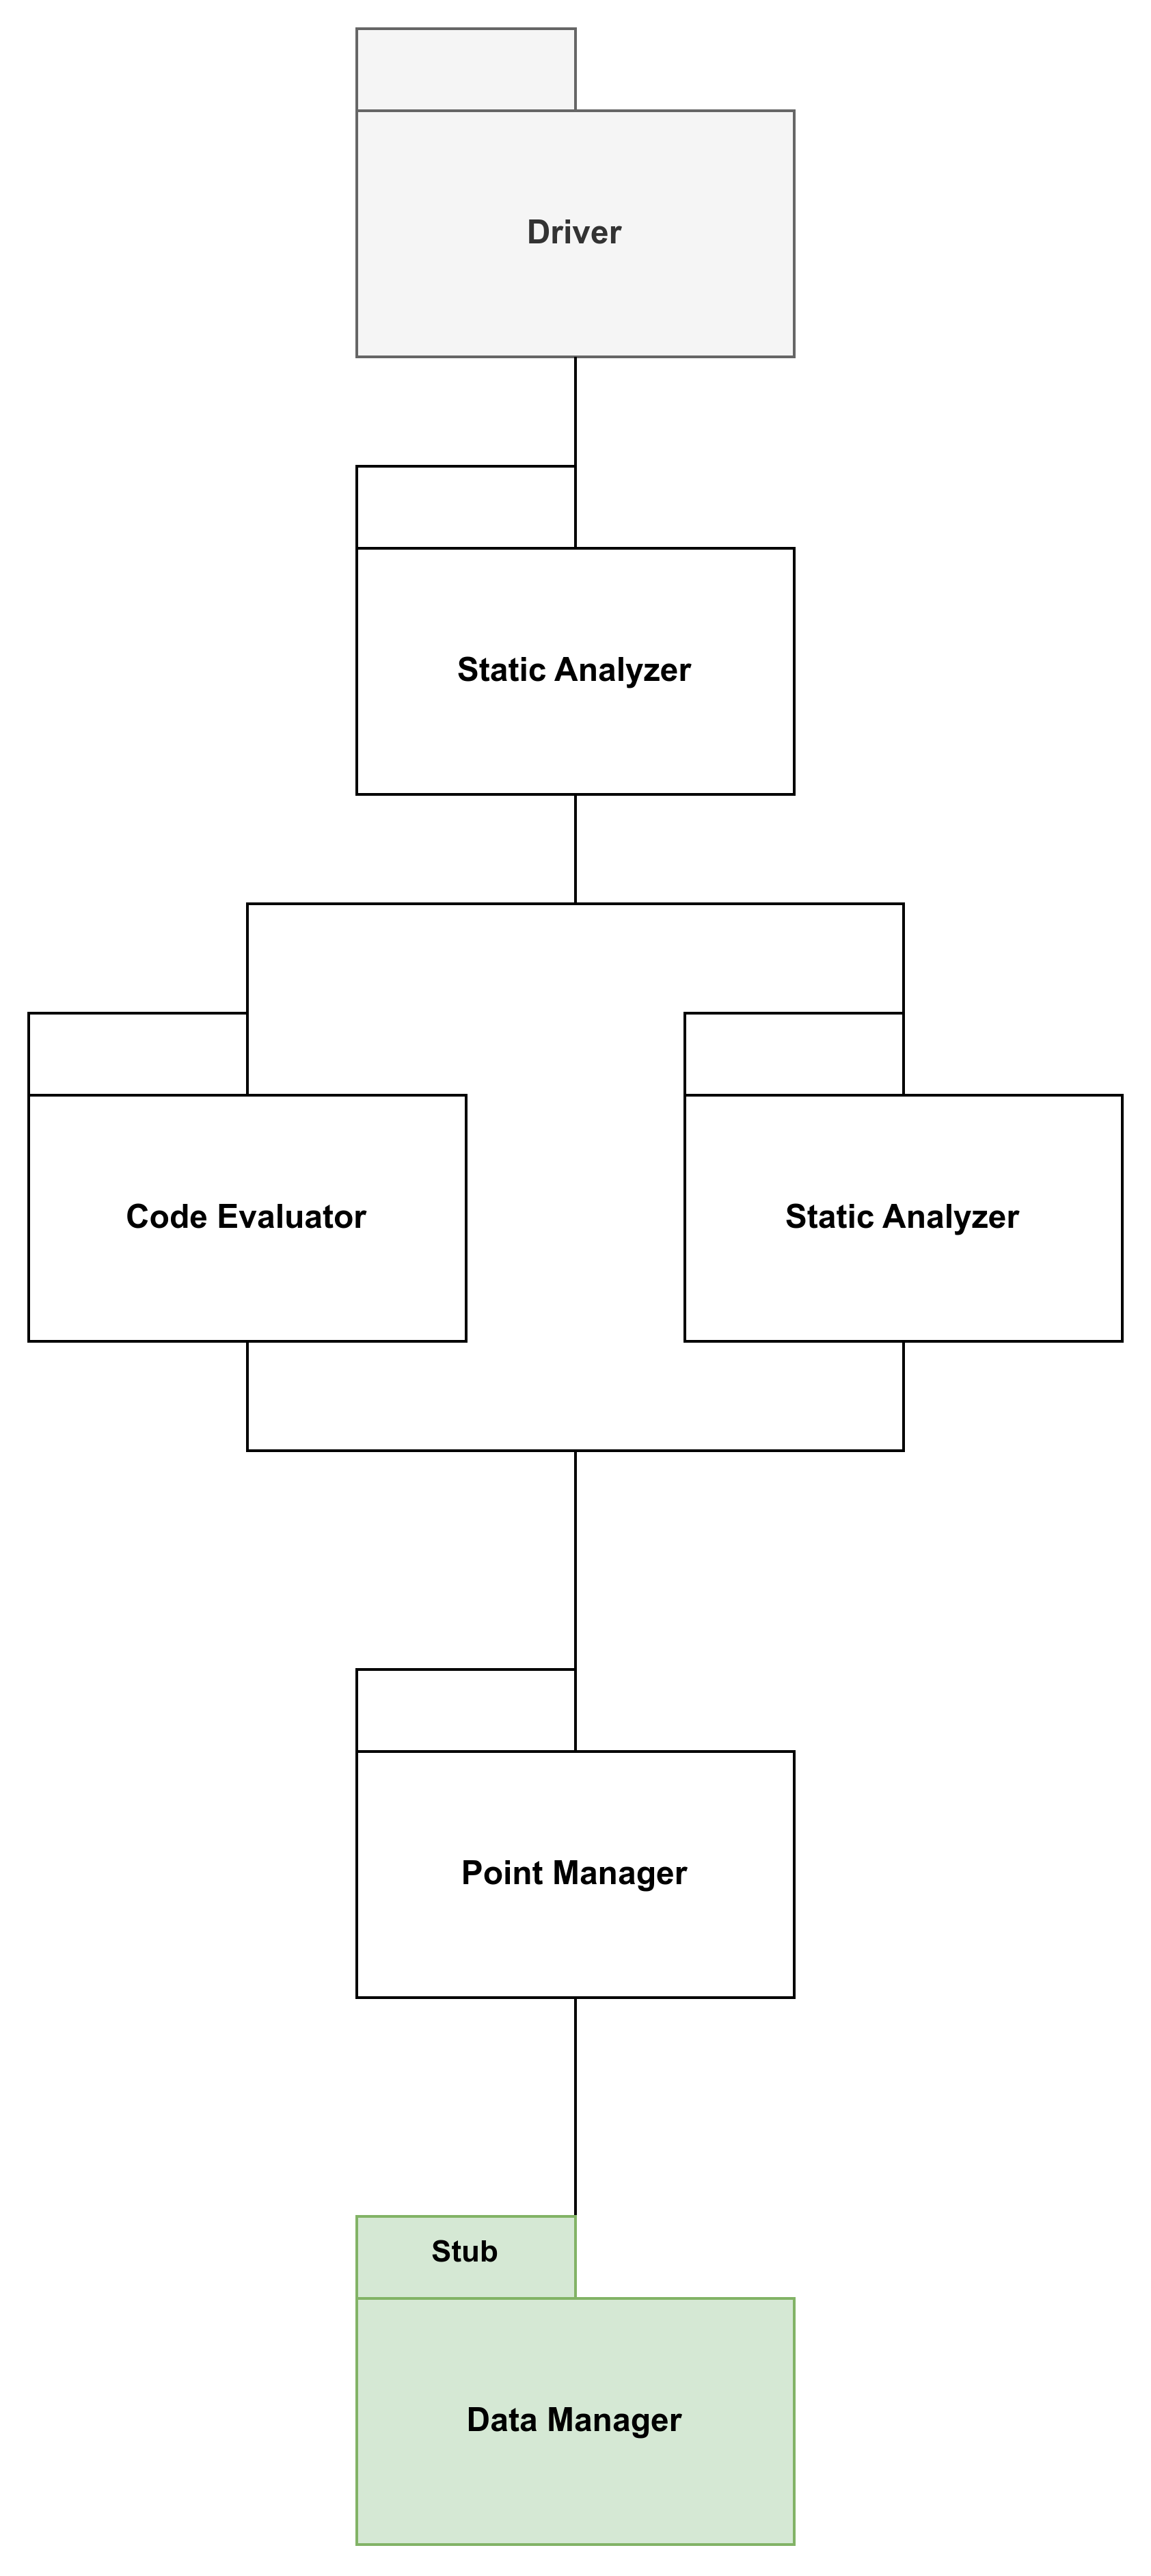
\includegraphics[height=0.5\textheight]{ImplementationStrategy/2_03-EvaluationServer.png}
    \caption{Step 3 - Evaluation Server}
\end{figure}


%-------------------------------------------------------------------------
%	Effort Spent
%----------------------------------------------------------------------
\chapter{Effort Spent}
\label{c:effort}%
\begin{table}[H]
  \centering
  \begin{tabular}{|l|l|}
    \hline
    \textbf{Members of group} & \textbf{Effort spent (hours)} \\ 
    \hline
    Filippo Balzarini & \begin{tabular}{p{0.25\linewidth}|c}
      Introduction          & $0h$  \\
      Architectural design  & $10h$ \\
      User interface design & $0h$ \\
      Requirements traceability      & $2h$ \\
      Implementation, integration and test plan & $2h$ \\
      Reasoning             & $2h$ \\
    \end{tabular} \\ 
    \hline
    Christian Biffi & \begin{tabular}{p{0.25\linewidth}|c}
      Introduction          & $1h$  \\
      Architectural design  & $6h$ \\
      User interface design & $8h$ \\
      Requirements traceability      & $0h$ \\
      Implementation, integration and test plan & $0h$ \\
      Reasoning             & $4h$ \\
    \end{tabular} \\ 
    \hline
    Michele Cavicchioli & \begin{tabular}{p{0.25\linewidth}|c}
      Introduction          & $1h$  \\
      Architectural design  & $9h$ \\
      User interface design & $0h$ \\
      Requirements traceability      & $1h$ \\
      Implementation, integration and test plan & $2h$ \\
      Reasoning             & $5h$ \\
    \end{tabular} \\ 
    \hline
  \end{tabular}
  \caption{Effort spent by each member of the group}
  \label{tab:effortSpent}
\end{table}


\chapter*{References}
\label{c:references}%
%\section*{Tool Used}
\label{s:Tool_Used}%

\begin{itemize}
  \item \textbf{TeXstudio} to compile and format this document.
  \item \textbf{Alloy} to write and verify the consistency of our model.
  \item \textbf{draw.io} to draw the diagrams.
  \item \textbf{sequencediagram.org} to draw the sequence diagrams.
  \item \textbf{GitHub} to share and collaborate on the project.
  \item \textbf{Visual Studio Code} and \textbf{Kile} to write this document.
  \item \textbf{Trello} to organize the work.
\end{itemize}


%-------------------------------------------------------------------------
%	BIBLIOGRAPHY
%-------------------------------------------------------------------------

% \addtocontents{toc}{\vspace{2em}} % Add a gap in the Contents, for aesthetics
% \bibliography{RASD_bibliography} % The references information are stored in the file named "Thesis_bibliography.bib"

%-------------------------------------------------------------------------
%	APPENDICES
%-------------------------------------------------------------------------

\cleardoublepage
\addtocontents{toc}{\vspace{2em}} % Add a gap in the Contents, for aesthetics
%\appendix

% LIST OF FIGURES
%\listoffigures

% LIST OF TABLES
%\listoftables

% LIST OF SYMBOLS
% Write out the List of Symbols in this page
%\chapter*{List of Symbols} % You have to include a chapter for your list of symbols (
%\begin{table}[H]
%    \centering
%    \begin{tabular}{lll}
%        \textbf{Variable} & \textbf{Description} & \textbf{SI unit} \\\hline\\[-9px]
%        $\bm{u}$ & solid displacement & m \\[2px]
%        $\bm{u}_f$ & fluid displacement & m \\[2px]
%    \end{tabular}
%\end{table}


\cleardoublepage

\end{document}
